%% ============================================================================
%%  CAPITOLO 11 — Serie
%%  Fonte principale per argomenti e dimostrazioni: Marcellini–Sbordone, cap. 11
%%  (§82 serie numeriche, condizione necessaria, criterio di Cauchy, resto;
%%  §83 serie a termini non negativi; §84 serie geometrica; §85 serie armonica e
%%  armonica generalizzata; §86 criteri del confronto, degli infinitesimi, del
%%  rapporto e della radice; §87 serie alternate; §88 convergenza assoluta;
%%  appendice: §89 serie di Taylor). Chiude il capitolo, e il volume, il paragrafo
%%  di sintesi con «Uno sguardo oltre». Integrazioni da Giusti, Analisi 1, cap. 2
%%  (§14 condensazione, §17 prodotti infiniti, notizie storiche) e Analisi 2,
%%  cap. 2 (serie di potenze, notizie storiche).
%% ============================================================================
\aperturacapitolo{Serie}{cap:serie}

\epigraph{Il più lento non sarà mai raggiunto nella corsa dal più veloce: è necessario
infatti che l'inseguitore giunga prima là donde è partito il fuggitivo, sicché il più
lento avrà sempre un certo vantaggio.}{Aristotele, \emph{Fisica}, VI 9, 239b, riferendo
l'argomento di Zenone di Elea detto «l'Achille»}

\lettrine[lines=3, findent=2pt, nindent=0pt]{S}{ommare infiniti numeri} sembra
un'operazione priva di senso: nessuno può eseguire infinite addizioni. Eppure abbiamo già
incontrato più volte somme di questo tipo. Il numero $\frac13=0{,}333\ldots$ è la «somma»
$\frac3{10}+\frac3{100}+\frac3{1000}+\cdots$; nel \cref{cap:taylor} abbiamo scritto
$\frac\pi4=1-\frac13+\frac15-\cdots$ e abbiamo calcolato $e$ sommando i reciproci dei fattoriali.
Zenone di Elea, venticinque secoli fa, ne traeva la conclusione paradossale che il
veloce Achille non avrebbe mai raggiunto la tartaruga, perché avrebbe dovuto percorrere
infiniti tratti. La risposta al paradosso è che una somma di infiniti termini può
benissimo avere un valore finito, purché la si \emph{definisca} nel modo giusto: come
limite delle somme dei primi $n$ termini.

In questo capitolo, l'ultimo del volume, diamo questa definizione e ne studiamo le
conseguenze. Una serie può convergere, divergere o non avere affatto una somma, e
raramente si sa calcolarne la somma esattamente; diventano allora essenziali i
\emph{criteri di convergenza}, che decidono il carattere di una serie senza calcolarne la
somma. Studieremo le serie modello, la geometrica e l'armonica, i criteri del confronto,
del rapporto e della radice per le serie a termini positivi, le serie a segni alterni e
la convergenza assoluta, con le sue sorprendenti conseguenze sul riordinamento dei
termini. Nell'appendice torneremo alla formula di Taylor, facendo tendere all'infinito
l'ordine del polinomio: nascono le \emph{serie di Taylor}, con cui le funzioni
elementari si rappresentano come «polinomi di grado infinito». Lungo la strada
incontreremo un'applicazione aeronautica classica: la resistenza indotta di un'ala come
somma di una serie a termini non negativi. Seguiremo il testo di riferimento
\cite{marcellini-sbordone}, con qualche integrazione da \cite{giusti} e \cite{giusti2}.

\medskip
\noindent\textbf{In questo capitolo.}
\begin{itemize}
  \item Serie numeriche, carattere di una serie, condizione necessaria per la
  convergenza; serie telescopiche (\S\ref{sec:serie-numeriche}).
  \item Proprietà delle serie: linearità, resto, criterio di Cauchy
  (\S\ref{sec:proprieta-serie}).
  \item Serie a termini non negativi (\S\ref{sec:serie-positive}).
  \item La serie geometrica; i numeri decimali periodici; il paradosso di Zenone
  (\S\ref{sec:serie-geometrica}).
  \item La serie armonica e l'armonica generalizzata; il criterio dell'integrale
  (\S\ref{sec:serie-armonica}).
  \item Approfondimento: il criterio di condensazione di Cauchy
  (\S\ref{subsec:condensazione}).
  \item Criteri di convergenza: confronto, confronto asintotico, rapporto, radice; la
  resistenza indotta di un'ala (\S\ref{sec:criteri-convergenza}).
  \item Approfondimento: prodotti infiniti e il prodotto di Wallis
  (\S\ref{subsec:prodotti-infiniti}).
  \item Serie alternate e criterio di Leibniz (\S\ref{sec:serie-alternate}).
  \item Convergenza assoluta e riordinamenti (\S\ref{sec:convergenza-assoluta}).
  \item Appendice: serie di Taylor (\S\ref{sec:serie-taylor}).
  \item Esercizi di riepilogo (\S\ref{sec:esercizi-cap11}).
  \item Punti fondamentali del capitolo e uno sguardo oltre (\S\ref{sec:sintesi-cap11}).
\end{itemize}

%% ----------------------------------------------------------------------------
%%  §11.1  Serie numeriche
%% ----------------------------------------------------------------------------
\section{Serie numeriche}
\label{sec:serie-numeriche}

Sia $a_{n}$ una successione di numeri reali. Vogliamo dare un significato alla «somma di
tutti i suoi termini»
\begin{equation}\label{eq:serie-formale}
  a_{1}+a_{2}+a_{3}+\dots+a_{n}+\cdots .
\end{equation}
L'idea è di sommare i termini uno alla volta, osservando come si comportano le somme
così ottenute.

\begin{definizione}[Serie, somme parziali, carattere]\label{def:serie}
\index{serie}\index{serie!somma parziale}\index{serie!carattere}
Data una successione $a_{n}$, la \emph{somma parziale} (o \emph{ridotta}) $n$-esima è
\begin{equation}\label{eq:somma-parziale}
  s_{n}=a_{1}+a_{2}+\dots+a_{n}=\sum_{k=1}^{n}a_{k} .
\end{equation}
La successione $s_{n}$ si chiama \emph{serie di termine generale $a_{n}$} e si indica con
$\sum_{k=1}^{\infty}a_{k}$. La serie si dice
\begin{itemize}
  \item \emph{convergente}, se $s_{n}$ ha limite finito $s$; il numero $s$ si chiama
  \emph{somma} della serie e si scrive
  \begin{equation}\label{eq:somma-serie}
    \sum_{k=1}^{\infty}a_{k}=\lim_{n\to+\infty}s_{n}=\lim_{n\to+\infty}\sum_{k=1}^{n}a_{k}=s ;
  \end{equation}
  \item \emph{divergente} (positivamente o negativamente), se $s_{n}\to+\infty$ oppure
  $s_{n}\to-\infty$, e si scrive $\sum_{k=1}^{\infty}a_{k}=+\infty$ oppure $-\infty$;
  \item \emph{indeterminata}, se $s_{n}$ non ha limite.
\end{itemize}
Una serie convergente o divergente si dice \emph{regolare}. Il \emph{carattere} di una
serie è la proprietà di essere convergente, divergente oppure indeterminata.
\end{definizione}

Il simbolo $\sum_{k=1}^{\infty}a_{k}$ indica dunque due cose diverse: la serie, cioè la
successione delle somme parziali, e, quando esiste, la sua somma. Il contesto chiarisce
sempre di quale si tratti. Spesso conviene far partire l'indice da $0$ o da un altro
intero $k_{0}$: si scrive allora $\sum_{k=0}^{\infty}a_{k}$ o $\sum_{k=k_{0}}^{\infty}a_{k}$, con
le ovvie modifiche nella definizione delle somme parziali. Si noti infine che una serie
non è altro che una successione (quella delle somme parziali); viceversa ogni successione
$s_{n}$ è la successione delle somme parziali della serie di termine generale $a_{1}=s_{1}$,
$a_{k}=s_{k}-s_{k-1}$ per $k\ge2$. Lo studio delle serie è quindi un capitolo dello studio
delle successioni, ma con un punto di vista diverso: i dati sono i \emph{termini} $a_{k}$, e
la successione $s_{n}$ va dedotta da essi.

\begin{esempio}[La serie di Mengoli]\label{es:mengoli}\index{serie!di Mengoli}
Consideriamo la serie
\begin{equation}\label{eq:mengoli}
  \sum_{k=1}^{\infty}\frac1{k(k+1)}=\frac1{1\cdot2}+\frac1{2\cdot3}+\frac1{3\cdot4}+\dots
\end{equation}
Per la \cref{prop:telescopica}, dimostrata per induzione nel \cref{cap:numeri},
$s_{n}=\frac n{n+1}$, che tende a $1$: la serie è convergente e la sua somma vale $1$. Il
risultato si capisce meglio osservando che $\frac1{k(k+1)}=\frac1k-\frac1{k+1}$: nella somma
parziale
\[
  s_{n}=\Bigl(1-\frac12\Bigr)+\Bigl(\frac12-\frac13\Bigr)+\dots+\Bigl(\frac1n-\frac1{n+1}\Bigr)=1-\frac1{n+1}
\]
tutti i termini intermedi si elidono a due a due.
\end{esempio}

\begin{esempio}\label{es:serie-indeterminata}
La serie $\sum_{k=1}^{\infty}(-1)^{k}=-1+1-1+1-\cdots$ ha somme parziali $s_{1}=-1$, $s_{2}=0$,
$s_{3}=-1$, $s_{4}=0$, \dots, cioè $s_{n}=-1$ per $n$ dispari e $s_{n}=0$ per $n$ pari. La
successione $s_{n}$ non ha limite (\cref{cor:estratte-limiti-diversi}): la serie è
indeterminata.
\end{esempio}

Il fenomeno della serie di Mengoli, in cui le somme parziali si «accorciano» come un
cannocchiale, si generalizza.

\begin{proposizione}[Serie telescopiche]\label{prop:serie-telescopica}
\index{serie!telescopica}
Sia $a_{k}=b_{k}-b_{k+1}$ per ogni $k\ge1$, dove $b_{k}$ è una successione di numeri reali.
Allora $s_{n}=b_{1}-b_{n+1}$, e la serie $\sum_{k=1}^{\infty}a_{k}$ ha lo stesso carattere della
successione $b_{n}$: converge se e solo se $b_{n}$ ha limite finito $b$, e in tal caso
\begin{equation}\label{eq:serie-telescopica}
  \sum_{k=1}^{\infty}(b_{k}-b_{k+1})=b_{1}-\lim_{n\to+\infty}b_{n}=b_{1}-b ;
\end{equation}
diverge a $+\infty$ (a $-\infty$) se e solo se $b_{n}\to-\infty$ (rispettivamente $+\infty$);
è indeterminata se e solo se $b_{n}$ non ha limite.
\end{proposizione}

\begin{schema}
\Ipotesi{$a_{k}=b_{k}-b_{k+1}$ per ogni $k\ge1$.}
\Tesi{$s_{n}=b_{1}-b_{n+1}$; \ il carattere della serie è quello di $b_{n}$, e
$\sum_{k=1}^{\infty}a_{k}=b_{1}-\lim b_{n}$ quando il limite esiste.}
\end{schema}

\begin{strategia}
Basta calcolare la somma parziale: i termini $-b_{k+1}$ e $+b_{k+1}$ di due addendi
consecutivi si elidono, e restano solo il primo e l'ultimo. Poi si passa al limite.
\end{strategia}

\begin{dimostrazione}
Dimostriamo per induzione che $s_{n}=b_{1}-b_{n+1}$. Per $n=1$, $s_{1}=a_{1}=b_{1}-b_{2}$. Se
$s_{n}=b_{1}-b_{n+1}$, allora $s_{n+1}=s_{n}+a_{n+1}=b_{1}-b_{n+1}+b_{n+1}-b_{n+2}=b_{1}-b_{n+2}$. Dunque
$s_{n}=b_{1}-b_{n+1}$ per ogni $n$. Poiché $b_{1}$ è una costante, per i teoremi sulle
operazioni con i limiti (\cref{teo:operazioni-limiti,teo:operazioni-infinite}) la
successione $s_{n}$ ha limite se e solo se lo ha $b_{n+1}$, cioè $b_{n}$, e in tal caso
$\lim s_{n}=b_{1}-\lim b_{n}$, con la convenzione $b_{1}-(\pm\infty)=\mp\infty$.
\end{dimostrazione}

La serie di Mengoli corrisponde a $b_{k}=\frac1k\to0$, e la sua somma è $b_{1}=1$. La
proposizione permette di decidere il carattere di molte altre serie.

\begin{esempio}\label{es:serie-radici}
Il termine generale della serie
\begin{equation}\label{eq:serie-radici}
  \sum_{k=1}^{\infty}\frac1{\sqrt{k+1}+\sqrt k}
\end{equation}
tende a zero. Razionalizzando,
$\frac1{\sqrt{k+1}+\sqrt k}=\frac{\sqrt{k+1}-\sqrt k}{(k+1)-k}=\sqrt{k+1}-\sqrt k$, cioè $a_{k}=b_{k}-b_{k+1}$ con
$b_{k}=-\sqrt k$. Per la \cref{prop:serie-telescopica}, $s_{n}=\sqrt{n+1}-1\to+\infty$: la serie
\emph{diverge}, pur avendo il termine generale infinitesimo.
\end{esempio}

Nella serie indeterminata dell'\cref{es:serie-indeterminata} il termine generale $(-1)^{k}$
non tende a zero. Non è un caso: se i termini non diventano piccoli, le somme parziali
non possono stabilizzarsi.

\begin{teorema}[Condizione necessaria per la convergenza]\label{teo:condizione-necessaria}
\index{serie!condizione necessaria per la convergenza}
Se la serie $\sum_{k=1}^{\infty}a_{k}$ è convergente, allora $\lim_{n\to+\infty}a_{n}=0$.
\end{teorema}

\begin{schema}
\Ipotesi{$s_{n}=\sum_{k=1}^{n}a_{k}\to s\in\R$.}
\Tesi{$a_{n}\to0$.}
\end{schema}

\begin{strategia}
Il termine $a_{n+1}$ è la differenza di due somme parziali consecutive,
$a_{n+1}=s_{n+1}-s_{n}$. Se le somme parziali convergono a $s$, la loro differenza tende a
$s-s=0$.
\end{strategia}

\begin{dimostrazione}
Sia $s$ la somma della serie. Per ogni $n\in\N$ si ha $s_{n+1}=s_{n}+a_{n+1}$. Le successioni
$s_{n}$ e $s_{n+1}$ convergono entrambe a $s$ (la seconda è la prima con gli indici
traslati di uno), e quindi, per il teorema sul limite della differenza
(\cref{teo:operazioni-limiti}),
\[
  \lim_{n\to+\infty}a_{n+1}=\lim_{n\to+\infty}s_{n+1}-\lim_{n\to+\infty}s_{n}=s-s=0 .
\]
Dunque anche $a_{n}\to0$.
\end{dimostrazione}

\begin{attenzione}
La condizione $a_{n}\to0$ è \emph{necessaria} ma \emph{non sufficiente} per la convergenza:
la serie \eqref{eq:serie-radici} ha il termine generale infinitesimo ed è divergente.
Il teorema si usa quindi soltanto «in negativo»: se $a_{n}$ non tende a zero, la serie
certamente non converge. Se invece $a_{n}\to0$, non si può concludere nulla, e occorre
un'analisi più fine. È uno degli errori più frequenti all'esame.
\end{attenzione}

\begin{figure}[htb]
\centering
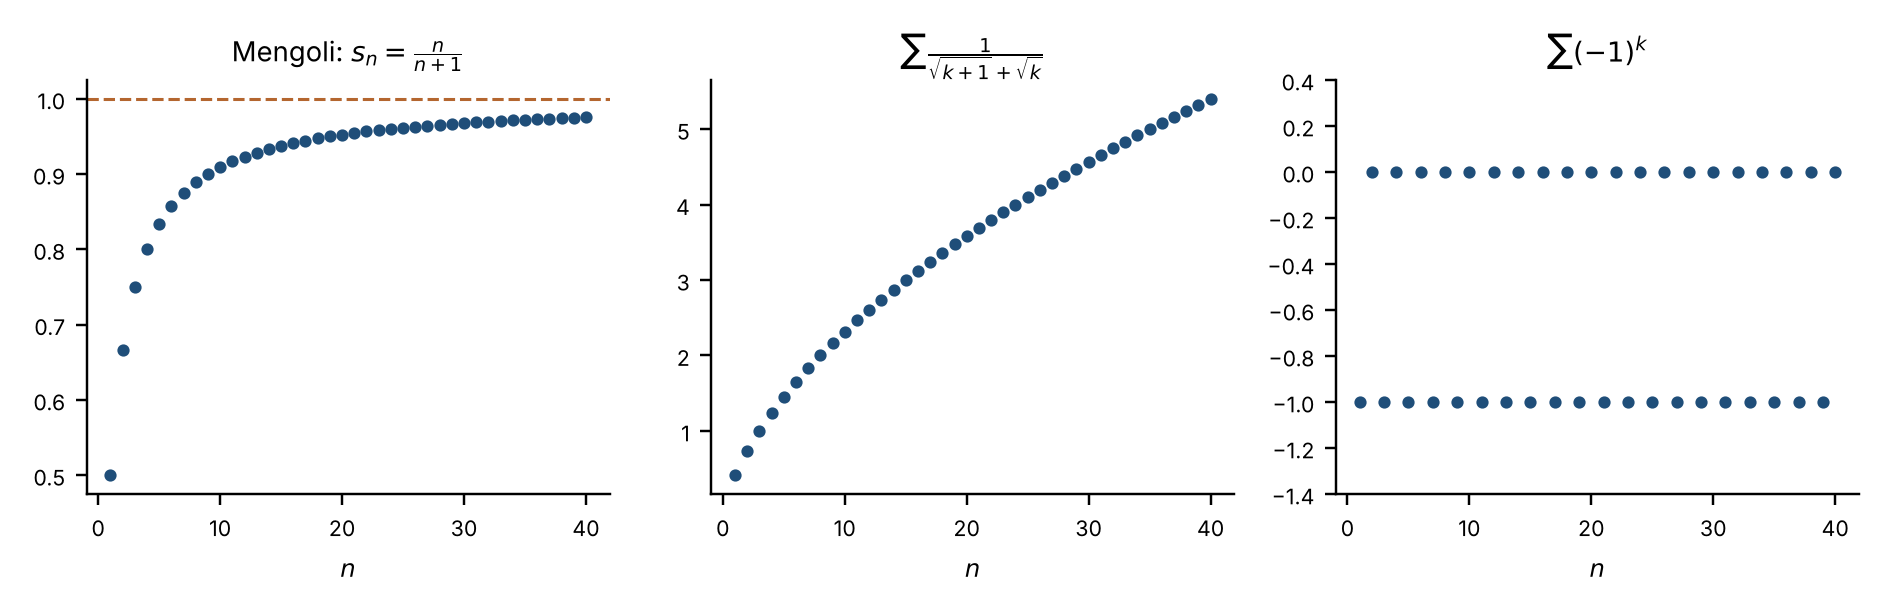
\includegraphics[width=\textwidth]{figure/somme_parziali.png}
\caption{Le somme parziali di tre serie. A sinistra la serie di Mengoli: $s_{n}=\frac n{n+1}$
converge a $1$. Al centro la serie \eqref{eq:serie-radici}: $s_{n}=\sqrt{n+1}-1$ diverge, pur
con termini che tendono a zero. A destra la serie $\sum(-1)^{k}$: le somme parziali
oscillano tra $-1$ e $0$ (\texttt{python/fig\_somme\_parziali.py}).}
\label{fig:somme-parziali}
\end{figure}

\begin{python}[Somme parziali di alcune serie]
import math

def somme_parziali(a, N):
    """Restituisce la lista s_1, ..., s_N delle somme parziali."""
    s, out = 0.0, []
    for k in range(1, N + 1):
        s += a(k)
        out.append(s)
    return out

serie = {
    "Mengoli": lambda k: 1 / (k * (k + 1)),
    "radici":  lambda k: 1 / (math.sqrt(k + 1) + math.sqrt(k)),
    "(-1)^k":  lambda k: (-1)**k,
}
for nome, a in serie.items():
    s = somme_parziali(a, 10000)
    print(f"{nome:8s}: s_10 = {s[9]:9.5f}  s_100 = {s[99]:9.5f}"
          f"  s_10000 = {s[-1]:9.5f}")
\end{python}
\begin{risultato}
Mengoli : s_10 =   0.90909  s_100 =   0.99010  s_10000 =   0.99990
radici  : s_10 =   2.31662  s_100 =   9.04988  s_10000 =  99.00500
(-1)^k  : s_10 =   0.00000  s_100 =   0.00000  s_10000 =   0.00000
\end{risultato}

\needspace{8\baselineskip}
\begin{notastorica}[Da Zenone a Mengoli]
I paradossi di Zenone di Elea (V secolo a.C.), noti attraverso la \emph{Fisica} di
Aristotele, mostrano quanto antica sia la difficoltà di pensare una somma di infiniti
termini. Archimede, nella \emph{Quadratura della parabola}, calcolò di fatto la somma
della serie geometrica $1+\frac14+\frac1{16}+\cdots=\frac43$, evitando però accuratamente
l'infinito con un ragionamento per assurdo (lo abbiamo ripercorso nel
\S\ref{subsec:archimede-parabola}). Non risulta invece che nell'antichità i
paradossi di Zenone siano stati discussi con la serie geometrica: la lettura che ne
daremo nel \S\ref{sec:serie-geometrica} è moderna. Il primo studio sistematico di serie
numeriche si deve al bolognese Pietro Mengoli, allievo di Bonaventura Cavalieri, che nelle
\emph{Novae quadraturae arithmeticae} (1650) sommò la serie che porta il suo nome e altre
serie telescopiche, dimostrò la divergenza della serie armonica e pose il problema di
calcolare $\sum\frac1{k^{2}}$, che sarebbe stato risolto da Eulero quasi un secolo dopo.
\end{notastorica}

%% ----------------------------------------------------------------------------
%%  §11.2  Proprietà delle serie
%% ----------------------------------------------------------------------------
\section{Proprietà delle serie}
\label{sec:proprieta-serie}

Poiché il carattere e la somma di una serie sono definiti mediante il limite delle somme
parziali, le proprietà dei limiti di successioni si traducono in proprietà delle serie.
Cominciamo dalla linearità.

\begin{proposizione}[Linearità]\label{prop:linearita-serie}
\index{serie!linearità}
\begin{enumerate}[label=\textup{(\roman*)}]
  \item Se le serie $\sum a_{k}$ e $\sum b_{k}$ sono regolari e la somma
  $\sum_{k=1}^{\infty}a_{k}+\sum_{k=1}^{\infty}b_{k}$ ha significato in $\overline\R$ (cioè non è della forma
  $+\infty-\infty$), allora la serie $\sum(a_{k}+b_{k})$ è regolare e
  \begin{equation}\label{eq:serie-somma}
    \sum_{k=1}^{\infty}(a_{k}+b_{k})=\sum_{k=1}^{\infty}a_{k}+\sum_{k=1}^{\infty}b_{k} .
  \end{equation}
  \item Se la serie $\sum a_{k}$ è regolare e $c\neq0$ è un numero reale, anche la serie
  $\sum c\,a_{k}$ è regolare e
  \begin{equation}\label{eq:serie-costante}
    \sum_{k=1}^{\infty}c\,a_{k}=c\sum_{k=1}^{\infty}a_{k} ,
  \end{equation}
  con le usuali regole dei segni se la serie diverge. Se $\sum a_{k}$ converge, la
  \eqref{eq:serie-costante} vale anche per $c=0$.
\end{enumerate}
\end{proposizione}

\begin{schema}
\Ipotesi{(i) $\sum a_{k}$, $\sum b_{k}$ regolari, con somme non della forma $+\infty-\infty$; \
(ii) $\sum a_{k}$ regolare, $c\neq0$.}
\Tesi{$\sum(a_{k}+b_{k})=\sum a_{k}+\sum b_{k}$; \ $\sum c\,a_{k}=c\sum a_{k}$.}
\end{schema}

\begin{strategia}
Le somme parziali di $\sum(a_{k}+b_{k})$ e di $\sum c\,a_{k}$ si ottengono da quelle delle serie date
con le operazioni corrispondenti, perché per le somme \emph{finite} le proprietà
associativa, commutativa e distributiva valgono senza restrizioni. Il passaggio al limite
è allora garantito dai teoremi sulle operazioni con i limiti, che escludono proprio le
forme indeterminate $+\infty-\infty$ e $0\cdot\infty$.
\end{strategia}

\begin{dimostrazione}
Le somme parziali di $\sum(a_{k}+b_{k})$ e di $\sum c\,a_{k}$ sono, per le proprietà delle
somme finite, $\sum_{k=1}^{n}(a_{k}+b_{k})=\sum_{k=1}^{n}a_{k}+\sum_{k=1}^{n}b_{k}$ e
$\sum_{k=1}^{n}c\,a_{k}=c\sum_{k=1}^{n}a_{k}$. La tesi segue dai teoremi sulle operazioni con i
limiti, nel caso finito (\cref{teo:operazioni-limiti}) e in quello infinito
(\cref{teo:operazioni-infinite}), esclusi appunto i casi di indeterminazione.
\end{dimostrazione}

Ad esempio, dalla serie di Mengoli si ricava subito
$\sum_{k=1}^{\infty}\frac3{k(k+1)}=3$. Si osservi che la somma di due serie indeterminate può
essere convergente: $\sum(-1)^{k}$ e $\sum(-1)^{k+1}$ sono indeterminate, ma la loro somma è la
serie con tutti i termini nulli.

\subsection{Il resto di una serie}

Le prime somme parziali di una serie possono essere qualsiasi: il carattere dipende
soltanto da ciò che accade «in fondo». Per precisare questa idea, data la serie
$\sum_{k=1}^{\infty}a_{k}$ e fissato $n\in\N$, consideriamo la serie \emph{resto $n$-esimo}
\begin{equation}\label{eq:serie-resto}
  \sum_{k=n+1}^{\infty}a_{k}=a_{n+1}+a_{n+2}+a_{n+3}+\cdots ,
\end{equation}
ottenuta trascurando i primi $n$ termini.

\begin{teorema}[del resto]\label{teo:resto-serie}\index{serie!resto}
Per ogni $n\in\N$ la serie resto $n$-esimo \eqref{eq:serie-resto} ha lo stesso carattere
della serie $\sum_{k=1}^{\infty}a_{k}$. Se la serie converge e $s$ è la sua somma, detta
$R_{n}=\sum_{k=n+1}^{\infty}a_{k}$ la somma del resto, si ha
\begin{equation}\label{eq:resto-serie}
  s=s_{n}+R_{n} \qquad\text{e}\qquad \lim_{n\to+\infty}R_{n}=0 .
\end{equation}
\end{teorema}

\begin{schema}
\Ipotesi{$\sum_{k=1}^{\infty}a_{k}$ serie qualsiasi; \ $n\in\N$ fissato.}
\Tesi{$\sum_{k=n+1}^{\infty}a_{k}$ ha lo stesso carattere di $\sum_{k=1}^{\infty}a_{k}$; \ se
$\sum a_{k}=s\in\R$, allora $R_{n}=s-s_{n}\to0$.}
\end{schema}

\begin{strategia}
Le somme parziali del resto sono differenze di somme parziali della serie data:
$\sum_{k=n+1}^{m}a_{k}=s_{m}-s_{n}$. Con $n$ fissato, $s_{n}$ è una costante, e le due successioni
(nell'indice $m$) hanno lo stesso comportamento. Che il resto tenda a zero è allora la
definizione di convergenza riletta.
\end{strategia}

\begin{dimostrazione}
Fissato $n$, per ogni $m>n$ la somma parziale $(m-n)$-esima del resto è
\[
  \sum_{k=n+1}^{m}a_{k}=\sum_{k=1}^{m}a_{k}-\sum_{k=1}^{n}a_{k}=s_{m}-s_{n} .
\]
Poiché $s_{n}$ non dipende da $m$, la successione $m\mapsto s_{m}-s_{n}$ ha limite (finito o
infinito) se e solo se lo ha $s_{m}$, e i due limiti differiscono per la costante $s_{n}$.
Dunque il resto e la serie hanno lo stesso carattere, e se $s_{m}\to s$ si ha
$R_{n}=\lim_{m\to+\infty}(s_{m}-s_{n})=s-s_{n}$. Infine $R_{n}=s-s_{n}\to s-s=0$ per $n\to+\infty$.
\end{dimostrazione}

Il teorema ha una conseguenza pratica importante: \emph{modificare un numero finito di
termini non cambia il carattere di una serie} (ne cambia, in generale, la somma). Infatti
due serie che differiscono soltanto nei primi $n$ termini hanno lo stesso resto
$n$-esimo. Per questo, nei criteri di convergenza che seguono, le ipotesi potranno essere
richieste soltanto «da un certo indice in poi». Il teorema dice anche che cosa significhi
calcolare la somma di una serie con una somma parziale: l'errore commesso è esattamente
il resto $R_{n}$, e tutto il problema consiste nello \emph{stimarlo}, come abbiamo già fatto
con la formula di Taylor nel \cref{cap:taylor}.

\subsection{Il criterio di Cauchy}

Il criterio di convergenza di Cauchy per le successioni (\cref{teo:criterio-cauchy}),
applicato alle somme parziali, fornisce una condizione necessaria e sufficiente per la
convergenza di una serie che non richiede di conoscerne la somma.

\begin{teorema}[Criterio di Cauchy per le serie]\label{teo:cauchy-serie}
\index{criterio di Cauchy!per le serie}
La serie $\sum_{k=1}^{\infty}a_{k}$ è convergente se e solo se per ogni $\epsilon>0$ esiste
$\nu\in\N$ tale che
\begin{equation}\label{eq:cauchy-serie}
  \Bigl|\sum_{k=n+1}^{n+p}a_{k}\Bigr|=\abs{a_{n+1}+a_{n+2}+\dots+a_{n+p}}<\epsilon
  \qquad\perogni n>\nu,\ \perogni p\in\N .
\end{equation}
\end{teorema}

\begin{schema}
\Ipotesi{$a_{k}$ successione di numeri reali.}
\Tesi{$\sum a_{k}$ convergente $\sse$ $\perogni\epsilon>0\ \esiste\nu$:
$\bigl|\sum_{k=n+1}^{n+p}a_{k}\bigr|<\epsilon$ per ogni $n>\nu$ e ogni $p\in\N$.}
\end{schema}

\begin{strategia}
La serie converge se e solo se la successione $s_{n}$ converge, cioè, per il criterio di
Cauchy, se e solo se $s_{n}$ è di Cauchy. Resta da tradurre la condizione
$\abs{s_{m}-s_{n}}<\epsilon$ in termini degli $a_{k}$: per $m=n+p>n$, la differenza $s_{m}-s_{n}$ è
la somma dei termini da $a_{n+1}$ a $a_{n+p}$.
\end{strategia}

\begin{dimostrazione}
Per il \cref{teo:criterio-cauchy}, la serie converge se e solo se per ogni $\epsilon>0$ esiste
$\nu$ tale che $\abs{s_{m}-s_{n}}<\epsilon$ per ogni $m,n>\nu$. Poiché $\abs{s_{m}-s_{n}}=\abs{s_{n}-s_{m}}$ e
$\abs{s_{n}-s_{n}}=0$, basta considerare le coppie con $m>n$; scritto $m=n+p$ con $p\in\N$,
\[
  s_{m}-s_{n}=\sum_{k=1}^{n+p}a_{k}-\sum_{k=1}^{n}a_{k}=\sum_{k=n+1}^{n+p}a_{k} ,
\]
e la condizione diventa la \eqref{eq:cauchy-serie}.
\end{dimostrazione}

Con $p=1$ la \eqref{eq:cauchy-serie} dà $\abs{a_{n+1}}<\epsilon$ per $n>\nu$: si ritrova la condizione
necessaria del \cref{teo:condizione-necessaria}. Il criterio dice di più: non basta che
i singoli termini siano piccoli, devono essere piccoli anche tutti i «blocchi» di termini
consecutivi, comunque lunghi. Lo useremo per dimostrare il teorema sulla convergenza
assoluta (\S\ref{sec:convergenza-assoluta}) e, nel \S\ref{sec:serie-armonica}, per una terza
dimostrazione della divergenza della serie armonica.

\begin{osservazione}[Parentesi in una serie]\label{oss:parentesi}
Raggruppare con parentesi termini consecutivi di una serie regolare non ne cambia la
somma: le somme parziali della serie raggruppata sono una estratta $s_{n_{1}},s_{n_{2}},\dots$
delle somme parziali della serie data, e un'estratta ha lo stesso limite della
successione (\cref{prop:estratta-limite}). Il viceversa è falso: la serie
$(1-1)+(1-1)+(1-1)+\cdots$ ha tutti i termini nulli e somma $0$, ma togliendo le parentesi si
ottiene la serie indeterminata $1-1+1-1+\cdots$. Le parentesi si possono togliere
liberamente soltanto se si sa già che la serie senza parentesi è regolare.
\end{osservazione}

\begin{osservazione}[Termini nulli]\label{oss:termini-nulli}
Inserire o togliere termini nulli in una serie non ne cambia né il carattere né la
somma. Togliendo gli zeri, infatti, le somme parziali della nuova serie sono un'estratta
di quelle della serie data, e ne hanno lo stesso limite; viceversa, inserendo degli zeri
le somme parziali si ripetono, nello stesso ordine, e le nuove somme parziali hanno lo
stesso limite delle vecchie (se una successione tende a $s$, vi tende anche quella
ottenuta ripetendo un numero finito di volte ciascun termine, come si verifica subito
con la definizione di limite).
\end{osservazione}

%% ----------------------------------------------------------------------------
%%  §11.3  Serie a termini non negativi
%% ----------------------------------------------------------------------------
\section{Serie a termini non negativi}
\label{sec:serie-positive}

Diremo che una serie $\sum a_{k}$ è \emph{a termini non negativi} se $a_{n}\ge0$ per ogni $n$,
e \emph{a termini positivi} se $a_{n}>0$ per ogni $n$. Per queste serie la situazione è
particolarmente semplice, perché la successione delle somme parziali è monotòna: da
$a_{n+1}\ge0$ segue
\begin{equation}\label{eq:somme-crescenti}
  s_{n+1}=s_{n}+a_{n+1}\ge s_{n} \qquad\perogni n\in\N .
\end{equation}

\begin{teorema}[sulle serie a termini non negativi]\label{teo:serie-positive}
\index{serie!a termini non negativi}
Una serie a termini non negativi non può essere indeterminata: è convergente oppure
divergente positivamente. Più precisamente, è convergente se e solo se la successione
delle sue somme parziali è limitata, e in tal caso
\begin{equation}\label{eq:somma-sup}
  \sum_{k=1}^{\infty}a_{k}=\sup_{n\in\N}s_{n} .
\end{equation}
\end{teorema}

\needspace{5\baselineskip}
\begin{schema}
\Ipotesi{$a_{n}\ge0$ per ogni $n$.}
\Tesi{$s_{n}$ ha limite, finito o $+\infty$; \ $\sum a_{k}<+\infty$ $\sse$ $s_{n}$ limitata; \
$\sum a_{k}=\sup s_{n}$.}
\end{schema}

\begin{strategia}
Per la \eqref{eq:somme-crescenti} la successione $s_{n}$ è crescente, e il teorema sulle
successioni monotòne dice tutto: il limite esiste ed è l'estremo superiore, finito se e
solo se la successione è limitata superiormente. Inferiormente $s_{n}$ è limitata da $s_{1}$.
\end{strategia}

\begin{dimostrazione}
Per la \eqref{eq:somme-crescenti} la successione $s_{n}$ è crescente; per il teorema sulle
successioni monotòne (\cref{teo:monotone}) essa ha limite, e $\lim s_{n}=\sup_{n}s_{n}$.
Il limite non può essere $-\infty$, perché $s_{n}\ge s_{1}$ per ogni $n$, e quindi la serie è
convergente o divergente a $+\infty$. Inoltre $\sup_{n}s_{n}<+\infty$ se e solo se $s_{n}$ è
limitata superiormente, cioè (essendo $s_{n}\ge s_{1}$) limitata.
\end{dimostrazione}

In particolare, \emph{la somma di una serie convergente a termini non negativi è
maggiore o uguale a ciascuna delle sue somme parziali}. Per una serie a termini non
negativi si scrive spesso $\sum a_{k}<+\infty$ per dire che la serie converge, e la
condizione necessaria (\cref{teo:condizione-necessaria}) diventa un criterio di
divergenza: se $a_{n}$ non tende a zero, la serie diverge a $+\infty$.

\begin{esempio}\label{es:k-su-k1}
La serie $\sum_{k=1}^{\infty}\frac k{k+1}$ è a termini positivi, quindi convergente o divergente
a $+\infty$. Non è convergente, perché il suo termine generale tende a $1$ e non a $0$.
Dunque $\sum_{k=1}^{\infty}\frac k{k+1}=+\infty$.
\end{esempio}

\begin{esempio}[La serie dei reciproci dei fattoriali]\label{es:serie-fattoriali}
Consideriamo la serie a termini positivi $\sum_{k=0}^{\infty}\frac1{k!}$ (con $0!=1$). Per $k\ge1$
si ha $k!=1\cdot2\cdots k\ge2^{k-1}$, perché ciascuno dei $k-1$ fattori $2,3,\dots,k$ è almeno
$2$. Quindi, per la formula della progressione geometrica (\cref{prop:geometrica}),
\[
  s_{n}=1+\sum_{k=1}^{n}\frac1{k!}\le1+\sum_{k=1}^{n}\frac1{2^{k-1}}=1+\frac{1-2^{-n}}{1-\frac12}<3 :
\]
le somme parziali sono limitate, e la serie converge, con somma compresa tra $s_{1}=2$ e
$3$. La stima del resto \eqref{eq:stima-e} della formula di Taylor dice di più:
$0<e-\sum_{k=0}^{n}\frac1{k!}<\frac3{(n+1)!}\to0$, e quindi
\begin{equation}\label{eq:e-serie}
  \sum_{k=0}^{\infty}\frac1{k!}=1+1+\frac12+\frac1{3!}+\frac1{4!}+\dots=e .
\end{equation}
Il teorema sulle serie a termini non negativi ha garantito l'\emph{esistenza} della
somma con un ragionamento elementare; la formula di Taylor ne ha fornito il
\emph{valore}. (Lo stesso valore si ottiene anche senza Taylor, direttamente dalla
definizione di $e$ come limite di $\bigl(1+\frac1n\bigr)^{n}$: si veda
l'\cref{oss:e-due-vie}.) È il metodo efficiente per il calcolo di $e$ annunciato nel
\cref{cap:successioni}: undici termini danno sette cifre decimali esatte, mentre la
successione $\bigl(1+\frac1n\bigr)^{n}$ ne dà appena cinque con $n=10^{6}$.
\end{esempio}

%% ----------------------------------------------------------------------------
%%  §11.4  La serie geometrica
%% ----------------------------------------------------------------------------
\section{La serie geometrica}
\label{sec:serie-geometrica}

Per ogni numero reale $x$ consideriamo la \emph{serie geometrica} di \emph{ragione} $x$
\begin{equation}\label{eq:serie-geometrica-def}
  \sum_{k=0}^{\infty}x^{k}=1+x+x^{2}+\dots+x^{n}+\cdots .
\end{equation}
È la serie più importante di tutta la teoria: è una delle pochissime di cui si conosce
esplicitamente la somma parziale, e servirà da termine di paragone per molte altre.

\begin{teorema}[Serie geometrica]\label{teo:serie-geometrica}\index{serie!geometrica}
La serie geometrica di ragione $x$ è convergente se $\abs x<1$, divergente
positivamente se $x\ge1$, indeterminata se $x\le-1$. Inoltre
\begin{equation}\label{eq:serie-geometrica}
  \sum_{k=0}^{\infty}x^{k}=\frac1{1-x} \qquad\text{se } -1<x<1 .
\end{equation}
\end{teorema}

\begin{schema}
\Ipotesi{$x\in\R$.}
\Tesi{$\sum x^{k}=\frac1{1-x}$ se $\abs x<1$; \ $\sum x^{k}=+\infty$ se $x\ge1$; \ $\sum x^{k}$
indeterminata se $x\le-1$.}
\end{schema}

\begin{strategia}
Per $x\neq1$ la somma parziale è nota esplicitamente, $s_{n}=\frac{1-x^{n+1}}{1-x}$, e il suo
comportamento dipende soltanto da quello di $x^{n+1}$, che conosciamo dal capitolo sulle
successioni. Il caso $x=1$ si tratta a parte.
\end{strategia}

\begin{dimostrazione}
Se $x=1$, $s_{n}=n+1\to+\infty$. Se $x\neq1$, per la \cref{prop:geometrica}
\begin{equation}\label{eq:somma-parziale-geometrica}
  s_{n}=\sum_{k=0}^{n}x^{k}=\frac{1-x^{n+1}}{1-x} .
\end{equation}
Per il \cref{teo:lim-geometrica}, $x^{n+1}\to0$ se $-1<x<1$, $x^{n+1}\to+\infty$ se $x>1$, e
$x^{n+1}$ non ha limite se $x\le-1$. Nel primo caso $s_{n}\to\frac1{1-x}$. Nel secondo, poiché
$1-x<0$, $s_{n}=\frac{x^{n+1}-1}{x-1}\to+\infty$. Nel terzo, se $s_{n}$ avesse limite $\ell$, anche
$x^{n+1}=1-(1-x)s_{n}$ avrebbe limite $1-(1-x)\ell$ (finito o infinito), il che è falso.
\end{dimostrazione}

Moltiplicando per una costante (\cref{prop:linearita-serie}) e trascurando i primi
termini, si ottiene la forma in cui la serie geometrica si usa più spesso: per $\abs x<1$,
$a\in\R$ e $m\ge0$ intero,
\begin{equation}\label{eq:geometrica-generale}
  \sum_{k=m}^{\infty}a\,x^{k}=a\,x^{m}+a\,x^{m+1}+\dots=\frac{a\,x^{m}}{1-x} ,
\end{equation}
cioè «il primo termine diviso per uno meno la ragione». Ad esempio
$\frac12+\frac14+\frac18+\cdots=\frac{1/2}{1-1/2}=1$, come mostra la \cref{fig:quadrato-geometrico}.

\begin{figure}[htb]
\centering
\begin{tikzpicture}[scale=3.2]
  \fill[blu!35] (0,0) rectangle (0.5,1);
  \fill[blu!25] (0.5,0) rectangle (1,0.5);
  \fill[blu!17] (0.5,0.5) rectangle (0.75,1);
  \fill[blu!11] (0.75,0.5) rectangle (1,0.75);
  \fill[blu!7]  (0.75,0.75) rectangle (0.875,1);
  \fill[blu!4]  (0.875,0.75) rectangle (1,0.875);
  \draw[blu] (0,0) rectangle (1,1);
  \draw[blu] (0.5,0) -- (0.5,1) (0.5,0.5) -- (1,0.5) (0.75,0.5) -- (0.75,1)
    (0.75,0.75) -- (1,0.75) (0.875,0.75) -- (0.875,1) (0.875,0.875) -- (1,0.875);
  \node[font=\small] at (0.25,0.5) {$\frac12$};
  \node[font=\small] at (0.75,0.25) {$\frac14$};
  \node[font=\footnotesize] at (0.625,0.75) {$\frac18$};
  \node[font=\scriptsize] at (0.875,0.625) {$\frac1{16}$};
  \node[font=\tiny] at (0.8125,0.875) {$\frac1{32}$};
\end{tikzpicture}
\caption{La serie geometrica $\frac12+\frac14+\frac18+\cdots=1$: ogni rettangolo è metà della
parte del quadrato unitario non ancora coperta, e i rettangoli riempiono l'intero
quadrato. Le somme parziali sono $1-\frac1{2^{n}}$.}
\label{fig:quadrato-geometrico}
\end{figure}

\subsection{I numeri decimali periodici}

Con la serie geometrica possiamo giustificare la regola, nota dalla scuola media, con
cui un numero decimale periodico si trasforma nella sua \emph{frazione generatrice}. Un
allineamento decimale infinito $0{,}c_{1}c_{2}c_{3}\ldots$, con cifre $c_{k}\in\{0,1,\dots,9\}$, è per
definizione la somma della serie a termini non negativi $\sum_{k=1}^{\infty}c_{k}10^{-k}$, che
converge perché le sue somme parziali sono limitate da $\sum_{k=1}^{\infty}9\cdot10^{-k}=1$.

\begin{proposizione}[Frazione generatrice]\label{prop:periodici}
Sia $0{,}\overline{c_{1}c_{2}\ldots c_{p}}$ un numero decimale periodico semplice con periodo di $p$
cifre, e sia $C=c_{1}c_{2}\ldots c_{p}$ l'intero che ha quelle cifre. Allora
\begin{equation}\label{eq:periodici}
  0{,}\overline{c_{1}c_{2}\ldots c_{p}}=\frac C{10^{p}-1}=\frac C{99\ldots9} ,
\end{equation}
dove il denominatore $99\ldots9$ è formato da $p$ cifre uguali a $9$. In particolare, ogni
numero decimale periodico è razionale.
\end{proposizione}

\begin{schema}
\Ipotesi{$0{,}\overline{c_{1}\ldots c_{p}}=\sum_{k=1}^{\infty}c_{k}10^{-k}$ con $c_{k+p}=c_{k}$; \ $C=c_{1}c_{2}\ldots c_{p}$.}
\Tesi{$0{,}\overline{c_{1}\ldots c_{p}}=\frac C{10^{p}-1}$.}
\end{schema}

\begin{strategia}
Le cifre si ripetono a blocchi di $p$: ogni blocco vale $C$ volte una potenza di
$10^{-p}$, e raggruppando i termini a blocchi la serie delle cifre diventa una serie
geometrica di ragione $10^{-p}$, di cui conosciamo la somma.
\end{strategia}

\begin{dimostrazione}
Il numero è la somma della serie in cui il blocco di cifre si ripete: il primo blocco
vale $C\cdot10^{-p}$, il secondo $C\cdot10^{-2p}$, e così via. Raggruppando le cifre a blocchi
di $p$ (\cref{oss:parentesi}) e usando la \eqref{eq:geometrica-generale} con $x=10^{-p}$,
\[
  0{,}\overline{c_{1}\ldots c_{p}}=\sum_{j=1}^{\infty}C\,10^{-jp}=\frac{C\,10^{-p}}{1-10^{-p}}=\frac C{10^{p}-1} .
\]
Un numero periodico misto si riconduce a questo caso moltiplicando per una potenza di
$10$ e sottraendo l'antiperiodo, che è un numero razionale.
\end{dimostrazione}

Ad esempio $0{,}\overline{13}=\frac{13}{99}$, e $0{,}\overline{9}=\frac99=1$: l'allineamento $0{,}999\ldots$
\emph{non} è «un po' meno» di $1$, ma è esattamente $1$, perché la sua somma è il
\emph{limite} delle somme parziali $1-10^{-n}$. Molte perplessità sull'uguaglianza
$0{,}\overline9=1$ nascono proprio dal confondere una serie con le sue somme parziali.

\subsection{Il paradosso di Achille}

\begin{idea}[Achille e la tartaruga, in volo]
Un velivolo $A$ insegue alla velocità $v_{A}$ un velivolo $B$ che lo precede di una
distanza $d$ e vola sulla stessa rotta alla velocità $v_{B}<v_{A}$. Ragioniamo come
Zenone (\cref{fig:zenone}). Nel tempo $t_{0}=\frac d{v_{A}}$ che $A$ impiega a raggiungere la
posizione iniziale di $B$, questo avanza di $d\,\frac{v_{B}}{v_{A}}$; nel tempo $t_{1}=t_{0}\frac{v_{B}}{v_{A}}$ che
$A$ impiega a colmare questo nuovo distacco, $B$ avanza di $d\bigl(\frac{v_{B}}{v_{A}}\bigr)^{2}$; e così
via. I tempi $t_{k}=t_{0}q^{k}$, con $q=\frac{v_{B}}{v_{A}}<1$, sono infiniti, ma la loro somma è la
serie geometrica
\[
  T=\sum_{k=0}^{\infty}\frac d{v_{A}}\,q^{k}=\frac d{v_{A}}\cdot\frac1{1-\frac{v_{B}}{v_{A}}}=\frac d{v_{A}-v_{B}} ,
\]
che è finita, ed è proprio il tempo che si ottiene ragionando con la velocità relativa
$v_{A}-v_{B}$. Ad esempio, con $d=20$~km, $v_{A}=900$~km/h e $v_{B}=750$~km/h, il
raggiungimento avviene dopo $T=\frac{20}{150}$~h, cioè $8$~minuti. Dal punto di vista matematico, il
paradosso nasce dal supporre che infiniti intervalli di tempo debbano avere una durata
complessiva infinita. (Aristotele, che riferisce l'argomento, rispondeva distinguendo
l'infinito «in atto» da quello «in potenza»: un dibattito filosofico che la definizione
di somma di una serie non esaurisce, ma rende innocuo per il calcolo.)
\end{idea}

\begin{figure}[htb]
\centering
\begin{tikzpicture}[x=0.95cm]
  \draw[grigio, -{Stealth[length=2mm]}] (-0.3,0) -- (10.6,0) node[above, font=\scriptsize] {rotta};
  \foreach \x/\lab in {0/{$A_{0}$}, 4/{$A_{1}=B_{0}$}, 6.4/{$A_{2}=B_{1}$}, 7.84/{$B_{2}$}}
    \fill (\x,0) circle (1.4pt) node[below=2pt, font=\scriptsize] {\lab};
  \fill (8.704,0) circle (1pt);
  \fill (9.222,0) circle (1pt);
  \fill (9.533,0) circle (0.8pt);
  \draw[rame, thick] (10,-0.12) -- (10,0.12);
  \node[rame, font=\scriptsize, below=2pt] at (10,0) {incontro};
  \draw[blu, -{Stealth[length=1.6mm]}] (0,0.35) -- node[above, font=\scriptsize] {$t_{0}$} (4,0.35);
  \draw[blu, -{Stealth[length=1.6mm]}] (4,0.35) -- node[above, font=\scriptsize] {$t_{1}=qt_{0}$} (6.4,0.35);
  \draw[blu, -{Stealth[length=1.6mm]}] (6.4,0.35) -- node[above, font=\scriptsize] {$t_{2}$} (7.84,0.35);
  \draw[blu, -{Stealth[length=1.6mm]}] (7.84,0.35) -- (8.704,0.35);
\end{tikzpicture}
\caption{Il ragionamento di Zenone per l'inseguimento ($q=\frac{v_{B}}{v_{A}}=0{,}6$ nel disegno):
$A$ raggiunge successivamente le posizioni $B_{0},B_{1},B_{2},\dots$ occupate da $B$ un passo
prima. I tratti, e i tempi, formano una progressione geometrica di ragione $q$, e la loro
somma è finita: l'incontro avviene a distanza $\frac d{1-q}$ dal punto di partenza di $A$.}
\label{fig:zenone}
\end{figure}

\begin{python}[Serie geometrica e frazioni generatrici]
from fractions import Fraction as F

def periodico(antiperiodo, periodo):
    """Frazione di 0,antiperiodo(periodo), es. ('1', '6') -> 1/6."""
    m, p = len(antiperiodo), len(periodo)
    A = int(antiperiodo) if antiperiodo else 0
    C = int(periodo)
    # 0,a(c) = (A + C/(10^p - 1)) / 10^m
    return (A + F(C, 10**p - 1)) / 10**m

for a, c in (("", "13"), ("", "9"), ("1", "6"), ("", "142857")):
    print(f"0,{a}({c}) = {periodico(a, c)}")

x = 0.6                                    # somme parziali, q = 0,6
s = [sum(x**k for k in range(n + 1)) for n in (5, 10, 20, 40)]
print("s_n:", [round(v, 8) for v in s], " 1/(1-x) =", 1 / (1 - x))
\end{python}
\begin{risultato}
0,(13) = 13/99
0,(9) = 1
0,1(6) = 1/6
0,(142857) = 1/7
s_n: [2.38336, 2.49093007, 2.49994516, 2.5]  1/(1-x) = 2.5
\end{risultato}

\begin{notastorica}[Eulero e le «somme» delle serie divergenti]
La formula \eqref{eq:serie-geometrica} vale soltanto per $-1<x<1$, ma per tutto il
Settecento fu usata spesso senza questa restrizione. Con $x=-1$ se ne ricava
$1-1+1-1+\cdots=\frac12$: il camaldolese Guido Grandi, professore a Pisa, vi vide nel 1703
un'immagine della creazione dal nulla, e Leibniz, in una lettera a Christian Wolff
pubblicata nel 1713, difese il valore $\frac12$ osservando che le somme parziali valgono $1$
e $0$ «con uguale probabilità». Con $x=2$ si ottiene addirittura $-1=1+2+4+8+\cdots$.
Eulero discusse proprio questa uguaglianza nella memoria \emph{De seriebus divergentibus}
(1760), e propose di chiamare somma di una serie l'espressione finita dal cui sviluppo
essa nasce, qui $\frac1{1-x}$: nelle sue mani la regola condusse a scoperte profonde, in mani
meno esperte a contraddizioni. Cauchy, nel \emph{Cours d'analyse} (1821), tagliò il nodo
con la definizione che abbiamo adottato: una serie divergente non ha somma, e le
operazioni sulle serie sono lecite soltanto per quelle convergenti. Nel 1826 il giovane
Niels Henrik Abel scriveva a un amico che le serie divergenti sono «qualcosa di funesto»,
su cui è una vergogna fondare una dimostrazione. Più tardi si capì come recuperare in
modo coerente almeno una parte di quei valori: Ernesto Cesàro (1890) propose di
sostituire alle somme parziali le loro medie aritmetiche, che per la serie di Grandi
tendono proprio a $\frac12$. Nacque così la teoria della \emph{sommabilità}, che non
contraddice la definizione di Cauchy, ma la estende.
\end{notastorica}

%% ----------------------------------------------------------------------------
%%  §11.5  La serie armonica
%% ----------------------------------------------------------------------------
\section{La serie armonica}
\label{sec:serie-armonica}

La serie
\begin{equation}\label{eq:serie-armonica}
  \sum_{k=1}^{\infty}\frac1k=1+\frac12+\frac13+\dots+\frac1n+\cdots
\end{equation}
si chiama \emph{serie armonica}\index{serie!armonica}. Il suo termine generale tende a zero,
e le somme parziali crescono molto lentamente: ci vogliono più di dodicimila termini
perché superino $10$. Eppure la serie diverge. Poiché il risultato è importante e un po'
sorprendente, ne diamo tre dimostrazioni, ciascuna delle quali insegna qualcosa.

\begin{teorema}[Divergenza della serie armonica]\label{teo:armonica}
La serie armonica è divergente: $\sum_{k=1}^{\infty}\frac1k=+\infty$. Più precisamente, le sue
somme parziali $H_{n}=\sum_{k=1}^{n}\frac1k$ verificano
\begin{equation}\label{eq:armonica-log}
  H_{n}\ge\log(n+1) \qquad\perogni n\in\N .
\end{equation}
\end{teorema}

\begin{schema}
\Ipotesi{$H_{n}=\sum_{k=1}^{n}\frac1k$.}
\Tesi{$H_{n}\ge\log(n+1)$ per ogni $n$; \ quindi $H_{n}\to+\infty$.}
\end{schema}

\begin{strategia}
Confrontiamo la somma con un'area. Il termine $\frac1k$ è l'area di un rettangolo di base
$[k,k+1]$ e altezza $\frac1k$, che contiene la regione sotto il grafico di $\frac1x$ nello stesso
intervallo, perché $\frac1x\le\frac1k$ per $x\ge k$ (\cref{fig:armonica-integrale}, a sinistra).
Sommando, $H_{n}$ supera l'integrale di $\frac1x$ tra $1$ e $n+1$, cioè $\log(n+1)$, che diverge.
\end{strategia}

\begin{dimostrazione}[Prima dimostrazione (con l'integrale)]
Per ogni $k\in\N$ e ogni $x\in[k,k+1]$ si ha $\frac1x\le\frac1k$. Per il confronto tra integrali
(\cref{teo:confronto-integrali}),
\begin{equation}\label{eq:armonica-rettangolo}
  \int_{k}^{k+1}\frac{dx}x\le\int_{k}^{k+1}\frac{dx}k=\frac1k .
\end{equation}
Sommando per $k$ da $1$ a $n$ e usando l'additività dell'integrale (\cref{teo:additivita})
e la formula fondamentale del calcolo integrale,
\[
  H_{n}=\sum_{k=1}^{n}\frac1k\ge\sum_{k=1}^{n}\int_{k}^{k+1}\frac{dx}x=\int_{1}^{n+1}\frac{dx}x=\log(n+1) .
\]
Poiché $\log(n+1)\to+\infty$, per il teorema del confronto (\cref{teo:confronto-infinito})
anche $H_{n}\to+\infty$.
\end{dimostrazione}

La seconda dimostrazione ottiene la stessa disuguaglianza senza il calcolo integrale,
usando le proprietà del numero $e$.

\begin{dimostrazione}[Seconda dimostrazione (con il numero $e$)]
Per il \cref{teo:numero-e} si ha $\bigl(1+\frac1k\bigr)^{k}<e$ per ogni $k\in\N$. Poiché il
logaritmo è crescente,
\[
  k\log\Bigl(1+\frac1k\Bigr)=\log\Bigl(1+\frac1k\Bigr)^{k}<\log e=1 ,
\]
cioè
\[
  \frac1k>\log\frac{k+1}k=\log(k+1)-\log k .
\]
Sommando per $k=1,\dots,n$, il secondo membro è una somma telescopica
(\cref{prop:serie-telescopica}):
$H_{n}>\log(n+1)-\log1=\log(n+1)$.
\end{dimostrazione}

La terza dimostrazione, la più antica, raggruppa i termini a blocchi e usa il criterio di
Cauchy.

\begin{dimostrazione}[Terza dimostrazione (con il criterio di Cauchy)]
Per ogni $n\in\N$, il blocco dei $n$ termini da $\frac1{n+1}$ a $\frac1{2n}$ verifica
\[
  \sum_{k=n+1}^{2n}\frac1k=\frac1{n+1}+\frac1{n+2}+\dots+\frac1{2n}\ge n\cdot\frac1{2n}=\frac12 ,
\]
perché ciascuno dei suoi $n$ termini è almeno $\frac1{2n}$. Dunque la condizione
\eqref{eq:cauchy-serie} è violata con $\epsilon=\frac12$ e $p=n$, per ogni $n$: la serie non
converge (\cref{teo:cauchy-serie}). Essendo a termini positivi, diverge a $+\infty$
(\cref{teo:serie-positive}).
\end{dimostrazione}

\begin{figure}[htb]
\centering
\begin{tikzpicture}
\begin{axis}[width=0.53\textwidth, height=4.6cm, xmin=0, xmax=8.6, ymin=0, ymax=1.15,
  axis lines=left, xtick={1,2,...,8}, ytick={0,0.5,1}, axis on top,
  title={\scriptsize $H_{n}\ge\int_{1}^{n+1}\frac{dx}x$}, tick label style={font=\scriptsize}]
  \addplot[fill=blu!20, draw=blu, ybar interval]
    coordinates {(1,1) (2,0.5) (3,0.3333) (4,0.25) (5,0.2) (6,0.1667) (7,0.1429) (8,0)};
  \addplot[curva, domain=0.87:8.6, samples=80] {1/x};
\end{axis}
\end{tikzpicture}\hfill
\begin{tikzpicture}
\begin{axis}[width=0.53\textwidth, height=4.6cm, xmin=0, xmax=8.6, ymin=0, ymax=1.15,
  axis lines=left, xtick={1,2,...,8}, ytick={0,0.5,1}, axis on top,
  title={\scriptsize $H_{n+1}-1\le\int_{1}^{n+1}\frac{dx}x$}, tick label style={font=\scriptsize}]
  \addplot[fill=rame!30, draw=rame, ybar interval]
    coordinates {(1,0.5) (2,0.3333) (3,0.25) (4,0.2) (5,0.1667) (6,0.1429) (7,0.125) (8,0)};
  \addplot[curva, domain=0.87:8.6, samples=80] {1/x};
\end{axis}
\end{tikzpicture}
\caption{Il confronto tra la serie armonica e l'integrale di $\frac1x$. A sinistra i
rettangoli di altezza $\frac1k$ sulle basi $[k,k+1]$ contengono la regione sotto il grafico:
$H_{n}\ge\log(n+1)$. A destra i rettangoli di altezza $\frac1{k+1}$ sono contenuti in essa:
$H_{n+1}-1\le\log(n+1)$. Le somme parziali sono quindi «intrappolate» tra due logaritmi.}
\label{fig:armonica-integrale}
\end{figure}

\subsection{Il criterio dell'integrale e la serie armonica generalizzata}

Il ragionamento della prima dimostrazione funziona per ogni funzione positiva e
decrescente, e collega il carattere di una serie a quello di un integrale improprio
(\S\ref{sec:impropri}).

\begin{teorema}[Criterio dell'integrale]\label{teo:criterio-integrale}
\index{criterio dell'integrale}
Sia $f$ continua, non negativa e decrescente in $[1,+\infty)$, e sia $a_{k}=f(k)$. Allora
per ogni $n\in\N$
\begin{equation}\label{eq:criterio-integrale}
  \int_{1}^{n+1}f(x)\,dx\le\sum_{k=1}^{n}a_{k}\le a_{1}+\int_{1}^{n}f(x)\,dx ,
\end{equation}
e la serie $\sum_{k=1}^{\infty}a_{k}$ converge se e solo se converge l'integrale improprio
$\int_{1}^{+\infty}f(x)\,dx$. In tal caso il resto $R_{n}=\sum_{k=n+1}^{\infty}a_{k}$ verifica
\begin{equation}\label{eq:resto-integrale-serie}
  \int_{n+1}^{+\infty}f(x)\,dx\le R_{n}\le\int_{n}^{+\infty}f(x)\,dx .
\end{equation}
\end{teorema}

\begin{schema}
\Ipotesi{$f$ continua, $f\ge0$, decrescente in $[1,+\infty)$; \ $a_{k}=f(k)$.}
\Tesi{la \eqref{eq:criterio-integrale}; \ $\sum a_{k}<+\infty$ $\sse$
$\int_{1}^{+\infty}f<+\infty$; \ la stima \eqref{eq:resto-integrale-serie} del resto.}
\end{schema}

\begin{strategia}
Come nella \cref{fig:armonica-integrale}: nell'intervallo $[k,k+1]$ la funzione
decrescente sta tra $f(k+1)$ e $f(k)$, e integrando si ottiene
$a_{k+1}\le\int_{k}^{k+1}f\le a_{k}$. Sommando si ottengono le due stime. Le somme parziali e la
funzione integrale $b\mapsto\int_{1}^{b}f$ sono entrambe crescenti, e le stime dicono che una è
limitata se e solo se lo è l'altra.
\end{strategia}

\begin{dimostrazione}
Per $x\in[k,k+1]$ la monotonia dà $f(k+1)\le f(x)\le f(k)$, e per il confronto tra
integrali
\begin{equation}\label{eq:integrale-intrappolato}
  a_{k+1}\le\int_{k}^{k+1}f(x)\,dx\le a_{k} \qquad\perogni k\in\N .
\end{equation}
Sommando la disuguaglianza di destra per $k=1,\dots,n$ si ottiene
$\int_{1}^{n+1}f\le\sum_{k=1}^{n}a_{k}$; sommando quella di sinistra per $k=1,\dots,n-1$ si ottiene
$\sum_{k=2}^{n}a_{k}\le\int_{1}^{n}f$, cioè la seconda delle \eqref{eq:criterio-integrale}.

Poiché $f\ge0$, la funzione $F(b)=\int_{1}^{b}f$ è crescente, e per il \cref{lem:monotona-infinito}
ha limite per $b\to+\infty$, finito se e solo se $F$ è limitata; inoltre, essendo crescente,
$F$ è limitata se e solo se lo è la successione $F(n)$. Le \eqref{eq:criterio-integrale}
mostrano che $s_{n}$ è limitata se e solo se $F(n)$ lo è, e per il \cref{teo:serie-positive}
la serie converge se e solo se converge l'integrale.

Infine, sommando le \eqref{eq:integrale-intrappolato} per $k$ da $n+1$ a $m$ si ha
$\int_{n+1}^{m+1}f\le\sum_{k=n+1}^{m}a_{k}$ e, per $k$ da $n$ a $m-1$, $\sum_{k=n+1}^{m}a_{k}\le\int_{n}^{m}f$;
per $m\to+\infty$ si ottiene la \eqref{eq:resto-integrale-serie}.
\end{dimostrazione}

\begin{teorema}[Serie armonica generalizzata]\label{teo:armonica-generalizzata}
\index{serie!armonica generalizzata}
La serie
\begin{equation}\label{eq:armonica-generalizzata}
  \sum_{k=1}^{\infty}\frac1{k^{p}}=1+\frac1{2^{p}}+\frac1{3^{p}}+\dots+\frac1{n^{p}}+\cdots
\end{equation}
è convergente se $p>1$ ed è divergente se $p\le1$.
\end{teorema}

\begin{schema}
\Ipotesi{$p\in\R$.}
\Tesi{$\sum\frac1{k^{p}}<+\infty$ $\sse$ $p>1$.}
\end{schema}

\begin{strategia}
Per $p>0$ la funzione $\frac1{x^{p}}$ è positiva e decrescente, e il criterio dell'integrale
riduce il problema all'integrale improprio $\int_{1}^{+\infty}\frac{dx}{x^{p}}$, già calcolato nel
\cref{cap:integrali-indefiniti}. Per $p\le0$ il termine generale non tende a zero.
\end{strategia}

\begin{dimostrazione}
Se $p\le0$, $\frac1{k^{p}}=k^{-p}\ge1$ non tende a zero, e la serie (a termini positivi) diverge
per il \cref{teo:condizione-necessaria}. Se $p>0$, la funzione $f(x)=x^{-p}$ è continua,
positiva e decrescente in $[1,+\infty)$; per il \cref{teo:criterio-integrale} e la
\eqref{eq:impropri-p-infinito}, la serie converge se e solo se $p>1$.
\end{dimostrazione}

Per $p>1$ la \eqref{eq:criterio-integrale} dà anche
$\frac{(n+1)^{1-p}-1}{1-p}\le s_{n}\le1+\frac{1-n^{1-p}}{p-1}$, e passando al limite
$\frac1{p-1}\le\sum_{k=1}^{\infty}\frac1{k^{p}}\le\frac p{p-1}$. Ad esempio $1\le\sum\frac1{k^{2}}\le2$; il valore esatto
è $\frac{\pi^{2}}6\approx1{,}6449$, come scoprì Eulero nel 1734. La stima del resto
\eqref{eq:resto-integrale-serie} con $f(x)=\frac1{x^{2}}$ dice che
$\frac1{n+1}\le\frac{\pi^{2}}6-\sum_{k=1}^{n}\frac1{k^{2}}\le\frac1n$: con cento termini si ottiene una sola cifra
decimale esatta (l'errore è circa $10^{-2}$).

\subsection{La costante di Eulero--Mascheroni}

Le somme parziali della serie armonica divergono, ma in modo molto regolare: sono vicine
a $\log n$, e la differenza ha un limite.

\begin{proposizione}[Costante di Eulero--Mascheroni]\label{prop:eulero-mascheroni}
\index{costante di Eulero--Mascheroni}
La successione $d_{n}=H_{n}-\log n$ è decrescente e verifica $0\le d_{n}\le1$. Il suo limite
\begin{equation}\label{eq:eulero-mascheroni}
  \gamma=\lim_{n\to+\infty}\Bigl(1+\frac12+\dots+\frac1n-\log n\Bigr)=0{,}5772156649\ldots
\end{equation}
si chiama \emph{costante di Eulero--Mascheroni}. In particolare $H_{n}=\log n+\gamma+o(1)$.
\end{proposizione}

\begin{schema}
\Ipotesi{$d_{n}=H_{n}-\log n$.}
\Tesi{$d_{n+1}\le d_{n}$; \ $0\le d_{n}\le1$; \ quindi $d_{n}\to\gamma\in[0,1]$.}
\end{schema}

\begin{strategia}
Basta mostrare che $d_{n}$ è monotòna e limitata. La differenza $d_{n}-d_{n+1}$ è l'area compresa,
nell'intervallo $[n,n+1]$, tra il grafico di $\frac1x$ e il rettangolo di altezza $\frac1{n+1}$:
è positiva. La limitazione dal basso viene dalla stima \eqref{eq:armonica-log}, che dice
che $H_{n}$ supera $\log(n+1)$, e quindi anche $\log n$.
\end{strategia}

\begin{dimostrazione}
Si ha $d_{n}-d_{n+1}=\log(n+1)-\log n-\frac1{n+1}=\int_{n}^{n+1}\bigl(\frac1x-\frac1{n+1}\bigr)dx\ge0$,
perché l'integrando è non negativo in $[n,n+1]$: la successione è decrescente, e quindi
$d_{n}\le d_{1}=1$. Inoltre, per la \eqref{eq:armonica-log},
$d_{n}\ge\log(n+1)-\log n>0$. Per il teorema sulle successioni monotòne $d_{n}$ converge a un
limite $\gamma\in[0,1]$.
\end{dimostrazione}

La relazione $H_{n}\approx\log n+\gamma$ spiega la lentezza della divergenza: per avere
$H_{n}>10$ occorre $n\approx e^{10-\gamma}\approx12\,367$, e per $H_{n}>100$ un numero di termini
dell'ordine di $10^{43}$. Non si sa ancora se $\gamma$ sia un numero razionale.

\begin{python}[Serie armonica, costante di Eulero e problema di Basilea]
import math

H, n = 0.0, 0
while H <= 10:                        # primo n con H_n > 10
    n += 1
    H += 1 / n
print(f"H_n > 10 per la prima volta con n = {n}")

H, N = 0.0, 1
for k in range(1, 10**6 + 1):
    H += 1 / k
    if k == N:
        print(f"n = {k:>7}:  H_n - log n = {H - math.log(k):.8f}")
        N *= 10

s = sum(1 / k**2 for k in range(1, 101))
print(f"pi^2/6 - s_100 = {math.pi**2 / 6 - s:.6f}"
      f"   (stima: tra {1/101:.6f} e {1/100:.6f})")
\end{python}
\begin{risultato}
H_n > 10 per la prima volta con n = 12367
n =       1:  H_n - log n = 1.00000000
n =      10:  H_n - log n = 0.62638316
n =     100:  H_n - log n = 0.58220733
n =    1000:  H_n - log n = 0.57771558
n =   10000:  H_n - log n = 0.57726566
n =  100000:  H_n - log n = 0.57722066
n = 1000000:  H_n - log n = 0.57721616
pi^2/6 - s_100 = 0.009950   (stima: tra 0.009901 e 0.010000)
\end{risultato}

\subsection{Approfondimento: il criterio di condensazione di Cauchy}
\label{subsec:condensazione}

La terza dimostrazione della divergenza della serie armonica raggruppava i termini in
blocchi sempre più lunghi. Se i blocchi hanno lunghezza $1,2,4,8,\dots$, l'idea funziona
per ogni successione non negativa e decrescente, e conduce a un criterio, dovuto a
Cauchy (\emph{Cours d'analyse}, 1821), che non richiede il calcolo integrale: la serie
data ha lo stesso carattere di una serie formata soltanto dai termini di indice $2^{k}$,
ciascuno moltiplicato per $2^{k}$, cioè per il numero dei termini del blocco che
rappresenta.

\begin{teorema}[Criterio di condensazione]\label{teo:condensazione}
\index{criterio di condensazione}
Sia $a_{n}$ una successione non negativa e decrescente. Allora le serie
\begin{equation}\label{eq:condensazione}
  \sum_{n=1}^{\infty}a_{n} \qquad\text{e}\qquad
  \sum_{k=0}^{\infty}2^{k}a_{2^{k}}=a_{1}+2a_{2}+4a_{4}+8a_{8}+\cdots
\end{equation}
hanno lo stesso carattere. Più precisamente, dette $s_{n}=\sum_{j=1}^{n}a_{j}$ e
$t_{m}=\sum_{k=0}^{m}2^{k}a_{2^{k}}$ le somme parziali delle due serie, per ogni intero $m\ge0$
\begin{equation}\label{eq:condensazione-stime}
  \tfrac12\,t_{m}\le s_{2^{m}} \qquad\text{e}\qquad s_{2^{m+1}-1}\le t_{m} .
\end{equation}
\end{teorema}

\begin{schema}
\Ipotesi{$a_{n}\ge0$; \ $a_{n+1}\le a_{n}$ per ogni $n\in\N$.}
\Tesi{$\sum a_{n}<+\infty$ $\sse$ $\sum 2^{k}a_{2^{k}}<+\infty$; \ le stime
\eqref{eq:condensazione-stime}.}
\end{schema}

\begin{strategia}
Si dividono gli indici in blocchi compresi tra due potenze di $2$ consecutive. Il blocco
da $2^{k}$ a $2^{k+1}-1$ ha $2^{k}$ termini, tutti non maggiori del primo, $a_{2^{k}}$, perché la
successione decresce; il blocco da $2^{k-1}+1$ a $2^{k}$ ha $2^{k-1}$ termini, tutti non minori
dell'ultimo, $a_{2^{k}}$. Sommando sui blocchi si ottengono le due stime, e per le serie a
termini non negativi la limitatezza delle somme parziali passa dall'una all'altra.
\end{strategia}

\begin{dimostrazione}
Per ogni $k\ge0$ il blocco degli indici $j$ con $2^{k}\le j\le2^{k+1}-1$ contiene $2^{k}$ indici,
e per la monotonia $a_{j}\le a_{2^{k}}$; quindi la somma dei termini del blocco è al più
$2^{k}a_{2^{k}}$. Gli indici da $1$ a $2^{m+1}-1$ sono l'unione dei blocchi con $k=0,1,\dots,m$, e
sommando si ottiene $s_{2^{m+1}-1}\le\sum_{k=0}^{m}2^{k}a_{2^{k}}=t_{m}$.

Per ogni $k\ge1$ il blocco degli indici $j$ con $2^{k-1}+1\le j\le2^{k}$ contiene $2^{k-1}$ indici, e
$a_{j}\ge a_{2^{k}}$; la somma dei suoi termini è quindi almeno $2^{k-1}a_{2^{k}}$. Gli indici da $2$
a $2^{m}$ sono l'unione di questi blocchi con $k=1,\dots,m$, e
\[
  s_{2^{m}}\ge a_{1}+\sum_{k=1}^{m}2^{k-1}a_{2^{k}}=a_{1}+\tfrac12\,(t_{m}-a_{1})\ge\tfrac12\,t_{m} .
\]
Le due serie sono a termini non negativi, e per il \cref{teo:serie-positive} basta
confrontare la limitatezza delle somme parziali. Se $t_{m}\le T$ per ogni $m$, dato $n$ si
ha $n\le2^{n+1}-1$, e poiché $s_{n}$ è crescente $s_{n}\le s_{2^{n+1}-1}\le t_{n}\le T$: le $s_{n}$ sono limitate.
Se invece $s_{n}\le S$ per ogni $n$, la prima stima dà $t_{m}\le2s_{2^{m}}\le2S$. Dunque le due
serie convergono o divergono insieme.
\end{dimostrazione}

Passando al limite nelle \eqref{eq:condensazione-stime}, la somma della serie data risulta
compresa tra la metà della somma della serie condensata e la somma stessa. Il criterio
richiede soltanto la monotonia, non una funzione continua di cui calcolare l'integrale:
è la versione «discreta» del criterio dell'integrale.

\begin{esempio}[L'armonica generalizzata senza integrali]\label{es:condensazione-armonica}
Ritroviamo il \cref{teo:armonica-generalizzata}. Se $p\le0$, il termine generale non
tende a zero. Se $p>0$, la successione $a_{n}=n^{-p}$ è positiva e decrescente, e
\[
  2^{k}a_{2^{k}}=2^{k}\,(2^{k})^{-p}=\bigl(2^{1-p}\bigr)^{k} :
\]
la serie condensata è la serie geometrica di ragione $2^{1-p}>0$, che converge se e solo
se $2^{1-p}<1$, cioè $p>1$ (\cref{teo:serie-geometrica}). Per $p=1$ la serie condensata
è $1+1+1+\cdots$: è l'argomento di Oresme. Per $p>1$ si ha anche
$\sum_{n\ge1}\frac1{n^{p}}\le\frac1{1-2^{1-p}}$, che per $p=2$ vale $2$.
\end{esempio}

\begin{esempio}[Serie con il logaritmo]\label{es:condensazione-log}
Sia $p>0$. I termini della serie $\sum_{n=2}^{\infty}\frac1{n(\log n)^{p}}$ sono positivi e
decrescenti, perché il denominatore cresce; ponendo $a_{1}=a_{2}$, il che non cambia il carattere (\cref{teo:resto-serie}),
si può applicare il criterio. Per $k\ge1$
\[
  2^{k}a_{2^{k}}=\frac{2^{k}}{2^{k}\,(k\log2)^{p}}=\frac1{(\log2)^{p}}\cdot\frac1{k^{p}} ,
\]
e la serie condensata è, a meno della costante $(\log2)^{-p}$, la serie armonica
generalizzata di esponente $p$. Dunque $\sum_{n\ge2}\frac1{n(\log n)^{p}}$ converge se e solo se
$p>1$. Per $p=1$ si ottiene la divergenza di $\sum\frac1{n\log n}$, una serie che, come
vedremo nel \S\ref{sec:criteri-convergenza}, sfugge al criterio degli infinitesimi.
\end{esempio}

\begin{notastorica}[Oresme, i Bernoulli, Eulero]
La terza dimostrazione della divergenza della serie armonica risale a Nicola d'Oresme,
che intorno al 1350 raggruppò i termini a blocchi di lunghezza $1,2,4,8,\dots$, ciascuno di
somma almeno $\frac12$: sono i blocchi da $\frac1{n+1}$ a $\frac1{2n}$ con $n=2^{j}$: è il criterio di
condensazione applicato alla serie armonica. La dimostrazione cadde nell'oblio e il risultato fu ritrovato da Pietro
Mengoli (1650) e dai fratelli Jakob e Johann Bernoulli (1689). Il problema di calcolare
$\sum\frac1{k^{2}}$, posto da Mengoli, divenne noto come \emph{problema di Basilea}, dalla città
dei Bernoulli, che non riuscirono a risolverlo; lo risolse nel 1734 il giovane Eulero,
che trovò $\frac{\pi^{2}}6$ con un ragionamento audace, reso rigoroso solo in seguito. Nello
stesso periodo Eulero introdusse la costante $\gamma$; Lorenzo Mascheroni, matematico di
Bergamo, ne calcolò nel 1790 trentadue cifre decimali, non tutte esatte.
\end{notastorica}

%% ----------------------------------------------------------------------------
%%  §11.6  Criteri di convergenza per le serie a termini non negativi
%% ----------------------------------------------------------------------------
\section{Criteri di convergenza}
\label{sec:criteri-convergenza}

Calcolare esplicitamente la somma di una serie è possibile solo in pochi casi (le
serie geometriche, le telescopiche, poche altre); per questo, nelle applicazioni, la somma
si calcola spesso numericamente. Prima di farlo, però, occorre sapere se la serie
converge: sommare con un calcolatore il primo milione di termini della serie armonica
darebbe circa $14{,}4$, un numero del tutto privo di significato come «somma». I \emph{criteri di
convergenza} stabiliscono il carattere di una serie senza calcolarne la somma. In tutto
questo paragrafo consideriamo serie \emph{a termini non negativi}, che per il
\cref{teo:serie-positive} sono convergenti o divergenti a $+\infty$. Per il teorema del resto
(\cref{teo:resto-serie}) basta che le ipotesi siano verificate da un certo indice in poi.

\subsection{Il criterio del confronto}

\begin{teorema}[Criterio del confronto]\label{teo:confronto-serie}
\index{criterio del confronto!per le serie}
Siano $a_{n}$ e $b_{n}$ due successioni tali che $0\le a_{n}\le b_{n}$ per ogni $n$. Allora
\begin{align}
  \sum_{k=1}^{\infty}b_{k}<+\infty &\implica \sum_{k=1}^{\infty}a_{k}<+\infty ; \label{eq:confronto-conv}\\
  \sum_{k=1}^{\infty}a_{k}=+\infty &\implica \sum_{k=1}^{\infty}b_{k}=+\infty . \label{eq:confronto-div}
\end{align}
\end{teorema}

\begin{schema}
\Ipotesi{$0\le a_{n}\le b_{n}$ per ogni $n$ (o per ogni $n>\nu$).}
\Tesi{se converge la serie maggiorante $\sum b_{k}$, converge la minorante $\sum a_{k}$; se
diverge la minorante, diverge la maggiorante.}
\end{schema}

\begin{strategia}
Le somme parziali $s_{n}$ di $\sum a_{k}$ e $t_{n}$ di $\sum b_{k}$ verificano $s_{n}\le t_{n}$, e hanno
entrambe limite perché le serie sono a termini non negativi. Basta allora confrontare i
limiti.
\end{strategia}

\begin{dimostrazione}
Siano $s_{n}=\sum_{k=1}^{n}a_{k}$ e $t_{n}=\sum_{k=1}^{n}b_{k}$. Dall'ipotesi segue $s_{n}\le t_{n}$ per ogni $n$,
e per il \cref{teo:serie-positive} entrambe le successioni hanno limite. Se
$\lim t_{n}=t<+\infty$, allora $s_{n}\le t_{n}\le t$ per ogni $n$ (una successione crescente non
supera il proprio limite), e $s_{n}$, crescente e limitata, converge: vale la
\eqref{eq:confronto-conv}. Se invece $s_{n}\to+\infty$, da $t_{n}\ge s_{n}$ e dal teorema del
confronto (\cref{teo:confronto-infinito}) segue $t_{n}\to+\infty$: vale la
\eqref{eq:confronto-div}. Se l'ipotesi vale solo per $n>\nu$, si applica quanto detto ai
resti $\nu$-esimi e si conclude con il \cref{teo:resto-serie}.
\end{dimostrazione}

\begin{esempio}\label{es:confronto}
\begin{enumerate}[label=(\alph*)]
  \item $\sum\frac1{k^{2}+k+1}$ converge, perché $0<\frac1{k^{2}+k+1}<\frac1{k^{2}}$ e $\sum\frac1{k^{2}}<+\infty$.
  \item $\sum\frac{\sen^{2}k}{k^{2}}$ converge, perché $0\le\frac{\sen^{2}k}{k^{2}}\le\frac1{k^{2}}$.
  \item $\sum\frac{\log k}k$ diverge, perché $\frac{\log k}k\ge\frac1k$ per $k\ge3$ (essendo $\log k\ge1$
  per $k\ge e$) e la serie armonica diverge.
\end{enumerate}
\end{esempio}

\subsection{Il criterio degli infinitesimi e il confronto asintotico}

Spesso il termine generale non è maggiorato da quello di una serie nota, ma è
«dello stesso ordine» di $\frac1{n^{p}}$. Trasportiamo alle successioni il linguaggio degli
infinitesimi introdotto per le funzioni (\cref{def:parte-principale}): due successioni
$a_{n}$ e $b_{n}>0$ si dicono \emph{equivalenti}, e si scrive $a_{n}\sim b_{n}$, se $\frac{a_{n}}{b_{n}}\to1$; se
$n^{p}a_{n}\to\ell\in(0,+\infty)$ per un numero reale $p>0$, si dice che $a_{n}$ è un \emph{infinitesimo di
ordine $p$} (rispetto a $\frac1n$) con \emph{parte principale} $\frac\ell{n^{p}}$, e si ha $a_{n}\sim\frac\ell{n^{p}}$. Il
criterio seguente traduce il confronto in un limite.

\needspace{12\baselineskip}
\begin{teorema}[Criterio degli infinitesimi]\label{teo:criterio-infinitesimi}
\index{criterio degli infinitesimi}
Sia $a_{n}\ge0$ e supponiamo che, per un numero reale $p$, esista il limite
\begin{equation}\label{eq:limite-infinitesimi}
  \ell=\lim_{n\to+\infty}n^{p}a_{n}\in[0,+\infty] .
\end{equation}
Allora
\begin{align}
  \ell<+\infty,\ p>1 &\implica \sum_{k=1}^{\infty}a_{k}<+\infty ; \label{eq:infinitesimi-conv}\\
  \ell>0,\ p\le1 &\implica \sum_{k=1}^{\infty}a_{k}=+\infty . \label{eq:infinitesimi-div}
\end{align}
\end{teorema}

\begin{schema}
\Ipotesi{$a_{n}\ge0$; \ $n^{p}a_{n}\to\ell\in[0,+\infty]$.}
\Tesi{$\ell$ finito e $p>1$ $\implica$ convergenza; \ $\ell\neq0$ e $p\le1$ $\implica$ divergenza.}
\end{schema}

\begin{strategia}
Se $n^{p}a_{n}$ ha limite finito, da un certo punto in poi è minore di $\ell+1$, cioè
$a_{n}<\frac{\ell+1}{n^{p}}$: si confronta con la serie armonica generalizzata, che converge per
$p>1$. Se il limite è positivo, da un certo punto in poi $n^{p}a_{n}$ supera un numero
positivo $c$, cioè $a_{n}>\frac c{n^{p}}$, e per $p\le1$ la minorante diverge.
\end{strategia}

\begin{dimostrazione}
Sia $\ell<+\infty$ e $p>1$. Per la definizione di limite (con $\epsilon=1$) esiste $\nu$ tale che
$n^{p}a_{n}<\ell+1$ per ogni $n>\nu$, cioè $0\le a_{n}<\frac{\ell+1}{n^{p}}$. La serie di termine generale
$\frac{\ell+1}{n^{p}}$ converge (\cref{teo:armonica-generalizzata,prop:linearita-serie}), e per il
criterio del confronto converge anche $\sum a_{k}$.

Sia $\ell>0$ e $p\le1$. Scegliamo un numero $c$ con $0<c<\ell$ (ad esempio $c=\frac\ell2$ se
$\ell$ è finito, $c=1$ se $\ell=+\infty$). Poiché $n^{p}a_{n}-c$ ha limite positivo (o $+\infty$),
per la permanenza del segno esiste $\nu$ tale che $n^{p}a_{n}>c$ per $n>\nu$, cioè $a_{n}>\frac c{n^{p}}$. La serie di
termine generale $\frac c{n^{p}}$ diverge, e per il criterio del confronto diverge anche
$\sum a_{k}$.
\end{dimostrazione}

Il criterio non decide quando $\ell=0$ e $p\le1$, oppure $\ell=+\infty$ e $p>1$. Ad esempio, per
$a_{n}=\frac1{n\log n}$ si ha $na_{n}\to0$ e $n^{p}a_{n}\to+\infty$ per ogni $p>1$: il criterio degli
infinitesimi tace. Il criterio dell'integrale, invece, decide (la sua dimostrazione vale
senza modifiche per una funzione continua, non negativa e decrescente su $[k_{0},+\infty)$, con
le somme che partono da $k_{0}$): con $f(x)=\frac1{x\log x}$, decrescente per $x\ge2$, si ha $\int_{2}^{b}\frac{dx}{x\log x}=\log\log b-\log\log2\to+\infty$, e la serie
$\sum_{k=2}^{\infty}\frac1{k\log k}$ diverge, ancora più lentamente della serie armonica. Allo stesso
risultato conduce, senza integrali, il criterio di condensazione
(\cref{es:condensazione-log}).

Quando il limite \eqref{eq:limite-infinitesimi} è finito e positivo, cioè quando $a_{n}$ è un
infinitesimo di ordine $p$ con parte principale $\frac\ell{n^{p}}$, la serie converge se e solo
se $p>1$. È un caso particolare di un principio generale.

\begin{corollario}[Confronto asintotico]\label{cor:confronto-asintotico}
\index{criterio del confronto!asintotico}
Siano $a_{n}\ge0$ e $b_{n}>0$, con $\frac{a_{n}}{b_{n}}\to L$, dove $0<L<+\infty$. Allora le serie
$\sum a_{k}$ e $\sum b_{k}$ hanno lo stesso carattere. In particolare, se $a_{n}\sim b_{n}$ le due serie
convergono o divergono insieme.
\end{corollario}

\begin{schema}
\Ipotesi{$a_{n}\ge0$, $b_{n}>0$; \ $\frac{a_{n}}{b_{n}}\to L\in(0,+\infty)$.}
\Tesi{$\sum a_{k}<+\infty\ \sse\ \sum b_{k}<+\infty$.}
\end{schema}

\begin{strategia}
Se il rapporto tende a un numero positivo e finito, da un certo punto in poi è compreso
tra due costanti positive, ad esempio $\frac L2$ e $\frac{3L}2$: ciascuna delle due successioni è
allora maggiorata da un multiplo dell'altra, e il criterio del confronto si applica
nelle due direzioni.
\end{strategia}

\begin{dimostrazione}
Per la definizione di limite, con $\epsilon=\frac L2$, esiste $\nu$ tale che
$\frac L2<\frac{a_{n}}{b_{n}}<\frac{3L}2$, cioè $\frac L2\,b_{n}<a_{n}<\frac{3L}2\,b_{n}$, per $n>\nu$. Se $\sum b_{k}$
converge, converge $\sum\frac{3L}2b_{k}$, e quindi $\sum a_{k}$; se $\sum b_{k}$ diverge, diverge
$\sum\frac L2b_{k}$, e quindi $\sum a_{k}$. Si conclude con il criterio del confronto e il
\cref{teo:resto-serie}.
\end{dimostrazione}

\begin{esempio}\label{es:infinitesimi}
\begin{enumerate}[label=(\alph*)]
  \item La serie $\sum\frac{2k+1}{k^{5}+4k+3}$ converge: con $p=4$,
  $n^{4}\frac{2n+1}{n^{5}+4n+3}\to2$. Il termine generale «si comporta come» $\frac2{n^{4}}$.
  \item La serie $\sum\bigl(1-\cos\frac1k\bigr)$ converge: dallo sviluppo del coseno,
  $1-\cos\frac1n=\frac1{2n^{2}}+o\bigl(\frac1{n^{2}}\bigr)$, cioè $n^{2}\bigl(1-\cos\frac1n\bigr)\to\frac12$.
  \item La serie $\sum\sen\frac1k$ diverge: $n\sen\frac1n\to1$ (limite notevole), e $p=1$.
  \item La serie $\sum\bigl(\frac1k-\sen\frac1k\bigr)$ converge: per lo sviluppo del seno il termine
  generale ha parte principale $\frac1{6n^{3}}$. La differenza di due serie divergenti può
  dunque convergere.
\end{enumerate}
In tutti questi esempi lo strumento decisivo è la parte principale del termine generale,
che gli sviluppi di Taylor del \cref{cap:taylor} forniscono con poca fatica.
\end{esempio}

\subsection{I criteri del rapporto e della radice}

Gli ultimi due criteri confrontano la serie con la serie geometrica, e sono adatti
quando il termine generale contiene potenze di esponente $n$ o fattoriali.

\needspace{10\baselineskip}
\begin{teorema}[Criterio del rapporto]\label{teo:criterio-rapporto-serie}
\index{criterio del rapporto!per le serie}
Sia $a_{n}>0$ e supponiamo che esista il limite
\begin{equation}\label{eq:limite-rapporto}
  \ell=\lim_{n\to+\infty}\frac{a_{n+1}}{a_{n}} .
\end{equation}
Allora: se $\ell<1$ la serie $\sum a_{k}$ converge; se $\ell>1$ (anche $\ell=+\infty$) la serie
diverge.
\end{teorema}

\begin{schema}
\Ipotesi{$a_{n}>0$; \ $\frac{a_{n+1}}{a_{n}}\to\ell\in[0,+\infty]$.}
\Tesi{$\ell<1\implica\sum a_{k}<+\infty$; \ $\ell>1\implica\sum a_{k}=+\infty$.}
\end{schema}

\begin{strategia}
Se il rapporto tra termini consecutivi è definitivamente minore di un numero $q<1$, i
termini decrescono almeno come quelli di una progressione geometrica di ragione $q$, e la
serie si confronta con la serie geometrica convergente. Se invece il rapporto è
definitivamente maggiore di $1$, i termini crescono e non possono tendere a zero.
\end{strategia}

\begin{dimostrazione}
Sia $\ell<1$ e fissiamo $q$ con $\ell<q<1$. Per la definizione di limite (con $\epsilon=q-\ell$)
esiste $\nu$ tale che $\frac{a_{n+1}}{a_{n}}<q$ per ogni $n\ge\nu$. Allora $a_{\nu+1}<a_{\nu}q$,
$a_{\nu+2}<a_{\nu+1}q<a_{\nu}q^{2}$ e, per induzione,
\[
  a_{n}\le a_{\nu}\,q^{n-\nu}=\frac{a_{\nu}}{q^{\nu}}\,q^{n} \qquad\perogni n\ge\nu .
\]
La serie di termine generale $\frac{a_{\nu}}{q^{\nu}}q^{n}$ è una serie geometrica di ragione
$q\in(0,1)$, moltiplicata per una costante, e quindi converge; per il criterio del confronto
converge anche $\sum a_{k}$.

Sia $\ell>1$. Per la permanenza del segno esiste $\nu$ tale che $\frac{a_{n+1}}{a_{n}}>1$ per $n>\nu$:
la successione $a_{n}$ è strettamente crescente da $\nu$ in poi, e poiché $a_{n}>0$ si ha
$a_{n}>a_{\nu+1}>0$ per $n>\nu+1$. Dunque $a_{n}$ non tende a zero, e la serie diverge
(\cref{teo:condizione-necessaria,teo:serie-positive}).
\end{dimostrazione}

\begin{teorema}[Criterio della radice]\label{teo:criterio-radice}\index{criterio della radice}
Sia $a_{n}\ge0$ e supponiamo che esista il limite
\begin{equation}\label{eq:limite-radice}
  \ell=\lim_{n\to+\infty}\sqrt[n]{a_{n}} .
\end{equation}
Allora: se $\ell<1$ la serie $\sum a_{k}$ converge; se $\ell>1$ la serie diverge.
\end{teorema}

\begin{schema}
\Ipotesi{$a_{n}\ge0$; \ $\sqrt[n]{a_{n}}\to\ell\in[0,+\infty]$.}
\Tesi{$\ell<1\implica\sum a_{k}<+\infty$; \ $\ell>1\implica\sum a_{k}=+\infty$.}
\end{schema}

\begin{strategia}
Come per il criterio del rapporto, si confronta con una serie geometrica. Se
$\sqrt[n]{a_{n}}$ è definitivamente minore di un numero $q<1$, elevando alla $n$ si ottiene
$a_{n}<q^{n}$; se è definitivamente maggiore di $1$, il termine generale non tende a zero.
\end{strategia}

\begin{dimostrazione}
Sia $\ell<1$ e $q$ con $\ell<q<1$. Esiste $\nu$ tale che $\sqrt[n]{a_{n}}<q$, cioè $a_{n}<q^{n}$, per
$n\ge\nu$; la serie geometrica di ragione $q$ converge, e per il confronto converge anche
$\sum a_{k}$. Se $\ell>1$, esiste $\nu$ tale che $\sqrt[n]{a_{n}}>1$, cioè $a_{n}>1$, per $n>\nu$: il
termine generale non tende a zero, e la serie diverge.
\end{dimostrazione}

\begin{attenzione}
Se $\ell=1$ i criteri del rapporto e della radice \emph{non decidono}. Per la serie
armonica e per la serie $\sum\frac1{k^{2}}$ si ha in entrambi i casi
$\frac{a_{n+1}}{a_{n}}\to1$ e $\sqrt[n]{a_{n}}\to1$ (\cref{cor:radice-n-nb}), ma la prima diverge e la
seconda converge. Lo stesso accade per tutte le serie il cui termine generale è
dell'ordine di una potenza di $n$: per esse servono il confronto o il criterio degli
infinitesimi.
\end{attenzione}

\begin{esempio}\label{es:rapporto-radice}
\begin{enumerate}[label=(\alph*)]
  \item La \emph{serie esponenziale} $\sum_{k=0}^{\infty}\frac{x^{k}}{k!}$, con $x>0$ fissato: il rapporto
  è $\frac{x^{n+1}}{(n+1)!}\cdot\frac{n!}{x^{n}}=\frac x{n+1}\to0$, e la serie converge per ogni $x>0$.
  Nell'appendice (\S\ref{sec:serie-taylor}) vedremo che la sua somma è $e^{x}$.
  \item La serie $\sum\frac{k!}{k^{k}}$: il rapporto è
  $\frac{(n+1)!}{(n+1)^{n+1}}\cdot\frac{n^{n}}{n!}=\bigl(\frac n{n+1}\bigr)^{n}=\frac1{(1+\frac1n)^{n}}\to\frac1e<1$, e la serie converge.
  In particolare, per la condizione necessaria, $\frac{n!}{n^{n}}\to0$.
  \item La serie $\sum\frac{k^{10}}{2^{k}}$ converge (il rapporto tende a $\frac12$), mentre
  $\sum\frac{2^{k}}{k^{10}}$ diverge (il rapporto tende a $2$).
  \item La serie $\sum\bigl(\frac k{2k+1}\bigr)^{k}$ converge per il criterio della radice:
  $\sqrt[n]{a_{n}}=\frac n{2n+1}\to\frac12$.
\end{enumerate}
\end{esempio}

\begin{python}[Criteri di convergenza: verifiche simboliche e numeriche]
import math
import sympy as sp

k, n = sp.symbols('k n', positive=True, integer=True)
print(sp.summation(1 / k**2, (k, 1, sp.oo)))           # Eulero
print(sp.summation(1 / (k * (k + 1)), (k, 1, sp.oo)))  # Mengoli
print(sp.limit(n**4 * (2*n + 1) / (n**5 + 4*n + 3), n, sp.oo))
print(sp.limit(n**2 * (1 - sp.cos(1 / n)), n, sp.oo))
a = sp.factorial(n) / n**n
print(sp.limit(sp.simplify(a.subs(n, n + 1) / a), n, sp.oo))

s = sum(math.factorial(j) / j**j for j in range(1, 60))
print(f"somma di k!/k^k (59 termini) = {s:.10f}")
\end{python}
\begin{risultato}
pi**2/6
1
2
1/2
exp(-1)
somma di k!/k^k (59 termini) = 1.8798538622
\end{risultato}

\subsection{Un'applicazione: la resistenza indotta di un'ala}

Nella teoria della linea portante di Prandtl, un'ala di apertura $b$ in una corrente di
velocità $V_{\infty}$ è sostituita da un vortice aderente la cui intensità, la
\emph{circolazione} $\Gamma$, varia lungo l'apertura. Le variazioni di $\Gamma$ generano una scia
di vortici liberi, che induce sull'ala una velocità verso il basso (il \emph{downwash}):
inclinando la risultante aerodinamica all'indietro, questa produce una componente di
resistenza, la \emph{resistenza indotta}. Posto $y=-\frac b2\cos\theta$, con
$\theta\in[0,\pi]$, Glauert rappresentò la distribuzione di circolazione con una serie di seni
\begin{equation}\label{eq:glauert}
  \Gamma(\theta)=2bV_{\infty}\sum_{n=1}^{\infty}A_{n}\sen n\theta ,
\end{equation}
i cui coefficienti $A_{n}$ dipendono dalla forma in pianta, dallo svergolamento,
dall'incidenza e dalla pendenza della retta di portanza dei profili. Per un'ala non
svergolata gli $A_{n}$ sono proporzionali all'incidenza (misurata dalla portanza nulla), e
i rapporti $\frac{A_{n}}{A_{1}}$ dipendono soltanto dalla forma in pianta e dalla pendenza.
Dalla teoria, che qui non sviluppiamo, si ricava che il coefficiente di portanza dipende
soltanto dal primo coefficiente, $C_{L}=\pi\,AR\,A_{1}$, mentre il coefficiente di resistenza
indotta è la somma di una serie:
\begin{equation}\label{eq:resistenza-indotta}
  C_{D,i}=\pi\,AR\sum_{n=1}^{\infty}nA_{n}^{2}
  =\frac{C_{L}^{2}}{\pi\,AR}\,(1+\delta), \qquad
  \delta=\sum_{n=2}^{\infty}n\Bigl(\frac{A_{n}}{A_{1}}\Bigr)^{2} .
\end{equation}
La serie che definisce $\delta$ è \emph{a termini non negativi}: per il
\cref{teo:serie-positive} è convergente oppure divergente a $+\infty$, e la sua somma non è
mai negativa. Ne seguono due fatti fondamentali dell'aerodinamica. Primo, a parità di
portanza e di allungamento $C_{D,i}\ge\frac{C_{L}^{2}}{\pi AR}$, con l'uguaglianza se e solo se tutti i
termini sono nulli, cioè $A_{n}=0$ per $n\ge2$: allora $\Gamma=2bV_{\infty}A_{1}\sen\theta$, e poiché
$\sen\theta=\sqrt{1-\cos^{2}\theta}=\sqrt{1-(2y/b)^{2}}$ la distribuzione di circolazione è
\emph{ellittica}. Secondo, per qualsiasi altra distribuzione il fattore $\frac1{1+\delta}<1$,
detto \emph{fattore di efficienza di apertura} (da non confondere con il fattore di
Oswald, che si riferisce al velivolo completo), misura quanto l'ala si allontana
dall'ottimo; per un'ala simmetrica i coefficienti di
indice pari sono nulli, e nella serie compaiono soltanto $n=3,5,7,\dots$

Per un'ala rettangolare non svergolata i coefficienti $A_{n}$ si calcolano imponendo
l'equazione di Glauert in un numero finito di stazioni lungo l'apertura, il che porta a
un sistema lineare. Il programma che segue lo risolve per $AR=6$, con una pendenza della
retta di portanza del profilo pari a $2\pi$, e mostra che i termini della serie decrescono
rapidamente: bastano pochi termini per ottenere $\delta\approx0{,}048$, cioè una resistenza
indotta superiore di circa il $5\%$ a quella dell'ala ellittica con la stessa portanza e lo
stesso allungamento (\cref{fig:resistenza-indotta}).

\needspace{10\baselineskip}
\begin{python}[Coefficienti di Glauert e fattore di resistenza indotta]
import numpy as np

AR, N = 6.0, 12                    # allungamento, termini (dispari)
n = np.arange(1, 2 * N, 2)         # n = 1, 3, 5, ..., 23
th = np.arange(1, N + 1) * np.pi / (2 * N)   # stazioni in (0, pi/2]
mu = 2 * np.pi / (4 * AR)          # a0 c / (4 b), ala rettangolare
M = np.sin(np.outer(th, n)) * (np.sin(th)[:, None] + n * mu)
A = np.linalg.solve(M, mu * np.sin(th))     # incidenza di 1 rad
r = A / A[0]
termini = n[1:] * r[1:]**2
print("A_n/A_1 :", np.array2string(r[:5], precision=5))
print("delta_N :", np.array2string(np.cumsum(termini)[:5],
                                   precision=5))
print(f"delta = {termini.sum():.4f},  C_L/alpha = "
      f"{np.pi * AR * A[0]:.3f} /rad,  1/(1+delta) = "
      f"{1 / (1 + termini.sum()):.4f}")
\end{python}
\begin{risultato}
A_n/A_1 : [1.      0.12172 0.02587 0.00746 0.00272]
delta_N : [0.04444 0.04779 0.04818 0.04825 0.04826]
delta = 0.0483,  C_L/alpha = 4.530 /rad,  1/(1+delta) = 0.9540
\end{risultato}

\begin{figure}[htb]
\centering
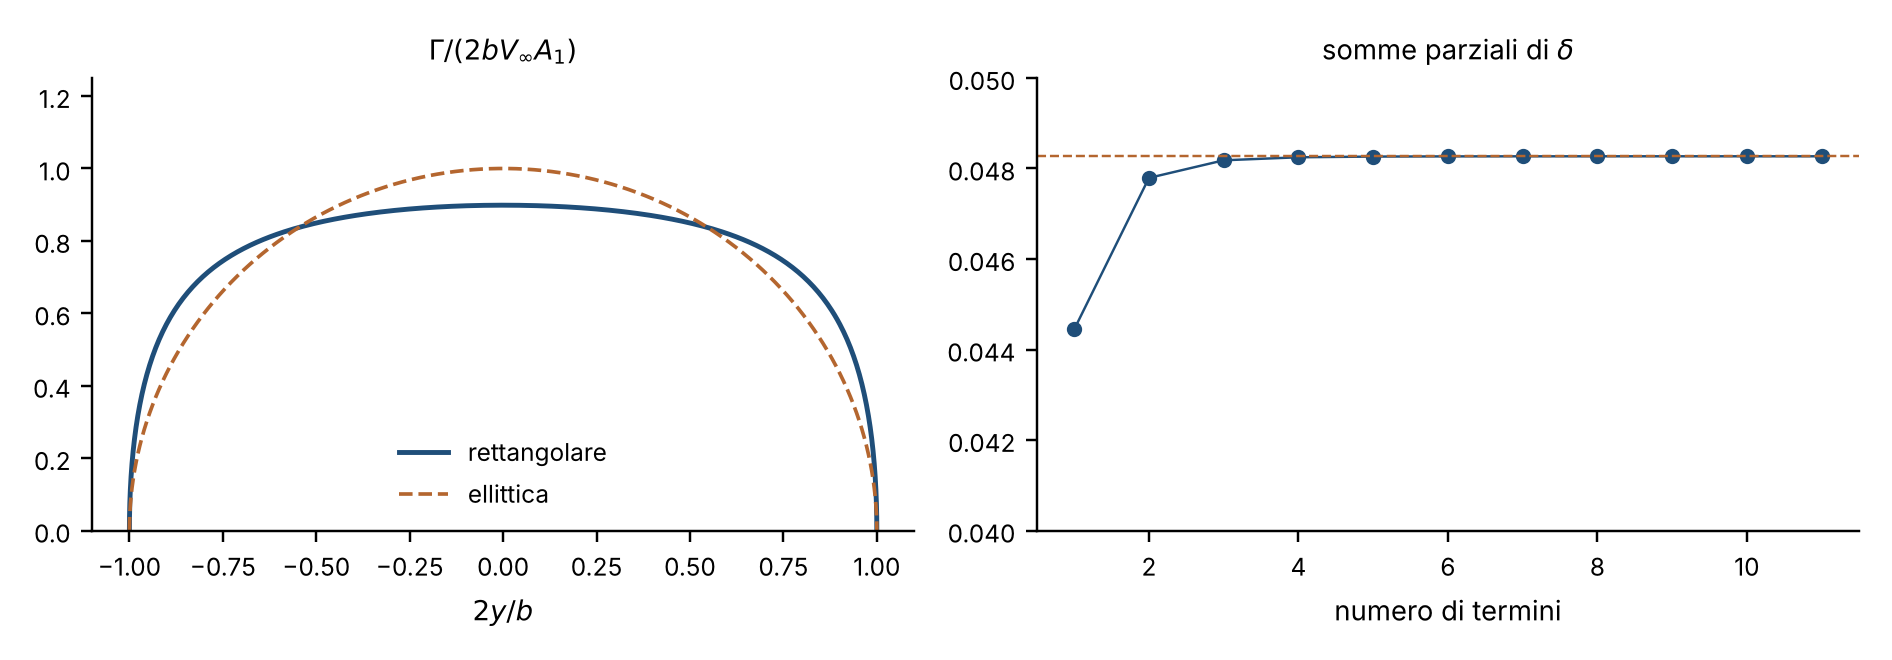
\includegraphics[width=\textwidth]{figure/resistenza_indotta.png}
\caption{A sinistra: la distribuzione di circolazione lungo l'apertura di un'ala
rettangolare con $AR=6$ (blu), confrontata con la distribuzione ellittica con la stessa
portanza (tratteggio rame). A destra: le somme parziali $\delta_{N}$ della serie
$\delta=\sum n(A_{n}/A_{1})^{2}$, crescenti e rapidamente convergenti, come deve accadere per
una serie convergente a termini non negativi (\texttt{python/fig\_resistenza\_indotta.py}).}
\label{fig:resistenza-indotta}
\end{figure}

\subsection{Approfondimento: prodotti infiniti e il prodotto di Wallis}
\label{subsec:prodotti-infiniti}

Come una serie è il limite delle somme dei suoi primi $n$ termini, così un \emph{prodotto
infinito} è il limite dei prodotti dei suoi primi $n$ fattori. Lo studio dei prodotti
infiniti si riconduce a quello delle serie, e conduce a una delle più antiche formule
per $\pi$.

\begin{definizione}[Prodotto infinito]\label{def:prodotto-infinito}
\index{prodotto infinito}
Sia $b_{k}>0$ per ogni $k\in\N$, e sia $p_{n}=b_{1}b_{2}\cdots b_{n}=\prod_{k=1}^{n}b_{k}$ il \emph{prodotto
parziale} $n$-esimo. Il prodotto infinito $\prod_{k=1}^{\infty}b_{k}$ si dice \emph{convergente} se
$p_{n}$ ha limite $P$ finito e \emph{positivo}, e allora si scrive $\prod_{k=1}^{\infty}b_{k}=P$; si
dice \emph{divergente} se $p_{n}\to+\infty$ oppure $p_{n}\to0$.
\end{definizione}

L'esclusione del limite $0$ è naturale. Passando ai logaritmi,
$\log p_{n}=\sum_{k=1}^{n}\log b_{k}$: se la serie $\sum\log b_{k}$ ha somma $L\in\R$, per la continuità
dell'esponenziale $p_{n}=e^{\log p_{n}}\to e^{L}>0$; viceversa, se $p_{n}\to P>0$, per la continuità del
logaritmo $\log p_{n}\to\log P$. Dunque \emph{il prodotto converge se e solo se converge la
serie dei logaritmi dei fattori}, e il caso $p_{n}\to0$ corrisponde a $\sum\log b_{k}=-\infty$. Come
per le serie, inoltre, se il prodotto converge i fattori $b_{n}=\frac{p_{n}}{p_{n-1}}$ tendono a
$\frac PP=1$: conviene scriverli nella forma $b_{k}=1+a_{k}$, con $a_{k}\to0$.

\begin{teorema}[Prodotti a fattori non minori di uno]\label{teo:prodotti-infiniti}
Sia $a_{k}\ge0$ per ogni $k$. Il prodotto $\prod_{k=1}^{\infty}(1+a_{k})$ converge se e solo se
converge la serie $\sum_{k=1}^{\infty}a_{k}$; altrimenti diverge a $+\infty$. Inoltre, dette $s_{n}$ e
$p_{n}$ le somme e i prodotti parziali,
\begin{equation}\label{eq:prodotti-stime}
  1+s_{n}\le p_{n}\le e^{s_{n}} \qquad\perogni n\in\N .
\end{equation}
\end{teorema}

\begin{schema}
\Ipotesi{$a_{k}\ge0$ per ogni $k$; \ $s_{n}=\sum_{k=1}^{n}a_{k}$, \ $p_{n}=\prod_{k=1}^{n}(1+a_{k})$.}
\Tesi{$1+s_{n}\le p_{n}\le e^{s_{n}}$; \ $\prod(1+a_{k})$ converge $\sse$ $\sum a_{k}<+\infty$; \
altrimenti $p_{n}\to+\infty$.}
\end{schema}

\begin{strategia}
Sviluppando il prodotto $(1+a_{1})\cdots(1+a_{n})$ si ottengono il termine $1$, tutti gli $a_{k}$ e
i loro prodotti, che sono non negativi: quindi $p_{n}\ge1+s_{n}$. La disuguaglianza
$1+x\le e^{x}$, applicata a ogni fattore, dà $p_{n}\le e^{a_{1}}\cdots e^{a_{n}}=e^{s_{n}}$. Le successioni $s_{n}$
e $p_{n}$ sono crescenti, e le due stime dicono che l'una è limitata se e solo se lo è
l'altra.
\end{strategia}

\begin{dimostrazione}
La prima delle \eqref{eq:prodotti-stime} si dimostra per induzione. Per $n=1$,
$p_{1}=1+a_{1}=1+s_{1}$. Se $p_{n}\ge1+s_{n}$, moltiplicando per $1+a_{n+1}>0$,
\[
  \begin{aligned}
  p_{n+1}&=p_{n}(1+a_{n+1})\ge(1+s_{n})(1+a_{n+1})\\
  &=1+s_{n+1}+s_{n}a_{n+1}\ge1+s_{n+1} .
  \end{aligned}
\]
Per la seconda, la \eqref{eq:exp-log-disuguaglianze} dà $0<1+a_{k}\le e^{a_{k}}$ per ogni $k$, e
moltiplicando membro a membro queste disuguaglianze tra numeri positivi
$p_{n}\le e^{a_{1}}e^{a_{2}}\cdots e^{a_{n}}=e^{s_{n}}$. La successione $p_{n}$ è crescente, perché
$p_{n+1}=p_{n}(1+a_{n+1})\ge p_{n}$, e $p_{n}\ge1$; per il \cref{teo:monotone} ha limite $P\in[1,+\infty]$.
Se $\sum a_{k}=s<+\infty$, allora $p_{n}\le e^{s_{n}}\le e^{s}$ e $P\in[1,e^{s}]$ è finito e positivo: il
prodotto converge. Se invece $s_{n}\to+\infty$, da $p_{n}\ge1+s_{n}$ e dal
\cref{teo:confronto-infinito} segue $p_{n}\to+\infty$.
\end{dimostrazione}

\begin{esempio}\label{es:prodotti-infiniti}
\begin{enumerate}[label=(\alph*)]
  \item Il prodotto $\prod_{k=1}^{\infty}\bigl(1+\frac1k\bigr)$ diverge: i fattori $\frac{k+1}k$ si semplificano «a
  cannocchiale» e $p_{n}=\frac21\cdot\frac32\cdots\frac{n+1}n=n+1$. La seconda delle \eqref{eq:prodotti-stime}
  diventa $n+1\le e^{H_{n}}$, cioè $H_{n}\ge\log(n+1)$: è la stima \eqref{eq:armonica-log}, che
  ritroviamo così per una quarta via.
  \item Il prodotto $\prod_{k=1}^{\infty}\bigl(1+\frac1{k^{2}}\bigr)$ converge, perché $\sum\frac1{k^{2}}$ converge, e per le
  \eqref{eq:prodotti-stime} il suo valore è compreso tra $1+\frac{\pi^{2}}6\approx2{,}64$ e
  $e^{\pi^{2}/6}\approx5{,}18$. (Il valore esatto è $\frac{e^{\pi}-e^{-\pi}}{2\pi}\approx3{,}68$.)
\end{enumerate}
\end{esempio}

Il prodotto infinito più celebre è quello di Wallis. I suoi fattori sono
$\frac{(2k)^{2}}{(2k-1)(2k+1)}=\frac{4k^{2}}{4k^{2}-1}=1+\frac1{4k^{2}-1}$, e poiché
$\frac1{4k^{2}-1}=\frac12\bigl(\frac1{2k-1}-\frac1{2k+1}\bigr)$, la serie $\sum\frac1{4k^{2}-1}$ è telescopica e
converge, con somma $\frac12$ (\cref{prop:serie-telescopica}): per il
\cref{teo:prodotti-infiniti} il prodotto converge, a un valore compreso tra $\frac32$ e
$e^{1/2}$. Il valore esatto viene dal calcolo integrale.

\begin{teorema}[Prodotto di Wallis]\label{teo:wallis}\index{prodotto di Wallis}
\begin{equation}\label{eq:wallis}
  \frac\pi2=\prod_{k=1}^{\infty}\frac{(2k)^{2}}{(2k-1)(2k+1)}
  =\frac21\cdot\frac23\cdot\frac43\cdot\frac45\cdot\frac65\cdot\frac67\cdots
\end{equation}
\end{teorema}

\begin{schema}
\Ipotesi{$I_{n}=\int_{0}^{\pi/2}\sen^{n}x\,dx$, con la formula di riduzione $I_{n}=\frac{n-1}nI_{n-2}$
per $n\ge2$ (\cref{es:wallis}); \ $W_{m}=\prod_{k=1}^{m}\frac{(2k)^{2}}{(2k-1)(2k+1)}$.}
\Tesi{$W_{m}\to\frac\pi2$.}
\end{schema}

\begin{strategia}
Iterando la formula di riduzione a partire da $I_{0}=\frac\pi2$ e $I_{1}=1$, l'integrale di indice
pari $I_{2m}$ contiene il fattore $\frac\pi2$ e quello di indice dispari $I_{2m+1}$ no, e il loro
rapporto risulta proprio $\frac\pi{2W_{m}}$. D'altra parte, poiché $0\le\sen x\le1$, le potenze
di $\sen x$ decrescono al crescere dell'esponente, e così i loro integrali:
$I_{2m+1}\le I_{2m}\le I_{2m-1}$. Questa catena intrappola il rapporto tra $1$ e $\frac{2m+1}{2m}$, che
tende a $1$, e il teorema dei carabinieri conclude.
\end{strategia}

\begin{dimostrazione}
Applicando $m$ volte la formula di riduzione (formalmente, per induzione su $m$),
\[
  I_{2m}=\frac{2m-1}{2m}\cdot\frac{2m-3}{2m-2}\cdots\frac12\cdot\frac\pi2 ,\qquad
  I_{2m+1}=\frac{2m}{2m+1}\cdot\frac{2m-2}{2m-1}\cdots\frac23\cdot1 .
\]
In particolare $I_{2m+1}>0$, e dividendo
\[
  \frac{I_{2m}}{I_{2m+1}}=\frac\pi2\prod_{k=1}^{m}\frac{2k-1}{2k}\cdot\prod_{k=1}^{m}\frac{2k+1}{2k}
  =\frac\pi2\prod_{k=1}^{m}\frac{(2k-1)(2k+1)}{(2k)^{2}}=\frac\pi{2W_{m}} .
\]
Per $x\in[0,\frac\pi2]$ si ha $0\le\sen x\le1$, e quindi
$\sen^{2m+1}x\le\sen^{2m}x\le\sen^{2m-1}x$; per il confronto tra integrali
(\cref{teo:confronto-integrali}), $I_{2m+1}\le I_{2m}\le I_{2m-1}$. Dividendo per $I_{2m+1}$ e usando la
formula di riduzione con $n=2m+1$, cioè $I_{2m-1}=\frac{2m+1}{2m}I_{2m+1}$, si ottiene
\[
  1\le\frac\pi{2W_{m}}\le\frac{2m+1}{2m}=1+\frac1{2m} \qquad\perogni m\in\N .
\]
Per il teorema dei carabinieri (\cref{teo:carabinieri}) $\frac\pi{2W_{m}}\to1$, e dunque
$W_{m}\to\frac\pi2$ (\cref{teo:operazioni-limiti}).
\end{dimostrazione}

L'ultima catena di disuguaglianze dice anche che
$0\le\frac\pi2-W_{m}\le\frac\pi2\bigl(1-\frac{2m}{2m+1}\bigr)=\frac\pi{2(2m+1)}$: l'errore è dell'ordine di $\frac1m$,
e la convergenza è lentissima. Il programma che segue mostra che ogni volta che il
numero dei fattori si moltiplica per dieci si guadagna una sola cifra esatta: il
prodotto $m\bigl(\frac\pi2-W_{m}\bigr)$ si stabilizza attorno a $\frac\pi8\approx0{,}3927$, cioè
$\frac\pi2-W_{m}\approx\frac\pi{8m}$, in accordo con la maggiorazione $\frac\pi{2(2m+1)}\approx\frac\pi{4m}$. Il
prodotto di Wallis non è dunque un metodo per calcolare $\pi$, ma un ponte tra il mondo
discreto dei prodotti di numeri interi e quello continuo degli integrali, che ritorna
nel calcolo delle probabilità e nella formula di Stirling per $n!$.

\needspace{14\baselineskip}
\begin{python}[La lenta convergenza del prodotto di Wallis]
import math

W = 1.0                                   # prodotto parziale W_m
for m in range(1, 10**6 + 1):
    W *= 4 * m * m / (4 * m * m - 1)
    if m in (10, 100, 1000, 10**4, 10**5, 10**6):
        err = math.pi / 2 - W
        print(f"m = {m:>7}: W_m = {W:.9f}  errore = {err:.2e}"
              f"  m*errore = {m * err:.5f}")
print(f"pi/2 = {math.pi / 2:.9f},  pi/8 = {math.pi / 8:.5f}")
\end{python}
\begin{risultato}
m =      10: W_m = 1.533851903  errore = 3.69e-02  m*errore = 0.36944
m =     100: W_m = 1.566893745  errore = 3.90e-03  m*errore = 0.39026
m =    1000: W_m = 1.570403873  errore = 3.92e-04  m*errore = 0.39245
m =   10000: W_m = 1.570757059  errore = 3.93e-05  m*errore = 0.39267
m =  100000: W_m = 1.570792400  errore = 3.93e-06  m*errore = 0.39270
m = 1000000: W_m = 1.570795934  errore = 3.93e-07  m*errore = 0.39270
pi/2 = 1.570796327,  pi/8 = 0.39270
\end{risultato}

\begin{notastorica}[Viète, Wallis, Brouncker, Newton]
Il primo prodotto infinito della storia è di François Viète (1593), che ottenne $\frac2\pi$
come prodotto di radici quadrate annidate studiando i poligoni regolari inscritti nel
cerchio. Il prodotto \eqref{eq:wallis} fu trovato da John Wallis, professore di geometria a
Oxford, nell'\emph{Arithmetica infinitorum} (1656), cercando l'area del quarto di cerchio,
cioè $\int_{0}^{1}\sqrt{1-x^{2}}\,dx=\frac\pi4$. Wallis sapeva calcolare gli integrali di $(1-x^{2})^{n}$ per
$n$ intero e ne «interpolò» il valore per $n=\frac12$, supponendo che la regolarità osservata
continuasse: un procedimento audace e senza dimostrazione, che il nostro
\cref{teo:wallis} giustifica a posteriori. Lord William Brouncker, futuro primo
presidente della Royal Society, trasformò il risultato in una frazione continua per
$\frac4\pi$, pubblicata nella stessa opera. Nell'inverno 1664--65 il giovane Isaac Newton
studiò l'\emph{Arithmetica infinitorum} e, applicando l'interpolazione di Wallis agli
integrali di $(1-t^{2})^{n}$ tra $0$ e un estremo variabile $x$, scoprì la serie binomiale
per esponenti frazionari (nota storica del \S\ref{sec:serie-taylor}). Circa ottant'anni
dopo il prodotto ricomparve come caso particolare di una scoperta di Eulero, la
scrittura del seno come prodotto infinito,
$\sen x=x\prod_{k=1}^{\infty}\bigl(1-\frac{x^{2}}{k^{2}\pi^{2}}\bigr)$, con cui nel 1734 egli ricavò la somma
$\frac{\pi^{2}}6$: con $x=\frac\pi2$ se ne ottiene proprio il prodotto di Wallis.
\end{notastorica}

%% ----------------------------------------------------------------------------
%%  §11.7  Serie alternate
%% ----------------------------------------------------------------------------
\section{Serie alternate}
\label{sec:serie-alternate}

Finora abbiamo studiato quasi esclusivamente serie a termini non negativi. Eliminiamo
questa restrizione, cominciando dalle \emph{serie alternate}\index{serie!alternata},
cioè le serie del tipo
\begin{equation}\label{eq:serie-alternata}
  \sum_{k=1}^{\infty}(-1)^{k-1}a_{k}=a_{1}-a_{2}+a_{3}-a_{4}+\dots+(-1)^{n-1}a_{n}+\cdots, \qquad a_{n}\ge0 ,
\end{equation}
in cui i termini cambiano segno a ogni passo. L'esempio tipico è la \emph{serie armonica
alternata}
\begin{equation}\label{eq:armonica-alternata}
  \sum_{k=1}^{\infty}\frac{(-1)^{k-1}}k=1-\frac12+\frac13-\frac14+\cdots ,
\end{equation}
che, a differenza della serie armonica, converge. Il meccanismo è visibile nella
\cref{fig:alternata}: ogni termine «corregge» il precedente con una correzione più
piccola, e le somme parziali oscillano attorno alla somma con oscillazioni sempre più
strette. Ci servirà un semplice lemma sulle successioni.

\begin{lemma}\label{lem:pari-dispari}
Se le estratte di indici pari $s_{2k}$ e di indici dispari $s_{2k+1}$ di una successione
$s_{n}$ convergono allo stesso limite $s$, allora $s_{n}\to s$.
\end{lemma}

\begin{schema}
\Ipotesi{$s_{2k}\to s$ \ e \ $s_{2k+1}\to s$ per $k\to+\infty$, con $s\in\R$.}
\Tesi{$s_{n}\to s$.}
\end{schema}

\begin{strategia}
Ogni indice $n$ è pari o dispari. Fissato $\epsilon>0$, le due estratte entrano
definitivamente nell'intorno $(s-\epsilon,s+\epsilon)$, ciascuna da un proprio indice in poi: basta
prendere il più grande dei due indici, tradotto in termini di $n$.
\end{strategia}

\begin{dimostrazione}
Sia $\epsilon>0$. Esistono $k_{1}$ e $k_{2}$ tali che $\abs{s_{2k}-s}<\epsilon$ per $k>k_{1}$ e
$\abs{s_{2k+1}-s}<\epsilon$ per $k>k_{2}$. Posto $\nu=2\max\{k_{1},k_{2}\}+1$, ogni $n>\nu$ è della forma
$2k$ con $k>k_{1}$ oppure $2k+1$ con $k>k_{2}$, e in entrambi i casi $\abs{s_{n}-s}<\epsilon$.
\end{dimostrazione}

\begin{teorema}[Criterio di Leibniz]\label{teo:leibniz}\index{criterio di Leibniz}
Sia $a_{n}\ge0$ una successione decrescente e infinitesima. Allora la serie alternata
\eqref{eq:serie-alternata} è convergente. Inoltre, detta $s$ la sua somma e $s_{n}$ la
somma parziale $n$-esima, si ha
\begin{equation}\label{eq:stima-leibniz}
  \abs{s_{n}-s}\le a_{n+1} \qquad\perogni n\in\N ,
\end{equation}
e la somma $s$ è compresa tra due somme parziali consecutive qualsiasi.
\end{teorema}

\begin{schema}
\Ipotesi{$a_{n}\ge0$; \ $a_{n+1}\le a_{n}$ per ogni $n$; \ $a_{n}\to0$.}
\Tesi{$\sum(-1)^{k-1}a_{k}$ converge; \ $\abs{s_{n}-s}\le a_{n+1}$.}
\end{schema}

\begin{strategia}
Separiamo le somme parziali di indice pari da quelle di indice dispari. Passando da
$s_{2k}$ a $s_{2k+2}$ si aggiunge $a_{2k+1}-a_{2k+2}\ge0$: le somme pari crescono. Passando da
$s_{2k-1}$ a $s_{2k+1}$ si aggiunge $-a_{2k}+a_{2k+1}\le0$: le somme dispari decrescono. Inoltre
ogni somma dispari supera ogni somma pari. Abbiamo due successioni monotòne e
limitate, una che sale e una che scende, la cui distanza $a_{2k+1}$ tende a zero: come in una
successione di intervalli incapsulati, convergono allo stesso limite, che è compreso tra
loro. La stima dell'errore segue proprio da questo «incapsulamento».
\end{strategia}

\begin{dimostrazione}
Per ogni $k\in\N$, poiché $a_{n}$ è decrescente,
\begin{align}
  s_{2k+2}&=s_{2k}+(a_{2k+1}-a_{2k+2})\ge s_{2k} , \label{eq:leibniz-pari}\\
  s_{2k+1}&=s_{2k-1}-(a_{2k}-a_{2k+1})\le s_{2k-1} . \label{eq:leibniz-dispari}
\end{align}
Dunque $s_{2}\le s_{4}\le s_{6}\le\cdots$ e $s_{1}\ge s_{3}\ge s_{5}\ge\cdots$. Inoltre
$s_{2k+1}-s_{2k}=a_{2k+1}\ge0$, e quindi
\begin{equation}\label{eq:leibniz-incapsulati}
  s_{2}\le s_{2k}\le s_{2k+1}\le s_{1} \qquad\perogni k\in\N .
\end{equation}
La successione $s_{2k}$ è crescente e limitata superiormente da $s_{1}$, la successione
$s_{2k+1}$ è decrescente e limitata inferiormente da $s_{2}$; per il teorema sulle successioni
monotòne (\cref{teo:monotone}) esse convergono, a limiti $s'$ e $s''$. Passando al limite
in $s_{2k+1}-s_{2k}=a_{2k+1}$ si ottiene $s''-s'=0$, perché $a_{n}\to0$. Per il
\cref{lem:pari-dispari} la serie converge, e la sua somma è $s=s'=s''$.

Per il teorema sulle successioni monotòne, inoltre, $s=\sup_{k}s_{2k}=\inf_{k}s_{2k+1}$, e quindi
$s_{2k}\le s\le s_{2k+1}$ e $s\le s_{2k-1}$ per ogni $k$. Ne segue
\begin{align*}
  0&\le s-s_{2k}\le s_{2k+1}-s_{2k}=a_{2k+1} ,\\
  0&\le s_{2k+1}-s\le s_{2k+1}-s_{2k+2}=a_{2k+2} ,
\end{align*}
cioè $\abs{s_{n}-s}\le a_{n+1}$ sia per $n=2k$ sia per $n=2k+1$; per $n=1$ la stessa disuguaglianza
segue da $s_{2}\le s\le s_{1}$. Le disuguaglianze $s_{2k}\le s\le s_{2k\pm1}$ dicono anche che $s$ è
compresa tra due somme parziali consecutive.
\end{dimostrazione}

La \eqref{eq:stima-leibniz} si enuncia spesso così: \emph{per una serie alternata che
verifica le ipotesi del criterio di Leibniz, l'errore che si commette sostituendo alla
somma la somma dei primi $n$ termini è maggiorato, in valore assoluto, dal primo termine
trascurato}. Si sa anche il segno dell'errore: è quello del primo termine trascurato.

\begin{esempio}[La serie armonica alternata]\label{es:armonica-alternata}
La successione $a_{n}=\frac1n$ è positiva, decrescente e infinitesima: la serie
\eqref{eq:armonica-alternata} converge. Quanti termini occorre sommare per avere
$\abs{s-s_{n}}\le\frac1{100}$? Per la \eqref{eq:stima-leibniz} basta che $a_{n+1}=\frac1{n+1}\le\frac1{100}$,
cioè $n\ge99$. Il valore della somma si ottiene dallo sviluppo del logaritmo: nel
\S\ref{sec:taylor-peano} abbiamo visto che
$\log(1+x)=\sum_{k=1}^{n}\frac{(-1)^{k-1}}kx^{k}+R(x)$ con $\abs{R(x)}\le\frac{x^{n+1}}{n+1}$ per $x\ge0$. Con
$x=1$, $\abs{\log2-s_{n}}\le\frac1{n+1}\to0$, e dunque
\begin{equation}\label{eq:somma-log2}
  1-\frac12+\frac13-\frac14+\dots=\log2=0{,}693147\ldots
\end{equation}
Allo stesso modo la serie di Leibniz \eqref{eq:serie-leibniz},
$1-\frac13+\frac15-\cdots=\frac\pi4$, verifica le ipotesi del criterio, e la stima
$\abs{s_{n}-\frac\pi4}\le\frac1{2n+1}$ ritrova quella del \cref{cap:taylor}.
\end{esempio}

\begin{attenzione}
L'ipotesi che $a_{n}$ sia \emph{decrescente} non si può omettere. Si consideri la serie
alternata con $a_{2j-1}=\frac1j$ e $a_{2j}=\frac1{4j^{2}}$:
\[
  1-\frac14+\frac12-\frac1{16}+\frac13-\frac1{36}+\cdots .
\]
I termini tendono a zero, ma non in modo monotòno. Le somme parziali di indice pari sono
$s_{2m}=\sum_{j=1}^{m}\bigl(\frac1j-\frac1{4j^{2}}\bigr)=H_{m}-\frac14\sum_{j=1}^{m}\frac1{j^{2}}$, che tende a $+\infty$
perché $H_{m}\to+\infty$ mentre $\sum\frac1{j^{2}}$ converge. Anche $s_{2m+1}=s_{2m}+\frac1{m+1}>s_{2m}$ tende a
$+\infty$, e per il \cref{lem:pari-dispari} (che vale, con la stessa dimostrazione e con gli
intorni di $+\infty$ al posto di quelli di $s$, anche per limiti infiniti) la serie diverge.
\end{attenzione}

\begin{figure}[htb]
\centering
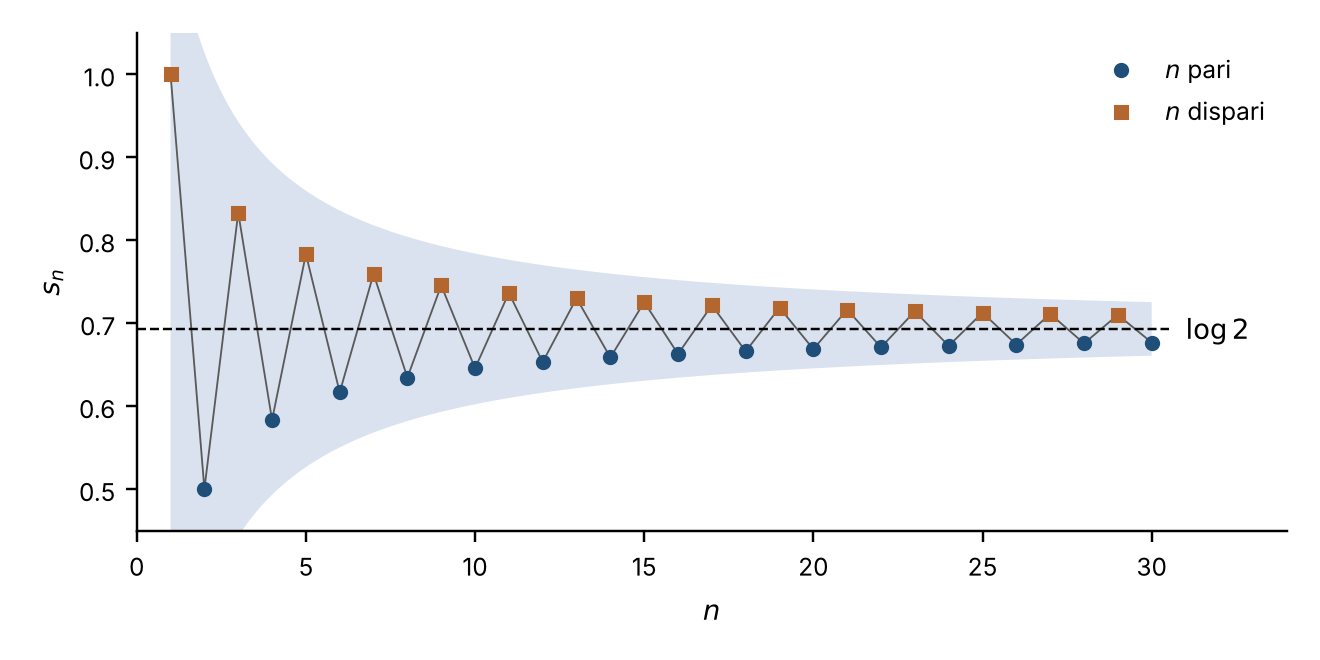
\includegraphics[width=\textwidth]{figure/alternata.png}
\caption{Le somme parziali della serie armonica alternata (punti) oscillano attorno alla
somma $\log2$: quelle di indice pari crescono, quelle di indice dispari decrescono, e la
somma è sempre compresa tra due somme consecutive. La fascia grigia ha semiampiezza
$a_{n+1}=\frac1{n+1}$, la stima dell'errore del criterio di Leibniz
(\texttt{python/fig\_alternata.py}).}
\label{fig:alternata}
\end{figure}

\needspace{10\baselineskip}
\begin{python}[La serie armonica alternata]
import math

s, err_max = 0.0, 0.0
for n in range(1, 10001):
    s += (-1)**(n - 1) / n
    errore = abs(s - math.log(2))
    err_max = max(err_max, errore * (n + 1))   # errore / a_(n+1)
    if n in (10, 99, 100, 1000, 10000):
        print(f"n = {n:5d}: s_n = {s:.8f}  errore = {errore:.2e}"
              f"  a_(n+1) = {1/(n+1):.2e}")
print(f"max di |s_n - log 2| / a_(n+1) = {err_max:.4f}  (<= 1)")
\end{python}
\begin{risultato}
n =    10: s_n = 0.64563492  errore = 4.75e-02  a_(n+1) = 9.09e-02
n =    99: s_n = 0.69817218  errore = 5.02e-03  a_(n+1) = 1.00e-02
n =   100: s_n = 0.68817218  errore = 4.98e-03  a_(n+1) = 9.90e-03
n =  1000: s_n = 0.69264743  errore = 5.00e-04  a_(n+1) = 9.99e-04
n = 10000: s_n = 0.69309718  errore = 5.00e-05  a_(n+1) = 1.00e-04
max di |s_n - log 2| / a_(n+1) = 0.6137  (<= 1)
\end{risultato}

%% ----------------------------------------------------------------------------
%%  §11.8  Convergenza assoluta
%% ----------------------------------------------------------------------------
\section{Convergenza assoluta}
\label{sec:convergenza-assoluta}

Per una serie a termini di segno qualsiasi, il primo passo è spesso studiare la serie
dei valori assoluti, che è a termini non negativi e alla quale si applicano tutti i
criteri del \S\ref{sec:criteri-convergenza}.

\begin{definizione}[Convergenza assoluta]\label{def:convergenza-assoluta}
\index{serie!assolutamente convergente}
La serie $\sum a_{k}$ si dice \emph{assolutamente convergente} se è convergente la serie dei
valori assoluti
\begin{equation}\label{eq:serie-valori-assoluti}
  \sum_{k=1}^{\infty}\abs{a_{k}}=\abs{a_{1}}+\abs{a_{2}}+\dots+\abs{a_{n}}+\cdots .
\end{equation}
\end{definizione}

Una serie convergente non è necessariamente assolutamente convergente: la serie armonica
alternata converge, ma la serie dei suoi valori assoluti è la serie armonica, che
diverge. Una serie convergente ma non assolutamente convergente si dice
\emph{semplicemente} (o \emph{condizionatamente}) convergente. Il viceversa, invece, vale.

\begin{teorema}[La convergenza assoluta implica la convergenza]
\label{teo:convergenza-assoluta}
Una serie assolutamente convergente è convergente, e
\begin{equation}\label{eq:disuguaglianza-serie}
  \Bigl|\sum_{k=1}^{\infty}a_{k}\Bigr|\le\sum_{k=1}^{\infty}\abs{a_{k}} .
\end{equation}
\end{teorema}

\needspace{9\baselineskip}
\begin{schema}
\Ipotesi{$\sum\abs{a_{k}}<+\infty$.}
\Tesi{$\sum a_{k}$ converge e $\abs{\sum a_{k}}\le\sum\abs{a_{k}}$.}
\end{schema}

\begin{strategia}
Non conosciamo la somma della serie, e quindi conviene un criterio che non la richieda:
quello di Cauchy. I blocchi di termini consecutivi della serie data sono, per la
disuguaglianza triangolare, più piccoli dei corrispondenti blocchi della serie dei valori
assoluti, che verificano la condizione di Cauchy perché questa serie converge. Daremo
anche una seconda dimostrazione, che riconduce il problema a serie a termini non
negativi.
\end{strategia}

\begin{dimostrazione}[Prima dimostrazione (con il criterio di Cauchy)]
Poiché $\sum\abs{a_{k}}$ converge, per il criterio di Cauchy (\cref{teo:cauchy-serie}), dato
$\epsilon>0$ esiste $\nu$ tale che $\sum_{k=n+1}^{n+p}\abs{a_{k}}<\epsilon$ per ogni $n>\nu$ e ogni $p\in\N$. Per gli
stessi indici, per la disuguaglianza triangolare,
\[
  \Bigl|\sum_{k=n+1}^{n+p}a_{k}\Bigr|\le\sum_{k=n+1}^{n+p}\abs{a_{k}}<\epsilon ,
\]
e quindi, ancora per il criterio di Cauchy, la serie $\sum a_{k}$ converge. Infine, per
ogni $n$, $\abs{\sum_{k=1}^{n}a_{k}}\le\sum_{k=1}^{n}\abs{a_{k}}$; passando al limite (il valore assoluto è
continuo e le disuguaglianze larghe si conservano) si ottiene la
\eqref{eq:disuguaglianza-serie}.
\end{dimostrazione}

\begin{dimostrazione}[Seconda dimostrazione (con il confronto)]
Per ogni $k$ si ha $0\le a_{k}+\abs{a_{k}}\le2\abs{a_{k}}$. La serie di termine generale $2\abs{a_{k}}$
converge, e per il criterio del confronto converge anche la serie a termini non negativi
$\sum(a_{k}+\abs{a_{k}})$. Allora, per la linearità (\cref{prop:linearita-serie}), converge
anche la serie
\[
  \sum_{k=1}^{\infty}a_{k}=\sum_{k=1}^{\infty}\bigl(a_{k}+\abs{a_{k}}\bigr)-\sum_{k=1}^{\infty}\abs{a_{k}} ,
\]
differenza di due serie convergenti. La \eqref{eq:disuguaglianza-serie} si dimostra come
nella prima dimostrazione.
\end{dimostrazione}

Applicando i criteri del \S\ref{sec:criteri-convergenza} alla serie dei valori assoluti si
ottengono criteri di convergenza per serie a termini di segno qualsiasi. Ad esempio, dai
criteri del rapporto e della radice:

\begin{corollario}\label{cor:rapporto-assoluto}
Sia $a_{n}\neq0$ e supponiamo che esista $\ell=\lim\frac{\abs{a_{n+1}}}{\abs{a_{n}}}$ oppure
$\ell=\lim\sqrt[n]{\abs{a_{n}}}$. Se $\ell<1$ la serie $\sum a_{k}$ converge assolutamente; se $\ell>1$ la
serie non converge.
\end{corollario}

\begin{schema}
\Ipotesi{$a_{n}\neq0$; \ $\frac{\abs{a_{n+1}}}{\abs{a_{n}}}\to\ell$ oppure $\sqrt[n]{\abs{a_{n}}}\to\ell$.}
\Tesi{$\ell<1\implica\sum a_{k}$ assolutamente convergente; \ $\ell>1\implica\sum a_{k}$ non converge.}
\end{schema}

\begin{strategia}
Si applicano i criteri del rapporto e della radice alla serie dei valori assoluti. Per
$\ell<1$ si conclude con il teorema appena dimostrato; per $\ell>1$ si riutilizza ciò che le
dimostrazioni di quei criteri hanno mostrato: il termine generale non tende a zero.
\end{strategia}

\begin{dimostrazione}
Se $\ell<1$, la serie $\sum\abs{a_{k}}$ converge per il \cref{teo:criterio-rapporto-serie} o per il
\cref{teo:criterio-radice}, e si applica il \cref{teo:convergenza-assoluta}. Se $\ell>1$, nelle
dimostrazioni di quei criteri abbiamo visto che $\abs{a_{n}}$ non tende a zero; allora neppure
$a_{n}$ tende a zero, e la serie non converge per il \cref{teo:condizione-necessaria}.
\end{dimostrazione}

\begin{esempio}\label{es:assoluta}
\begin{enumerate}[label=(\alph*)]
  \item $\sum\frac{\sen k}{k^{2}}$ converge assolutamente, perché $\frac{\abs{\sen k}}{k^{2}}\le\frac1{k^{2}}$. I segni dei
  suoi termini non seguono alcuno schema regolare: il criterio di Leibniz non sarebbe
  applicabile.
  \item La serie esponenziale $\sum\frac{x^{k}}{k!}$ converge assolutamente per \emph{ogni}
  $x\in\R$: il rapporto dei valori assoluti è $\frac{\abs x}{n+1}\to0$.
  \item $\sum\frac{(-1)^{k}}{\sqrt k}$ converge per il criterio di Leibniz, ma non assolutamente,
  perché $\sum\frac1{\sqrt k}$ diverge ($p=\frac12$).
\end{enumerate}
\end{esempio}

\subsection{Riordinare una serie}

In una somma finita l'ordine degli addendi è irrilevante. Per le serie la questione è
delicata, perché la somma è un limite, e il limite dipende dall'ordine in cui si
presentano le somme parziali. Un \emph{riordinamento} della serie $\sum a_{k}$ è una serie
$\sum a_{\sigma(k)}$, dove $\sigma:\N\to\N$ è una funzione biunivoca: gli stessi termini, ciascuno
preso una e una sola volta, in un ordine diverso.

\begin{teorema}[di Dirichlet]\label{teo:dirichlet-riordinamento}
\index{teorema!di Dirichlet sui riordinamenti}
Se la serie $\sum a_{k}$ è assolutamente convergente, ogni suo riordinamento è
assolutamente convergente e ha la stessa somma.
\end{teorema}

\begin{schema}
\Ipotesi{$\sum\abs{a_{k}}<+\infty$; \ $\sigma:\N\to\N$ biunivoca.}
\Tesi{$\sum a_{\sigma(k)}$ converge assolutamente e $\sum_{k=1}^{\infty}a_{\sigma(k)}=\sum_{k=1}^{\infty}a_{k}$.}
\end{schema}

\begin{strategia}
Per le serie a termini non negativi la somma è l'estremo superiore delle somme parziali,
e ogni somma parziale della serie riordinata è maggiorata da una somma parziale della
serie data (basta prendere abbastanza termini da includere tutti quelli usati): dunque la
somma riordinata non supera quella originale, e per simmetria vale anche il viceversa.
Il caso generale si riconduce a questo scrivendo ogni termine come differenza della sua
parte positiva e della sua parte negativa.
\end{strategia}

\begin{dimostrazione}
\emph{Primo passo: $a_{k}\ge0$.} Sia $s=\sum a_{k}$ e sia $t_{n}=\sum_{k=1}^{n}a_{\sigma(k)}$. Posto
$N=\max\{\sigma(1),\dots,\sigma(n)\}$, gli indici $\sigma(1),\dots,\sigma(n)$ sono distinti e compresi tra $1$ e $N$,
e poiché i termini sono non negativi $t_{n}\le\sum_{j=1}^{N}a_{j}\le s$. Dunque la serie riordinata, a
termini non negativi, converge (\cref{teo:serie-positive}) e la sua somma $t$ verifica
$t\le s$. Ma la serie data è a sua volta un riordinamento di quella riordinata (mediante
la funzione inversa $\sigma^{-1}$), e lo stesso ragionamento dà $s\le t$. Quindi $t=s$.

\emph{Secondo passo: caso generale.} Poniamo $a_{k}^{+}=\max\{a_{k},0\}$ e $a_{k}^{-}=\max\{-a_{k},0\}$, in modo
che $a_{k}=a_{k}^{+}-a_{k}^{-}$ e $\abs{a_{k}}=a_{k}^{+}+a_{k}^{-}$. Poiché $0\le a_{k}^{\pm}\le\abs{a_{k}}$, le serie $\sum a_{k}^{+}$ e
$\sum a_{k}^{-}$ convergono per il confronto. Per il primo passo, applicato alle serie
$\sum\abs{a_{k}}$, $\sum a_{k}^{+}$ e $\sum a_{k}^{-}$, i loro riordinamenti convergono alle stesse somme; in
particolare $\sum a_{\sigma(k)}$ converge assolutamente e, per la linearità,
\[
  \sum_{k=1}^{\infty}a_{\sigma(k)}=\sum_{k=1}^{\infty}a_{\sigma(k)}^{+}-\sum_{k=1}^{\infty}a_{\sigma(k)}^{-}
  =\sum_{k=1}^{\infty}a_{k}^{+}-\sum_{k=1}^{\infty}a_{k}^{-}=\sum_{k=1}^{\infty}a_{k} . \qedhere
\]
\end{dimostrazione}

Per le serie semplicemente convergenti la situazione è opposta, e sorprendente.

\begin{esempio}[Un riordinamento della serie armonica alternata]\label{es:riordinamento}
Sia $L=\log2=1-\frac12+\frac13-\frac14+\cdots$. Moltiplicando per $\frac12$ (\cref{prop:linearita-serie})
e intercalando degli zeri, il che non cambia né il carattere né la somma
(\cref{oss:termini-nulli}),
\[
  \tfrac12L=0+\tfrac12+0-\tfrac14+0+\tfrac16+0-\tfrac18+\cdots .
\]
Sommando termine a termine con la serie di $L$, ancora per la linearità,
\[
  \tfrac32L=1+0+\tfrac13-\tfrac12+\tfrac15+0+\tfrac17-\tfrac14+\cdots ,
\]
e, togliendo gli zeri (ancora per l'\cref{oss:termini-nulli}),
\begin{equation}\label{eq:riordinamento}
  1+\frac13-\frac12+\frac15+\frac17-\frac14+\frac19+\frac1{11}-\frac16+\dots=\frac32\log2 .
\end{equation}
Il primo membro contiene esattamente i termini della serie armonica alternata, ciascuno
una volta, in un ordine diverso (due positivi e un negativo): è un suo riordinamento, ma
la somma è aumentata del $50\%$ (\cref{fig:riordinamento}).
\end{esempio}

Il fenomeno è del tutto generale, come dimostrò Riemann; ci limitiamo a enunciare il
risultato e a descrivere l'idea della dimostrazione.

\begin{teorema}[di Riemann, senza dimostrazione]\label{teo:riemann-riordinamento}
\index{teorema!di Riemann sui riordinamenti}
Se la serie $\sum a_{k}$ è semplicemente convergente, per ogni $L\in\overline\R$ esiste un suo
riordinamento che ha somma $L$; esistono inoltre riordinamenti indeterminati.
\end{teorema}

\begin{schema}
\Ipotesi{$\sum a_{k}$ convergente; \ $\sum\abs{a_{k}}=+\infty$; \ $L\in\overline\R$.}
\Tesi{esiste $\sigma:\N\to\N$ biunivoca con $\sum_{k=1}^{\infty}a_{\sigma(k)}=L$; \ esistono
riordinamenti indeterminati.}
\end{schema}

\begin{strategia}[Idea della dimostrazione]
Le serie $\sum a_{k}^{+}$ delle parti positive e $\sum a_{k}^{-}$ delle parti negative sono entrambe
divergenti (se una convergesse, convergerebbe anche l'altra, e quindi la serie dei valori
assoluti), mentre $a_{k}\to0$. Per ottenere la somma $L\in\R$ si prendono termini positivi
finché la somma parziale supera $L$, poi termini negativi finché scende sotto $L$, e così
via: le risorse non si esauriscono mai, perché ciascuna delle due serie diverge, e le
oscillazioni attorno a $L$ sono maggiorate dagli ultimi termini usati, che tendono a zero.
\end{strategia}

Il programma che segue mette in pratica questo algoritmo.

\begin{figure}[htb]
\centering
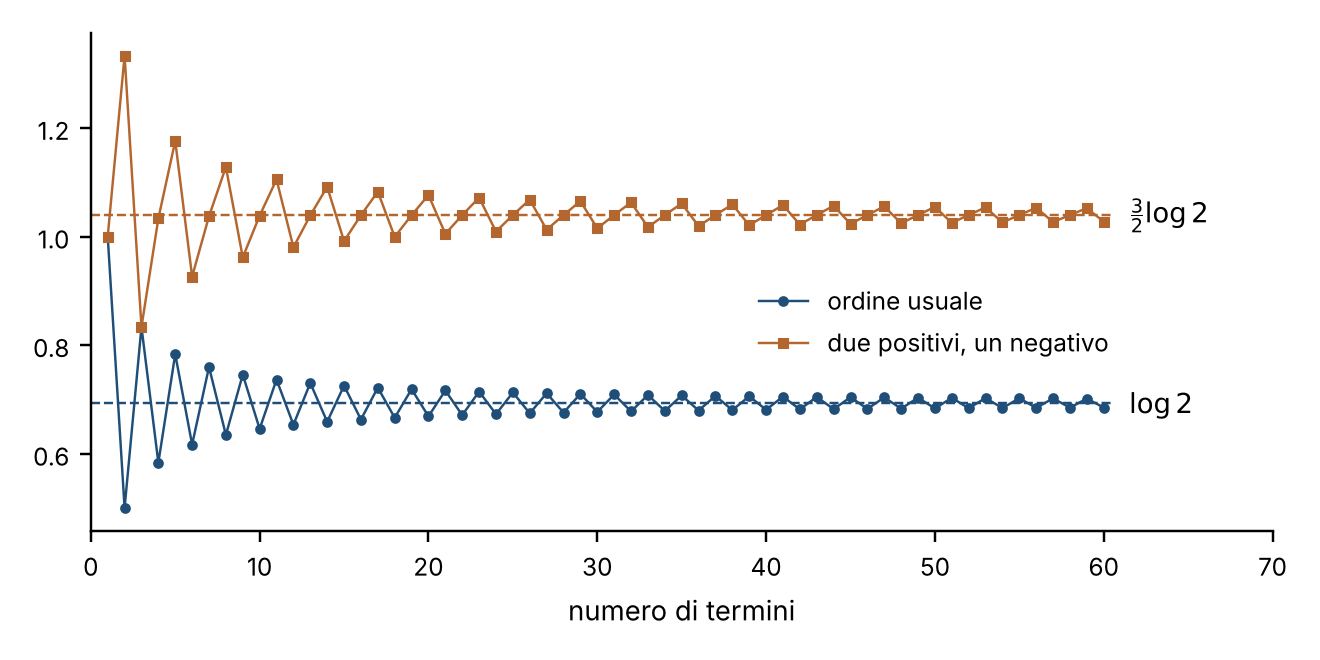
\includegraphics[width=\textwidth]{figure/riordinamento.png}
\caption{Somme parziali della serie armonica alternata nell'ordine usuale (blu), che
convergono a $\log2$, e del riordinamento \eqref{eq:riordinamento} con due termini positivi
e uno negativo (rame), che convergono a $\frac32\log2$. Gli stessi termini, sommati in un
ordine diverso, danno una somma diversa (\texttt{python/fig\_riordinamento.py}).}
\label{fig:riordinamento}
\end{figure}

\needspace{10\baselineskip}
\begin{python}[Riordinamenti della serie armonica alternata]
import math

def riordina(L, N):
    """Somma N termini di 1 - 1/2 + 1/3 - ... riordinati in modo
    che le somme parziali tendano a L (algoritmo di Riemann)."""
    s, p, q = 0.0, 1, 2          # prossimo dispari, prossimo pari
    for _ in range(N):
        if s <= L:
            s += 1 / p; p += 2   # termine positivo
        else:
            s -= 1 / q; q += 2   # termine negativo
    return s

s, p, q = 0.0, 1, 2              # due positivi e un negativo
for _ in range(100000):
    s += 1 / p + 1 / (p + 2) - 1 / q
    p, q = p + 4, q + 2
print(f"due +, un -:  {s:.6f}   (3/2) log 2 = {1.5*math.log(2):.6f}")
for L in (0.0, 1.0, math.pi):
    print(f"obiettivo L = {L:.6f}:  "
          f"somma = {riordina(L, 10**6):.6f}")
\end{python}
\begin{risultato}
due +, un -:  1.039718   (3/2) log 2 = 1.039721
obiettivo L = 0.000000:  somma = -0.000000
obiettivo L = 1.000000:  somma = 1.000000
obiettivo L = 3.141593:  somma = 3.141585
\end{risultato}

\begin{osservazione}
Il teorema di Dirichlet ha una conseguenza pratica: i termini di una serie
assolutamente convergente si possono raggruppare e riordinare nel modo più conveniente
senza alterare la somma, ad esempio sommando separatamente i termini positivi e quelli
negativi, o calcolando a parte certi blocchi di termini di cui si conosce la somma. Per
una serie semplicemente convergente, invece, l'ordine dei termini fa parte della
definizione stessa della serie. (Un'altra cosa è l'ordine in cui il calcolatore esegue
le addizioni di una somma parziale, che è una somma \emph{finita}: lì sommare dal termine
più piccolo al più grande riduce gli errori di arrotondamento, senza bisogno di alcun
teorema.)
\end{osservazione}

\begin{notastorica}[Cauchy, Dirichlet, Riemann]
Per tutto il Settecento le serie furono usate con grande disinvoltura, e talvolta con
risultati contraddittori. Fu Augustin-Louis Cauchy, nel \emph{Cours d'analyse} del 1821, a
fondarne la teoria sulla definizione di somma come limite delle somme parziali, con il
criterio che porta il suo nome (anticipato da Bernard Bolzano nel 1817), il criterio
della radice e quello di condensazione; quello del rapporto era già stato usato da d'Alembert. Nel 1837 Peter
Gustav Lejeune Dirichlet osservò che il valore di una serie semplicemente convergente
dipende dall'ordine dei termini e dimostrò che ciò non accade per le serie
assolutamente convergenti. Bernhard Riemann dimostrò il teorema che porta il suo nome nella
dissertazione di abilitazione sulle serie trigonometriche (1854), pubblicata postuma nel
1867.
\end{notastorica}

%% ----------------------------------------------------------------------------
%%  §11.9  Appendice: serie di Taylor
%% ----------------------------------------------------------------------------
\section{Appendice: serie di Taylor}
\label{sec:serie-taylor}

Sia $f$ una funzione derivabile infinite volte in un intorno di un punto $x_{0}$. La
formula di Taylor del \cref{cap:taylor} approssima $f$ con polinomi di grado $n$
arbitrario; è naturale chiedersi che cosa accada facendo tendere $n$ all'infinito.

\needspace{14\baselineskip}
\begin{definizione}[Serie di Taylor]\label{def:serie-taylor}\index{serie!di Taylor}
La serie
\begin{equation}\label{eq:serie-taylor}
  \sum_{k=0}^{\infty}\frac{f^{(k)}(x_{0})}{k!}(x-x_{0})^{k}
  =f(x_{0})+f'(x_{0})(x-x_{0})+\frac{f''(x_{0})}2(x-x_{0})^{2}+\cdots
\end{equation}
si chiama \emph{serie di Taylor} di $f$ con centro $x_{0}$ (\emph{serie di Mac Laurin} se
$x_{0}=0$). La funzione $f$ si dice \emph{sviluppabile in serie di Taylor} con centro $x_{0}$
se esiste $\delta>0$ tale che
\begin{equation}\label{eq:sviluppabile}
  f(x)=\sum_{k=0}^{\infty}\frac{f^{(k)}(x_{0})}{k!}(x-x_{0})^{k} \qquad\perogni x:\ \abs{x-x_{0}}<\delta .
\end{equation}
\end{definizione}

La somma parziale $n$-esima della serie di Taylor è il polinomio di Taylor $T_{n}(x)$, e
$f(x)=T_{n}(x)+R_{n}(x)$. Dunque, per un $x$ fissato, \emph{la serie di Taylor converge a
$f(x)$ se e solo se il resto $R_{n}(x)$ tende a zero per $n\to+\infty$}. Si noti che non basta
che la serie converga: deve convergere proprio a $f(x)$. Il resto di Peano, che descrive
$R_{n}$ per $x\to x_{0}$ con $n$ fissato, non dice nulla su questa domanda; servono le stime del
resto del \S\ref{sec:resto-integrale} e del \S\ref{sec:resto-lagrange}.

\begin{teorema}[Sviluppabilità con derivate equilimitate]\label{teo:sviluppabilita}
Sia $f$ derivabile infinite volte nell'intervallo $[x_{0}-\delta,x_{0}+\delta]$, con $\delta>0$, e
supponiamo che esista un numero $M$ tale che
\begin{equation}\label{eq:derivate-equilimitate}
  \abs{f^{(n)}(x)}\le M \qquad\perogni x\in[x_{0}-\delta,x_{0}+\delta],\ \perogni n\in\N .
\end{equation}
Allora $f$ è sviluppabile in serie di Taylor con centro $x_{0}$, e la \eqref{eq:sviluppabile}
vale per ogni $x\in[x_{0}-\delta,x_{0}+\delta]$.
\end{teorema}

\begin{schema}
\Ipotesi{$f\in C^{\infty}([x_{0}-\delta,x_{0}+\delta])$; \ $\abs{f^{(n)}}\le M$ per ogni $n$, con $M$
indipendente da $n$.}
\Tesi{$f(x)=\sum_{k=0}^{\infty}\frac{f^{(k)}(x_{0})}{k!}(x-x_{0})^{k}$ per ogni $x\in[x_{0}-\delta,x_{0}+\delta]$.}
\end{schema}

\begin{strategia}
Basta mostrare che $R_{n}(x)\to0$. La stima del resto (\cref{cor:stima-resto}) dà
$\abs{R_{n}(x)}\le M\frac{\delta^{n+1}}{(n+1)!}$, e il fattoriale al denominatore vince sulla potenza al
numeratore. È essenziale che $M$ non dipenda da $n$.
\end{strategia}

\begin{dimostrazione}
Fissato $x\in[x_{0}-\delta,x_{0}+\delta]$, per il \cref{cor:stima-resto} e l'ipotesi
\eqref{eq:derivate-equilimitate}, con $\abs{x-x_{0}}\le\delta$,
\[
  \abs{R_{n}(x)}\le M\,\frac{\abs{x-x_{0}}^{n+1}}{(n+1)!}\le M\,\frac{\delta^{n+1}}{(n+1)!} .
\]
Per la gerarchia degli infiniti (\cref{teo:gerarchia}) $\frac{\delta^{n+1}}{(n+1)!}\to0$ (se $\delta\le1$
basta maggiorare con $\frac1{(n+1)!}$), e quindi $R_{n}(x)\to0$, cioè $T_{n}(x)=f(x)-R_{n}(x)\to f(x)$.
\end{dimostrazione}

Si noti che la maggiorazione $M\frac{\delta^{n+1}}{(n+1)!}$ \emph{non dipende da $x$}: l'errore commesso
sostituendo $f$ con $T_{n}$ è piccolo, per $n$ grande, contemporaneamente in tutti i punti
dell'intervallo. È il fatto, osservato nel \cref{sec:taylor} per il seno
(\cref{fig:taylor-seno}), che i polinomi di Taylor di grado alto approssimano bene la
funzione su intervalli sempre più ampi.

\begin{notastorica}[Cauchy, Abel e la convergenza uniforme]
Nel \emph{Cours d'analyse} (1821) Cauchy enunciò un teorema in apparenza naturale: se una
serie di funzioni continue converge in ogni punto di un intervallo, la sua somma è
continua. Cinque anni dopo Niels Henrik Abel, nella memoria del 1826 sulla serie
binomiale di Newton, di cui studiava la convergenza anche per esponenti e variabile
complessi, osservò in nota che il teorema «ammette eccezioni»: la serie
$\sen x-\frac12\sen2x+\frac13\sen3x-\cdots$, i cui termini sono funzioni continue, converge per ogni
$x$ e ha somma $\frac x2$ per $-\pi<x<\pi$, ma per $x=\pi$ vale $0$: la somma ha un salto. Serie di
seni e coseni di questo tipo erano al centro della \emph{Théorie analytique de la chaleur}
di Joseph Fourier (1822, con risultati presentati già nel 1807), che vi sviluppava
funzioni qualsiasi, anche discontinue; la serie di Glauert \eqref{eq:glauert} appartiene
alla stessa famiglia. Al teorema di Cauchy manca l'ipotesi che l'errore commesso
troncando la serie sia piccolo \emph{contemporaneamente} in tutti i punti, come accade
nella stima del \cref{teo:sviluppabilita}: è la \emph{convergenza uniforme}. Intravista
negli anni Quaranta da Philipp Seidel e George Stokes, e usata da Cauchy stesso nel 1853
per correggere il proprio enunciato, essa divenne con Karl Weierstrass, che la usava già
nel 1841, uno strumento fondamentale dell'analisi.
\end{notastorica}

\begin{esempio}[Seno, coseno, esponenziale]\label{es:serie-elementari}
Le derivate di $\sen x$ e di $\cos x$ sono $\pm\sen x$ o $\pm\cos x$, e quindi sono limitate da
$M=1$ su qualunque intervallo. Per il \cref{teo:sviluppabilita}, con $x_{0}=0$ e $\delta$
arbitrario, e per gli sviluppi \eqref{eq:taylor-sen}, \eqref{eq:taylor-cos},
\begin{align}
  \sen x&=x-\frac{x^{3}}{3!}+\frac{x^{5}}{5!}-\dots=\sum_{k=0}^{\infty}(-1)^{k}\frac{x^{2k+1}}{(2k+1)!} , \label{eq:serie-seno}\\
  \cos x&=1-\frac{x^{2}}{2}+\frac{x^{4}}{4!}-\dots=\sum_{k=0}^{\infty}(-1)^{k}\frac{x^{2k}}{(2k)!} , \label{eq:serie-coseno}
\end{align}
per ogni $x\in\R$. Per l'esponenziale, $\abs{D^{n}e^{x}}=e^{x}\le e^{\delta}=M$ in $[-\delta,\delta]$; poiché $\delta$
è arbitrario,
\begin{equation}\label{eq:serie-esponenziale}
  e^{x}=1+x+\frac{x^{2}}{2!}+\dots+\frac{x^{n}}{n!}+\dots=\sum_{k=0}^{\infty}\frac{x^{k}}{k!} \qquad\perogni x\in\R ,
\end{equation}
che per $x=1$ ritrova la \eqref{eq:e-serie}. Le tre serie convergono assolutamente per ogni
$x$: l'esponenziale per l'\cref{es:assoluta}, il seno e il coseno per confronto con la
serie $\sum\frac{\abs x^{k}}{k!}$.
\end{esempio}

\needspace{12\baselineskip}
\begin{osservazione}[L'esponenziale definito da una serie]\label{oss:exp-serie}
Nel \cref{cap:numeri} avevamo annunciato una definizione alternativa delle potenze a
esponente reale. Eccola: si può \emph{definire} la funzione esponenziale mediante la
serie, $\exp x=\sum_{k=0}^{\infty}\frac{x^{k}}{k!}$, che converge per ogni $x$ reale, e poi porre
$a^{b}=\exp(b\log a)$ per $a>0$. Per la \eqref{eq:serie-esponenziale} e la relazione
$a^{b}=e^{b\log a}$ \eqref{eq:potenza-esponenziale}, questa definizione coincide con quella
data mediante l'estremo superiore. Molti testi seguono la strada inversa e costruiscono
tutta la teoria di esponenziali e logaritmi a partire dalla serie: la proprietà
fondamentale $\exp(x+y)=\exp x\cdot\exp y$ richiede allora di saper moltiplicare due serie
(il \emph{prodotto di Cauchy}), argomento dei corsi successivi.
\end{osservazione}

\subsection{Logaritmo e arcotangente}

Anche la serie geometrica è una serie di Taylor: per $f(x)=\frac1{1-x}$ si ha
$f^{(n)}(x)=\frac{n!}{(1-x)^{n+1}}$, cioè $\frac{f^{(n)}(0)}{n!}=1$, e il \cref{teo:serie-geometrica} dice che
$\frac1{1-x}=\sum_{k=0}^{\infty}x^{k}$ per $\abs x<1$. Il resto è esplicito,
$\frac1{1-x}-\sum_{k=0}^{n}x^{k}=\frac{x^{n+1}}{1-x}$, e integrandolo (con $-t$ o $-t^{2}$ al posto di $x$) abbiamo
ottenuto nel \S\ref{sec:taylor-peano} gli sviluppi del logaritmo e dell'arcotangente con
il resto in forma esplicita. Per queste funzioni le derivate non sono equilimitate, ma
il resto si può studiare direttamente.

\begin{proposizione}[Serie del logaritmo e dell'arcotangente]\label{prop:serie-log-arctg}
\begin{align}
  \log(1+x)&=\sum_{k=1}^{\infty}(-1)^{k-1}\frac{x^{k}}k=x-\frac{x^{2}}2+\frac{x^{3}}3-\cdots
  && (-1<x\le1), \label{eq:serie-log}\\
  \operatorname{arctg}x&=\sum_{k=0}^{\infty}(-1)^{k}\frac{x^{2k+1}}{2k+1}=x-\frac{x^{3}}3+\frac{x^{5}}5-\cdots
  && (-1\le x\le1). \label{eq:serie-arctg}
\end{align}
Per $\abs x>1$ entrambe le serie non convergono.
\end{proposizione}

\begin{schema}
\Ipotesi{$-1<x\le1$ per il logaritmo, $-1\le x\le1$ per l'arcotangente; \ $\abs x>1$ per
l'ultima affermazione.}
\Tesi{le somme parziali delle due serie tendono a $\log(1+x)$ e a $\operatorname{arctg}x$;
\ per $\abs x>1$ le serie non convergono.}
\end{schema}

\begin{strategia}
Per entrambe le funzioni il resto è stato ottenuto integrando il resto esplicito della
progressione geometrica, e ne conosciamo una maggiorazione: basta verificare che tende a
zero per $n\to+\infty$ quando $\abs x\le1$ (escluso $x=-1$ per il logaritmo, dove la funzione non
è definita). Per $\abs x>1$ si usa la condizione necessaria.
\end{strategia}

\begin{dimostrazione}
Per il logaritmo, nel \S\ref{sec:taylor-peano} abbiamo trovato
$\abs{R_{n}(x)}\le\frac{x^{n+1}}{n+1}$ per $0\le x\le1$ e $\abs{R_{n}(x)}\le\frac{\abs x^{n+1}}{(n+1)(1+x)}$ per $-1<x<0$; in
entrambi i casi $R_{n}(x)\to0$, perché $\abs x\le1$ e $\frac1{n+1}\to0$. Per l'arcotangente, la
\cref{prop:sviluppo-arctg} dà $\abs{R(x)}\le\frac{\abs x^{2n+3}}{2n+3}\to0$ per $\abs x\le1$. Se infine
$\abs x>1$, i termini $\frac{\abs x^{k}}k$ e $\frac{\abs x^{2k+1}}{2k+1}$ tendono a $+\infty$ (gerarchia degli
infiniti), e le serie non convergono per la condizione necessaria.
\end{dimostrazione}

Con $x=1$ si ritrovano le somme $\log2$ della serie armonica alternata e $\frac\pi4$ della
serie di Leibniz. Le due serie convergono però lentamente; per calcolare davvero $\log2$
conviene un'altra serie. Sottraendo dalla \eqref{eq:serie-log} la stessa formula con $-x$
al posto di $x$ (\cref{prop:linearita-serie}), per $\abs x<1$ i termini di grado pari si
elidono e
\begin{equation}\label{eq:serie-log-rapporto}
  \log\frac{1+x}{1-x}=2\Bigl(x+\frac{x^{3}}3+\frac{x^{5}}5+\cdots\Bigr)=2\sum_{k=0}^{\infty}\frac{x^{2k+1}}{2k+1} .
\end{equation}
Con $x=\frac13$ si ottiene $\frac{1+x}{1-x}=2$: la serie ha i termini dell'ordine di $9^{-k}$, e dieci
termini danno $\log2$ con un errore dell'ordine di $10^{-11}$, mentre dieci termini della
serie armonica alternata danno a stento la prima cifra decimale (errore $\approx5\cdot10^{-2}$). È lo stesso principio della formula di Machin
per $\pi$. Con il resto integrale, la \cref{prop:sviluppo-log-rapporto} del
\cref{cap:taylor} dà anche una stima esplicita dell'errore, ed è il punto di partenza per
costruire un'intera tavola di logaritmi.

\begin{osservazione}[Il raggio di convergenza]\label{oss:raggio-convergenza}
\index{raggio di convergenza}
Le serie di questo paragrafo sono \emph{serie di potenze} $\sum_{k=0}^{\infty}c_{k}x^{k}$ (con centro $0$;
per un centro $x_{0}$ basta scrivere $x-x_{0}$ al posto di $x$), e l'insieme degli $x$ in cui
convergono ha una struttura semplice. Se la serie converge in un punto $y\neq0$, i
termini $c_{k}y^{k}$ tendono a zero e sono quindi limitati, $\abs{c_{k}y^{k}}\le M$; per $\abs x<\abs y$
si ha allora $\abs{c_{k}x^{k}}\le M\abs{x/y}^{k}$, e per il confronto con una serie geometrica la
serie converge assolutamente in $x$ (\emph{lemma di Abel}). Posto
$r=\sup\{\abs y\tc\text{la serie converge in }y\}\in[0,+\infty]$, la serie converge dunque
assolutamente per $\abs x<r$ e, per definizione di $r$, non converge per $\abs x>r$; negli
estremi $x=\pm r$ può accadere di tutto. Il numero $r$ si chiama \emph{raggio di
convergenza}: nel campo complesso l'insieme $\abs z<r$ è un disco, e il nome viene di lì.

Quando esiste $L=\lim\frac{\abs{c_{k+1}}}{\abs{c_{k}}}$ (con $c_{k}\neq0$) oppure $L=\lim\sqrt[k]{\abs{c_{k}}}$, il
raggio si calcola con il \cref{cor:rapporto-assoluto}: per i termini $c_{k}x^{k}$ il limite
corrispondente vale $L\abs x$, e quindi $r=\frac1L$, con $r=+\infty$ se $L=0$ e $r=0$ se $L=+\infty$.
Così la serie esponenziale ha $r=+\infty$, quella del logaritmo $r=1$; per l'arcotangente,
che ha nulli i coefficienti di indice pari, si applica il criterio direttamente ai
termini non nulli, il cui rapporto tende a $x^{2}$, e si trova ancora $r=1$. La serie
$\sum\frac{x^{k}}k$ dell'\cref{es:serie-xk-su-k} ha $r=1$, converge in $-1$ e non in $1$.
Quando nessuno dei due limiti esiste, il raggio si calcola con il massimo limite
(\S\ref{subsec:massimo-minimo-limite}): vale sempre la \emph{formula di
Cauchy--Hadamard}\index{formula di Cauchy--Hadamard}
$\frac1r=\limsup_{k}\sqrt[k]{\abs{c_{k}}}$ (con le convenzioni $\frac10=+\infty$ e
$\frac1{+\infty}=0$, e il massimo limite $+\infty$ per le successioni non limitate
superiormente), che qui non dimostriamo.
\end{osservazione}

\subsection{Una funzione non sviluppabile}

Ci si potrebbe aspettare che ogni funzione derivabile infinite volte sia sviluppabile in
serie di Taylor. Non è così, e il controesempio, dovuto a Cauchy, è istruttivo.

\begin{proposizione}[Controesempio di Cauchy]\label{prop:cauchy-controesempio}
La funzione
\begin{equation}\label{eq:cauchy-controesempio}
  f(x)=\begin{cases} e^{-1/x^{2}} & \text{se } x\neq0,\\ 0 & \text{se } x=0 \end{cases}
\end{equation}
è derivabile infinite volte in $\R$, e $f^{(n)}(0)=0$ per ogni $n$. Dunque la sua serie di
Mac Laurin è identicamente nulla e converge a $f(x)$ soltanto per $x=0$: $f$ non è
sviluppabile in serie di Taylor con centro $0$.
\end{proposizione}

\begin{schema}
\Ipotesi{$f$ definita dalla \eqref{eq:cauchy-controesempio}.}
\Tesi{$f\in C^{\infty}(\R)$; \ $f^{(n)}(0)=0$ per ogni $n$; \ $f(x)\neq0=\sum\frac{f^{(k)}(0)}{k!}x^{k}$ per
$x\neq0$.}
\end{schema}

\begin{strategia}
Per $x\neq0$ le derivate si calcolano con le regole usuali, e per induzione hanno tutte
la forma $P(\frac1x)\,e^{-1/x^{2}}$, con $P$ polinomio. Il punto delicato è l'origine: lì la
funzione è «infinitamente piatta», perché $e^{-1/x^{2}}$ tende a zero più rapidamente di
qualunque potenza di $x$. Dimostreremo per induzione che ogni derivata esiste in $0$ e
vale $0$, calcolando il limite del rapporto incrementale.
\end{strategia}

\begin{dimostrazione}
\emph{Primo passo: un limite.} Per ogni intero $m\ge0$,
\begin{equation}\label{eq:piatta}
  \lim_{x\to0}\frac{e^{-1/x^{2}}}{\abs x^{m}}=0 .
\end{equation}
Infatti, posto $u=\frac1{x^{2}}\to+\infty$, il quoziente vale $u^{m/2}e^{-u}$, che tende a $0$ per la
\eqref{eq:hopital-potenza-exp} (per $m=0$ è ovvio) e il teorema sul limite delle funzioni
composte. Ne segue che $Q(\frac1x)\,e^{-1/x^{2}}\to0$ per $x\to0$, per ogni polinomio $Q$: è una
combinazione lineare di termini del tipo $\frac{e^{-1/x^{2}}}{x^{m}}$.

\emph{Secondo passo: le derivate per $x\neq0$.} Dimostriamo per induzione che per $x\neq0$
si ha $f^{(n)}(x)=P_{n}(\frac1x)\,e^{-1/x^{2}}$, con $P_{n}$ polinomio. Per $n=0$, $P_{0}=1$. Se la
formula vale per $n$, derivando con la regola del prodotto e quella delle funzioni
composte, e ricordando che $D\frac1x=-\frac1{x^{2}}$ e $D\bigl(-\frac1{x^{2}}\bigr)=\frac2{x^{3}}$,
\[
  f^{(n+1)}(x)=\Bigl[-\frac1{x^{2}}P_{n}'\Bigl(\frac1x\Bigr)+\frac2{x^{3}}P_{n}\Bigl(\frac1x\Bigr)\Bigr]e^{-1/x^{2}}
  =P_{n+1}\Bigl(\frac1x\Bigr)e^{-1/x^{2}} ,
\]
con $P_{n+1}(t)=-t^{2}P_{n}'(t)+2t^{3}P_{n}(t)$, che è un polinomio.

\emph{Terzo passo: le derivate in $0$.} Dimostriamo per induzione che $f^{(n)}(0)$ esiste e
vale $0$. Per $n=0$ è la definizione. Se $f^{(n)}(0)=0$, il rapporto incrementale di $f^{(n)}$
in $0$ è
\[
  \frac{f^{(n)}(x)-f^{(n)}(0)}{x}=\frac1x\,P_{n}\Bigl(\frac1x\Bigr)e^{-1/x^{2}} ,
\]
cioè $Q(\frac1x)e^{-1/x^{2}}$ con $Q(t)=tP_{n}(t)$, che tende a $0$ per il primo passo. Dunque
$f^{(n+1)}(0)=0$. In particolare ogni $f^{(n)}$ è derivabile in tutto $\R$, e quindi $f$ è
derivabile infinite volte. Infine la serie di Mac Laurin di $f$ ha tutti i coefficienti
nulli, e la sua somma è $0\neq e^{-1/x^{2}}=f(x)$ per ogni $x\neq0$.
\end{dimostrazione}

\begin{figure}[htb]
\centering
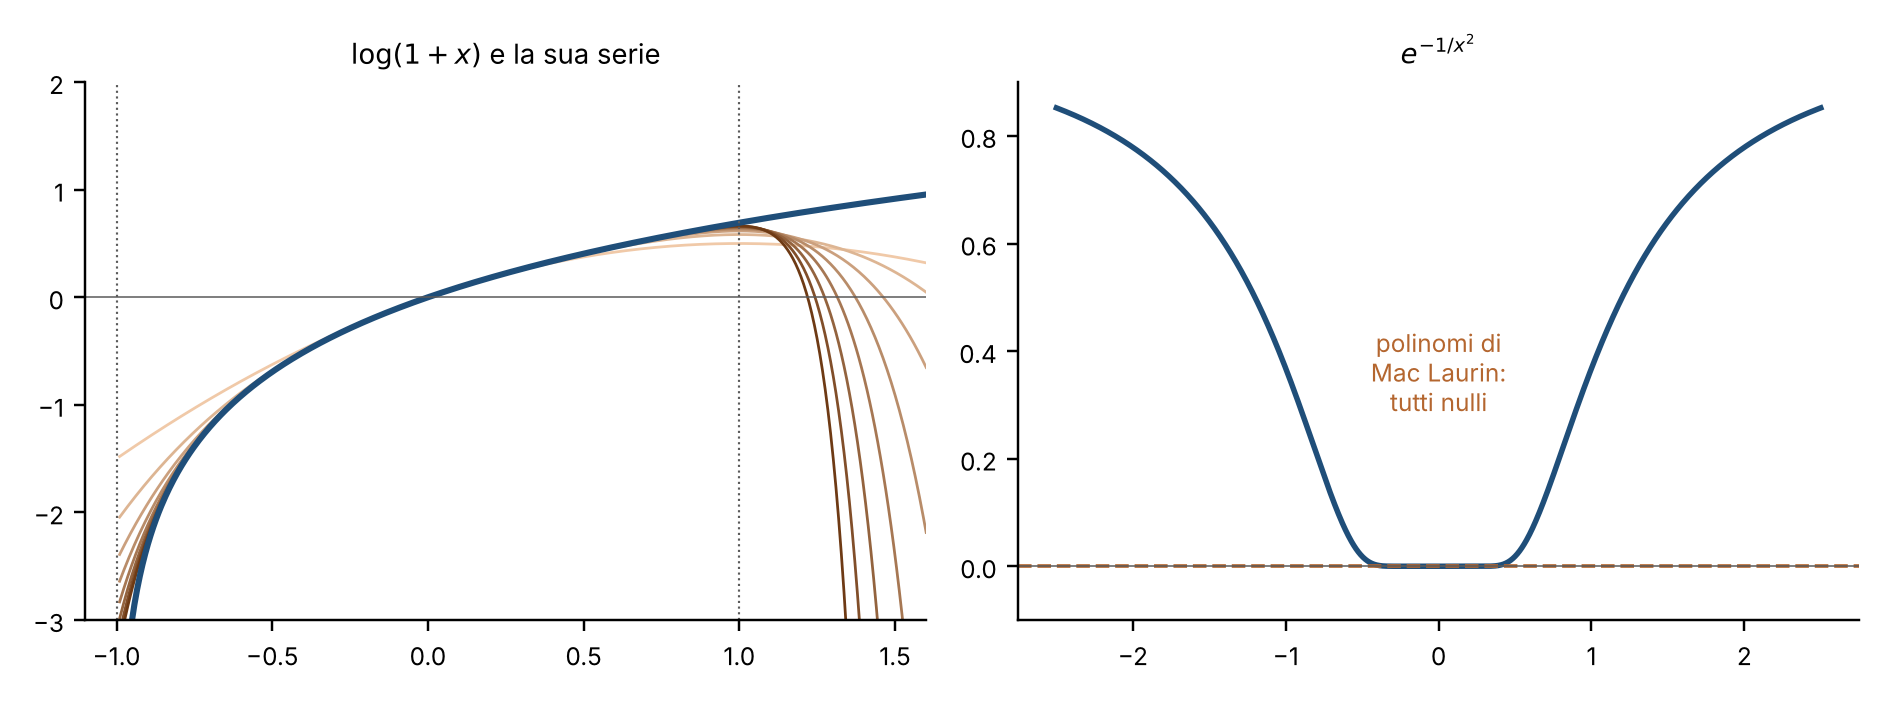
\includegraphics[width=\textwidth]{figure/serie_taylor.png}
\caption{A sinistra: $\log(1+x)$ (blu) e le somme parziali della sua serie di Mac Laurin di
grado $2,4,\dots,16$ (rame): in $(-1,1]$ esse convergono alla funzione, per $x>1$ si
allontanano. A destra: la funzione di Cauchy $e^{-1/x^{2}}$, così piatta nell'origine che tutti
i suoi polinomi di Mac Laurin sono nulli (\texttt{python/fig\_serie\_taylor.py}).}
\label{fig:serie-taylor}
\end{figure}

\subsection{La formula di Eulero}

Nel \cref{cap:complementi} abbiamo introdotto la notazione $e^{i\vartheta}=\cos\vartheta+i\sen\vartheta$
\eqref{eq:eulero}, promettendo di mostrare che si tratta in realtà di un teorema. Le serie
permettono di mantenere la promessa. Diciamo che una successione di numeri complessi
$z_{n}=x_{n}+iy_{n}$ converge a $z=x+iy$ se $x_{n}\to x$ e $y_{n}\to y$, e che una serie di numeri
complessi converge se convergono le sue somme parziali. Poiché la serie esponenziale
\eqref{eq:serie-esponenziale} converge per ogni $x$ reale, è naturale \emph{definire}
l'esponenziale di un numero complesso $z$ come
\begin{equation}\label{eq:esponenziale-complesso}
  e^{z}=\sum_{k=0}^{\infty}\frac{z^{k}}{k!} ,
\end{equation}
definizione che per $z$ reale coincide con l'esponenziale già nota. La serie converge per
ogni $z\in\mathbb C$. Infatti la parte reale e la parte immaginaria di un numero complesso non
superano in valore assoluto il suo modulo, e $\abs{z^{k}}=\abs z^{k}$ (per la
\eqref{eq:prodotto-trigonometrico}); quindi
$\bigl|\operatorname{Re}\frac{z^{k}}{k!}\bigr|\le\frac{\abs z^{k}}{k!}$ e $\bigl|\operatorname{Im}\frac{z^{k}}{k!}\bigr|\le\frac{\abs z^{k}}{k!}$. La serie
$\sum\frac{\abs z^{k}}{k!}$ converge, e per il confronto e il \cref{teo:convergenza-assoluta}
convergono le serie delle parti reali e delle parti immaginarie.

\begin{teorema}[Formula di Eulero]\label{teo:formula-eulero}\index{formula di Eulero}
Per ogni $\vartheta\in\R$ la serie $\sum_{k=0}^{\infty}\frac{(i\vartheta)^{k}}{k!}$ converge, e
\begin{equation}\label{eq:formula-eulero}
  e^{i\vartheta}=\sum_{k=0}^{\infty}\frac{(i\vartheta)^{k}}{k!}=\cos\vartheta+i\sen\vartheta .
\end{equation}
\end{teorema}

\begin{schema}
\Ipotesi{$\vartheta\in\R$; \ $e^{z}$ definito dalla \eqref{eq:esponenziale-complesso}; \ le serie
\eqref{eq:serie-seno} e \eqref{eq:serie-coseno}.}
\Tesi{$\sum_{k=0}^{\infty}\frac{(i\vartheta)^{k}}{k!}=\cos\vartheta+i\sen\vartheta$.}
\end{schema}

\begin{strategia}
Le potenze di $i$ valgono ciclicamente $1,i,-1,-i$: nella serie esponenziale calcolata in
$i\vartheta$, i termini di indice pari sono reali e riproducono, con i loro segni alterni, la serie
del coseno; quelli di indice dispari sono immaginari e riproducono la serie del seno.
Basta allora separare parte reale e parte immaginaria delle somme parziali e
riconoscere in esse le somme parziali delle due serie note.
\end{strategia}

\begin{dimostrazione}
Le potenze di $i$ si ripetono con periodo $4$: $i^{2m}=(-1)^{m}$ e $i^{2m+1}=(-1)^{m}i$. Quindi i
termini di indice pari della serie sono reali, $\frac{(i\vartheta)^{2m}}{(2m)!}=(-1)^{m}\frac{\vartheta^{2m}}{(2m)!}$, e
quelli di indice dispari sono immaginari puri,
$\frac{(i\vartheta)^{2m+1}}{(2m+1)!}=i\,(-1)^{m}\frac{\vartheta^{2m+1}}{(2m+1)!}$. La parte reale della somma parziale
$S_{n}=\sum_{k=0}^{n}\frac{(i\vartheta)^{k}}{k!}$ è allora la somma dei termini della serie del coseno
\eqref{eq:serie-coseno} con $2m\le n$, e la parte immaginaria è la somma dei termini della
serie del seno \eqref{eq:serie-seno} con $2m+1\le n$. Dette $C_{m}$ e $D_{m}$ le somme parziali
$m$-esime delle serie del coseno e del seno (con $m+1$ termini), si ha dunque
$\operatorname{Re}S_{2m}=\operatorname{Re}S_{2m+1}=C_{m}$ e $\operatorname{Im}S_{2m+1}=\operatorname{Im}S_{2m+2}=D_{m}$:
le estratte di indici pari e dispari di $\operatorname{Re}S_{n}$ tendono entrambe a $\cos\vartheta$, quelle di
$\operatorname{Im}S_{n}$ a $\sen\vartheta$, e per il \cref{lem:pari-dispari} si ha
$S_{n}\to\cos\vartheta+i\sen\vartheta$.
\end{dimostrazione}

Con $\vartheta=\pi$ si ottiene la celebre identità $e^{i\pi}+1=0$, che lega i cinque numeri più
importanti della matematica. Ora che $e^{i\vartheta}$ è definito dalla serie, la
\eqref{eq:prodotto-esponenziale} del \cref{cap:complementi},
$e^{i\vartheta}e^{i\vartheta'}=e^{i(\vartheta+\vartheta')}$, è un teorema: segue dalla formula di Eulero e dalle
formule di addizione, attraverso la \eqref{eq:prodotto-trigonometrico}. Per dimostrare
invece che $e^{z+w}=e^{z}e^{w}$ per $z$ e $w$ complessi qualsiasi occorre una regola per
moltiplicare due serie (il \emph{prodotto di Cauchy}), che si studia nei corsi
successivi.

\begin{python}[Serie di Taylor al lavoro]
import math

def exp_serie(x, N=100):
    """Somma dei primi N termini della serie esponenziale."""
    t, s = 1.0, 1.0
    for k in range(1, N):
        t *= x / k
        s += t
    return s

for x in (1.0, 5.0, -10.0, -20.0):
    print(f"x = {x:6.1f}: serie {exp_serie(x):.10e}   "
          f"exp {math.exp(x):.10e}")
print(f"e^-20 come 1/serie(20): {1 / exp_serie(20.0):.10e}")

lento = sum((-1)**(k - 1) / k for k in range(1, 11))
veloce = 2 * sum((1/3)**(2*k + 1) / (2*k + 1) for k in range(10))
print(f"log 2: lenta {lento:.6f}, veloce {veloce:.12f}, "
      f"esatto {math.log(2):.12f}")
print("e^(i pi) =", sum((1j * math.pi)**k / math.factorial(k)
                        for k in range(40)))
\end{python}
\begin{risultato}
x =    1.0: serie 2.7182818285e+00   exp 2.7182818285e+00
x =    5.0: serie 1.4841315910e+02   exp 1.4841315910e+02
x =  -10.0: serie 4.5399929670e-05   exp 4.5399929762e-05
x =  -20.0: serie 6.1475618289e-09   exp 2.0611536224e-09
e^-20 come 1/serie(20): 2.0611536224e-09
log 2: lenta 0.645635, veloce 0.693147180550, esatto 0.693147180560
e^(i pi) = (-1.0000000000000002+3.4586691443274427e-16j)
\end{risultato}

Il programma mette in luce un fatto importante per il calcolo numerico: per $x$ negativo
e grande in valore assoluto la serie esponenziale ha termini grandi di segno alterno, che
si cancellano quasi completamente, e la somma calcolata in virgola mobile perde tutte le
cifre significative. Il rimedio è calcolare $e^{x}=\frac1{e^{\abs x}}$ con la serie a termini
positivi: matematicamente le due strade sono equivalenti, numericamente no.

\needspace{10\baselineskip}
\begin{notastorica}[Le serie di potenze]
Isaac Newton scoprì nel 1665 la serie binomiale $(1+x)^{b}=\sum\binom bk x^{k}$ per esponenti $b$
qualsiasi, e ne fece lo strumento principale del suo calcolo; James Gregory (1671), Brook Taylor (1715) e
Colin Mac Laurin (1742) diedero il metodo generale per ottenere la serie di una funzione dalle
sue derivate. Eulero, nell'\emph{Introductio in analysin infinitorum} (1748), fondò sulle
serie di potenze la teoria delle funzioni elementari, ricavando tra l'altro la formula
che porta il suo nome. Per tutto il Settecento si ritenne, con Lagrange, che ogni funzione
«ragionevole» fosse uguale alla propria serie di Taylor; il controesempio di Cauchy, del
1823, mostrò che la derivabilità infinita non basta. Le funzioni sviluppabili in serie di
Taylor in un intorno di ogni punto si chiamano oggi \emph{analitiche}, e il loro studio,
che si svolge in modo naturale nel campo complesso, è uno dei capitoli più belli
dell'analisi.
\end{notastorica}

%% ----------------------------------------------------------------------------
%%  §11.10  Esercizi di riepilogo
%% ----------------------------------------------------------------------------
\section{Esercizi di riepilogo}
\label{sec:esercizi-cap11}

Come nei capitoli precedenti, ogni soluzione è accompagnata da una nota sulla
\emph{scelta logica} che la guida.

\needspace{8\baselineskip}
\subsection*{Somme di serie}

\begin{esercizio}
Calcolare $\displaystyle\sum_{k=1}^{\infty}\frac1{k(k+2)}$.
\begin{soluzione}
Decomponendo in fratti semplici, $\frac1{k(k+2)}=\frac12\bigl(\frac1k-\frac1{k+2}\bigr)$. Posto
$b_{k}=\frac1k+\frac1{k+1}$, si ha $b_{k}-b_{k+1}=\frac1k-\frac1{k+2}$, e per la \cref{prop:serie-telescopica}
$\sum_{k=1}^{\infty}\bigl(\frac1k-\frac1{k+2}\bigr)=b_{1}-\lim b_{n}=1+\frac12=\frac32$. Per la linearità la somma
cercata è $\frac34$. \emph{Scelta logica:} quando il termine generale è una funzione razionale,
la decomposizione in fratti semplici può rivelare una struttura telescopica; qui i
termini si elidono «a distanza due», e il trucco è raggruppare due addendi consecutivi
in $b_{k}$.
\end{soluzione}
\end{esercizio}

\begin{esercizio}
Studiare la serie $\sum_{k=1}^{\infty}\log\bigl(1+\frac1k\bigr)$.
\begin{soluzione}
Si ha $\log\bigl(1+\frac1k\bigr)=\log(k+1)-\log k=b_{k}-b_{k+1}$ con $b_{k}=-\log k$: per la
\cref{prop:serie-telescopica}, $s_{n}=\log(n+1)$, e poiché $b_{n}\to-\infty$ la serie diverge a
$+\infty$. In alternativa: $\log\bigl(1+\frac1n\bigr)\sim\frac1n$, e il confronto asintotico
(\cref{cor:confronto-asintotico}) con la serie armonica dà la divergenza.
\emph{Scelta logica:} il termine generale tende a zero, ma la condizione necessaria non
basta; due strade indipendenti (somma esplicita, parte principale) conducono alla stessa
conclusione.
\end{soluzione}
\end{esercizio}

\begin{esercizio}
Calcolare $\displaystyle\sum_{k=1}^{\infty}\frac{2^{k}+3^{k}}{6^{k}}$.
\begin{soluzione}
Il termine generale è $\bigl(\frac13\bigr)^{k}+\bigl(\frac12\bigr)^{k}$. Per la \eqref{eq:geometrica-generale}
con $m=1$, $\sum_{k\ge1}\bigl(\frac13\bigr)^{k}=\frac{1/3}{1-1/3}=\frac12$ e $\sum_{k\ge1}\bigl(\frac12\bigr)^{k}=1$; per la linearità
la somma è $\frac32$. \emph{Scelta logica:} si spezza il termine generale in somma di termini
geometrici; la linearità è lecita perché entrambe le serie convergono.
\end{soluzione}
\end{esercizio}

\begin{esercizio}
Per quali $x>0$ converge la serie $\sum_{k=0}^{\infty}(\log x)^{k}$? Calcolarne la somma.
\begin{soluzione}
È una serie geometrica di ragione $\log x$: converge se e solo se $\abs{\log x}<1$, cioè
$\frac1e<x<e$, e la somma è $\frac1{1-\log x}$. Per $x\ge e$ diverge, per $0<x\le\frac1e$ è indeterminata.
\emph{Scelta logica:} riconoscere una serie geometrica «travestita» è il primo passo di
fronte a una serie i cui termini sono potenze di un'unica espressione.
\end{soluzione}
\end{esercizio}

\begin{esercizio}
Calcolare $\displaystyle\sum_{k=0}^{\infty}\frac k{k!}$ e $\displaystyle\sum_{k=0}^{\infty}\frac{k^{2}}{k!}$.
\begin{soluzione}
Per $k\ge1$, $\frac k{k!}=\frac1{(k-1)!}$; il termine con $k=0$ è nullo. Quindi
$\sum_{k=0}^{\infty}\frac k{k!}=\sum_{j=0}^{\infty}\frac1{j!}=e$ per la \eqref{eq:e-serie} (con $j=k-1$). Analogamente
$\frac{k^{2}}{k!}=\frac k{(k-1)!}=\frac{(k-1)+1}{(k-1)!}$, e per $k\ge2$ si ha $\frac{k-1}{(k-1)!}=\frac1{(k-2)!}$; dunque
$\sum_{k=0}^{\infty}\frac{k^{2}}{k!}=\sum_{j=0}^{\infty}\frac1{j!}+\sum_{j=0}^{\infty}\frac1{j!}=2e$. \emph{Scelta logica:} semplificando il
fattoriale e cambiando indice ci si riconduce alla serie esponenziale; la linearità è
lecita perché tutte le serie coinvolte convergono.
\end{soluzione}
\end{esercizio}

\needspace{8\baselineskip}
\subsection*{Criteri di convergenza}

\begin{esercizio}\label{es:carattere}
Studiare il carattere delle serie
(a) $\sum\frac{k+1}{k^{3}+2}$; \ (b) $\sum\frac1{\sqrt{k(k+1)}}$; \ (c) $\sum\frac{k^{2}}{3^{k}}$; \
(d) $\sum\frac{k!}{(2k)!}$; \ (e) $\sum\bigl(1-\frac1k\bigr)^{k^{2}}$; \ (f) $\sum_{k\ge2}\frac1{\log k}$.
\begin{soluzione}
(a) Converge: $n^{2}\cdot\frac{n+1}{n^{3}+2}\to1$, criterio degli infinitesimi con $p=2$.
(b) Diverge: $n\cdot\frac1{\sqrt{n(n+1)}}\to1$, con $p=1$.
(c) Converge per il criterio del rapporto: $\frac{(n+1)^{2}}{3^{n+1}}\cdot\frac{3^{n}}{n^{2}}\to\frac13$.
(d) Converge per il criterio del rapporto: $\frac{(n+1)!}{(2n+2)!}\cdot\frac{(2n)!}{n!}=\frac{n+1}{(2n+1)(2n+2)}\to0$.
(e) Converge per il criterio della radice: $\sqrt[n]{a_{n}}=\bigl(1-\frac1n\bigr)^{n}\to\frac1e<1$
(\cref{teo:e-generalizzato}).
(f) Diverge per il confronto: $\log k<k$, e quindi $\frac1{\log k}>\frac1k$.
\emph{Scelta logica:} il criterio si sceglie guardando la forma del termine generale:
potenze di $n$ (confronto, infinitesimi), esponenziali e fattoriali (rapporto), potenze
con esponente $n$ (radice).
\end{soluzione}
\end{esercizio}

\needspace{7\baselineskip}
\begin{esercizio}
Per quali $\alpha>0$ converge la serie $\sum_{k=1}^{\infty}\bigl(e^{1/k^{\alpha}}-1\bigr)$?
\begin{soluzione}
I termini sono positivi. Dallo sviluppo $e^{t}-1=t+o(t)$ con $t=\frac1{n^{\alpha}}\to0$ si ha
$e^{1/n^{\alpha}}-1\sim\frac1{n^{\alpha}}$, e per il confronto asintotico la serie ha lo stesso carattere
dell'armonica generalizzata con $p=\alpha$: converge se e solo se $\alpha>1$. \emph{Scelta logica:}
la parte principale del termine generale riduce ogni serie di questo tipo a una serie
armonica generalizzata.
\end{soluzione}
\end{esercizio}

\begin{esercizio}
Quanti termini della serie $\sum\frac1{k^{3}}$ occorre sommare per avere la somma con un
errore inferiore a $10^{-4}$?
\begin{soluzione}
Per la \eqref{eq:resto-integrale-serie} con $f(x)=\frac1{x^{3}}$, il resto verifica
$R_{n}\le\int_{n}^{+\infty}\frac{dx}{x^{3}}=\frac1{2n^{2}}$. Basta $\frac1{2n^{2}}<10^{-4}$, cioè $n^{2}>5000$, $n\ge71$. La
stima dal basso $R_{n}\ge\frac1{2(n+1)^{2}}$ mostra che non si può fare molto meglio: per $n=60$
l'errore è certamente maggiore di $10^{-4}$. \emph{Scelta logica:} per le serie a termini
positivi e decrescenti il criterio dell'integrale fornisce non soltanto il carattere, ma
anche una stima del resto dall'alto e dal basso.
\end{soluzione}
\end{esercizio}

\needspace{8\baselineskip}
\subsection*{Serie a segni alterni e convergenza assoluta}

\begin{esercizio}
Dimostrare che $\sum_{k=1}^{\infty}(-1)^{k}\frac k{k^{2}+1}$ converge, ma non assolutamente.
\begin{soluzione}
La funzione $g(x)=\frac x{x^{2}+1}$ ha derivata $g'(x)=\frac{1-x^{2}}{(x^{2}+1)^{2}}\le0$ per $x\ge1$: la
successione $a_{n}=g(n)$ è decrescente, positiva e infinitesima, e la serie converge per il
criterio di Leibniz. La serie dei valori assoluti diverge, perché $\frac n{n^{2}+1}\sim\frac1n$.
\emph{Scelta logica:} la monotonia di una successione definita da una funzione si
verifica comodamente con il segno della derivata.
\end{soluzione}
\end{esercizio}

\begin{esercizio}
Calcolare $\sum_{k=1}^{\infty}\frac{(-1)^{k-1}}{k^{3}}$ con un errore inferiore a $10^{-3}$.
\begin{soluzione}
La serie verifica le ipotesi del criterio di Leibniz, e per la \eqref{eq:stima-leibniz}
basta $\frac1{(n+1)^{3}}\le10^{-3}$, cioè $n+1\ge10$. La somma dei primi $9$ termini è
$s_{9}\approx0{,}90212$, e la somma vera è compresa tra $s_{10}=s_{9}-10^{-3}$ e $s_{9}$; poiché i termini sono
strettamente decrescenti, essa è diversa da entrambi (le estratte pari e dispari sono
strettamente monotòne), e l'errore è strettamente minore di $10^{-3}$. Il valore è
$0{,}901543\ldots$ \emph{Scelta logica:} la serie converge anche assolutamente, ma per la
stima dell'errore il criterio di Leibniz è molto più preciso di quello dell'integrale
applicato alla serie dei valori assoluti.
\end{soluzione}
\end{esercizio}

\begin{esercizio}\label{es:serie-xk-su-k}
Determinare gli $x\in\R$ per cui converge la serie $\sum_{k=1}^{\infty}\frac{x^{k}}k$, e calcolarne la
somma.
\begin{soluzione}
Il rapporto dei valori assoluti è $\frac{\abs x\,n}{n+1}\to\abs x$: per il \cref{cor:rapporto-assoluto}
la serie converge assolutamente se $\abs x<1$ e non converge se $\abs x>1$. Per $x=1$ è la
serie armonica, divergente; per $x=-1$ è l'opposto della serie armonica alternata,
convergente. Dunque la serie converge se e solo se $-1\le x<1$, e, per la \eqref{eq:serie-log}
con $-x$ al posto di $x$, la somma è $-\log(1-x)$. \emph{Scelta logica:} il criterio del
rapporto decide all'interno e all'esterno dell'intervallo $(-1,1)$, ma non agli estremi,
dove $\ell=1$: lì servono considerazioni specifiche.
\end{soluzione}
\end{esercizio}

\needspace{8\baselineskip}
\subsection*{Applicazioni}

\begin{esercizio}[Resistenza indotta di un'ala non ellittica]
Per un'ala simmetrica i coefficienti di Glauert valgono $\frac{A_{3}}{A_{1}}=0{,}05$, $\frac{A_{5}}{A_{1}}=0{,}01$,
e i successivi sono trascurabili. Stimare l'aumento percentuale della resistenza indotta
rispetto all'ala ellittica con la stessa portanza e lo stesso allungamento.
\begin{soluzione}
Per la \eqref{eq:resistenza-indotta}, $\delta\approx3\cdot0{,}05^{2}+5\cdot0{,}01^{2}=0{,}0075+0{,}0005=0{,}008$: la
resistenza indotta è maggiore di circa lo $0{,}8\%$. Poiché la serie è a termini non
negativi, trascurare i termini successivi porta a una stima \emph{per difetto} di $\delta$.
\emph{Scelta logica:} in una serie a termini non negativi ogni somma parziale è un
minorante della somma; il segno dell'errore di troncamento è quindi noto.
\end{soluzione}
\end{esercizio}

\begin{esercizio}[Un rimbalzo smorzato]
Un corpo lasciato cadere da un'altezza $h_{0}$ rimbalza ogni volta fino a un'altezza pari a
una frazione $r<1$ della precedente. Calcolare lo spazio totale percorso e la durata
totale del moto, trascurando la resistenza dell'aria e la durata degli urti.
\begin{soluzione}
Lo spazio è $h_{0}+2rh_{0}+2r^{2}h_{0}+\dots=h_{0}+2h_{0}\frac r{1-r}=h_{0}\frac{1+r}{1-r}$. Il tempo di caduta da
un'altezza $h$ è $\sqrt{2h/g}$, e quindi una salita e una discesa dall'altezza $r^{k}h_{0}$ durano
$2\sqrt{2h_{0}/g}\,(\sqrt r)^{k}$. La durata totale è
$t_{0}+2t_{0}\sum_{k\ge1}(\sqrt r)^{k}=t_{0}\frac{1+\sqrt r}{1-\sqrt r}$, con $t_{0}=\sqrt{2h_{0}/g}$: infiniti rimbalzi in
un tempo finito (il numero $\sqrt r$ è il coefficiente di restituzione dell'urto; gli
infiniti rimbalzi sono naturalmente un'idealizzazione del modello). Con $h_{0}=1$~m e
$r=0{,}64$ lo spazio è $4{,}56$~m e la durata
$9t_{0}\approx4{,}06$~s. \emph{Scelta logica:} ogni grandezza che si riduce a ogni passo di un
fattore costante dà luogo a una serie geometrica; spazio e tempo sono due serie
geometriche di ragioni diverse, $r$ e $\sqrt r$.
\end{soluzione}
\end{esercizio}

\begin{python}[Verifica degli esercizi]
import math
import sympy as sp

k = sp.symbols('k', integer=True, positive=True)
print(sp.summation(1 / (k * (k + 2)), (k, 1, sp.oo)))
print(sp.summation((2**k + 3**k) / 6**k, (k, 1, sp.oo)))
print(sp.summation(k / sp.factorial(k), (k, 1, sp.oo)),
      sp.summation(k**2 / sp.factorial(k), (k, 1, sp.oo)))
s3 = sp.summation((-1)**(k - 1) / k**3, (k, 1, sp.oo))
print(s3, "=", sp.N(s3, 8))
s9 = sum((-1)**(j - 1) / j**3 for j in range(1, 10))
print(f"s_9 = {s9:.6f}")
n = next(n for n in range(1, 1000) if 1 / (2 * n**2) < 1e-4)
print("termini per 1/k^3 con errore < 1e-4:", n)
r, t0 = 0.64, math.sqrt(2 / 9.81)
print(f"rimbalzi: spazio {(1+r)/(1-r):.2f} m, durata "
      f"{t0 * (1 + math.sqrt(r)) / (1 - math.sqrt(r)):.2f} s")
\end{python}
\begin{risultato}
3/4
3/2
E 2*E
dirichlet_eta(3) = 0.90154268
s_9 = 0.902116
termini per 1/k^3 con errore < 1e-4: 71
rimbalzi: spazio 4.56 m, durata 4.06 s
\end{risultato}

%% ----------------------------------------------------------------------------
%%  §11.11  Punti fondamentali del capitolo
%% ----------------------------------------------------------------------------
\section{Punti fondamentali del capitolo}
\label{sec:sintesi-cap11}

Una serie è la successione delle sue somme parziali, e tutta la teoria poggia sui limiti
di successioni. Poiché la somma si sa calcolare solo in pochi casi, il cuore del capitolo
sono i criteri che ne decidono il carattere confrontando il termine generale con due
modelli, la serie geometrica e l'armonica generalizzata. La convergenza assoluta estende
i criteri alle serie di segno qualsiasi, e le serie di Taylor rappresentano le funzioni
elementari come «polinomi di grado infinito».

\begin{puntichiave}
\item \textbf{Serie e carattere.} La serie $\sum a_{k}$ è la successione delle somme parziali
$s_{n}=a_{1}+\dots+a_{n}$: è convergente, divergente o indeterminata secondo che $s_{n}$ abbia
limite finito, limite infinito o nessun limite (\cref{def:serie}). Modificare un numero
finito di termini non cambia il carattere, e per una serie convergente il resto
$R_{n}=s-s_{n}$ tende a zero (\cref{teo:resto-serie}).
\item \textbf{Condizione necessaria.} Se $\sum a_{k}$ converge, allora $a_{n}\to0$
(\cref{teo:condizione-necessaria}). La condizione non è sufficiente, come mostrano la serie
armonica e la serie telescopica $\sum\bigl(\sqrt{k+1}-\sqrt k\bigr)$: serve soltanto a escludere la
convergenza, e usarla «in positivo» è l'errore più frequente.
\item \textbf{Serie telescopiche e criterio di Cauchy.} Se $a_{k}=b_{k}-b_{k+1}$, allora
$s_{n}=b_{1}-b_{n+1}$ e la serie ha il carattere della successione $b_{n}$
(\cref{prop:serie-telescopica}). Senza conoscerne la somma, la serie converge se e solo se
per ogni $\epsilon>0$ esiste $\nu$ tale che $\abs{a_{n+1}+\dots+a_{n+p}}<\epsilon$ per ogni $n>\nu$ e
ogni $p\in\N$ (\cref{teo:cauchy-serie}).
\item \textbf{Termini non negativi.} Se $a_{n}\ge0$ la serie non è mai indeterminata:
converge se e solo se le somme parziali sono limitate, e allora $\sum a_{k}=\sup_{n}s_{n}$
(\cref{teo:serie-positive}). Ogni somma parziale è quindi un'approssimazione per difetto
della somma.
\item \textbf{Le serie modello.} La serie geometrica $\sum_{k\ge0}x^{k}$ converge se e solo se
$\abs x<1$, con somma $\frac1{1-x}$; diverge a $+\infty$ per $x\ge1$ ed è indeterminata per
$x\le-1$ (\cref{teo:serie-geometrica}). L'armonica generalizzata $\sum\frac1{k^{p}}$ converge
se e solo se $p>1$ (\cref{teo:armonica-generalizzata}); per $p=1$ le somme parziali
divergono come $\log n$, e $H_{n}-\log n\to\gamma$ (\cref{teo:armonica,prop:eulero-mascheroni}).
\item \textbf{Criterio dell'integrale.} Se $f$ è continua, non negativa e decrescente in
$[1,+\infty)$, la serie $\sum f(k)$ e l'integrale improprio $\int_{1}^{+\infty}f(x)\,dx$
convergono o divergono insieme, e il resto verifica
$\int_{n+1}^{+\infty}f\le R_{n}\le\int_{n}^{+\infty}f$ (\cref{teo:criterio-integrale}).
\item \textbf{Confronto.} Se $0\le a_{n}\le b_{n}$ da un certo indice in poi, la convergenza
di $\sum b_{k}$ implica quella di $\sum a_{k}$, e la divergenza di $\sum a_{k}$ implica quella di
$\sum b_{k}$ (\cref{teo:confronto-serie}). Se $a_{n}\ge0$, $b_{n}>0$ e
$\frac{a_{n}}{b_{n}}\to L\in(0,+\infty)$, le due serie hanno lo stesso carattere
(\cref{cor:confronto-asintotico}).
\item \textbf{Infinitesimi e parte principale.} Se $a_{n}\ge0$ e $n^{p}a_{n}\to\ell$, la serie
converge per $\ell<+\infty$ e $p>1$, diverge per $\ell>0$ e $p\le1$
(\cref{teo:criterio-infinitesimi}). In pratica si determina la parte principale del
termine generale con gli sviluppi di Taylor del \cref{cap:taylor}.
\item \textbf{Rapporto e radice.} Se $a_{n}>0$ e $\frac{a_{n+1}}{a_{n}}\to\ell$, oppure $a_{n}\ge0$ e
$\sqrt[n]{a_{n}}\to\ell$, la serie converge per $\ell<1$ e diverge per $\ell>1$
(\cref{teo:criterio-rapporto-serie,teo:criterio-radice}): sono i criteri adatti a
fattoriali e potenze di esponente $n$. Per $\ell=1$ non decidono, ed è il caso di tutte le
serie $\sum\frac1{k^{p}}$.
\item \textbf{Criterio di Leibniz.} Se $a_{n}\ge0$ è decrescente e infinitesima, la serie
$\sum(-1)^{k-1}a_{k}$ converge e $\abs{s-s_{n}}\le a_{n+1}$: l'errore è maggiorato dal primo
termine trascurato e ne ha il segno (\cref{teo:leibniz}). L'ipotesi di monotonia non si
può omettere.
\item \textbf{Convergenza assoluta.} Se $\sum\abs{a_{k}}$ converge, converge anche $\sum a_{k}$, e
$\abs{\sum a_{k}}\le\sum\abs{a_{k}}$ (\cref{teo:convergenza-assoluta}); il viceversa è falso, come
mostra la serie armonica alternata. I criteri del rapporto e della radice applicati a
$\abs{a_{n}}$ danno la convergenza assoluta per $\ell<1$ e la non convergenza per $\ell>1$
(\cref{cor:rapporto-assoluto}).
\item \textbf{Riordinamenti.} Ogni riordinamento di una serie assolutamente convergente
converge assolutamente alla stessa somma (\cref{teo:dirichlet-riordinamento}). Una serie
semplicemente convergente si può invece riordinare in modo da ottenere qualunque somma
in $\overline\R$ (\cref{teo:riemann-riordinamento}): riordinata con due termini positivi e
uno negativo, la serie armonica alternata ha somma $\frac32\log2$ (\cref{es:riordinamento}).
\item \textbf{Serie di Taylor.} La serie di Taylor di $f$ converge a $f(x)$ se e solo se il
resto $R_{n}(x)$ tende a zero; basta che tutte le derivate siano limitate da una stessa
costante in $[x_{0}-\delta,x_{0}+\delta]$ (\cref{teo:sviluppabilita}). Così $e^{x}$, $\sen x$ e $\cos x$
sono somme delle loro serie per ogni $x\in\R$, $\log(1+x)$ per $-1<x\le1$ e
$\operatorname{arctg}x$ per $\abs x\le1$ (\cref{es:serie-elementari,prop:serie-log-arctg}), mentre
$e^{-1/x^{2}}$ non è sviluppabile in $0$ (\cref{prop:cauchy-controesempio}). Definito $e^{z}$
con la serie, $e^{i\vartheta}=\cos\vartheta+i\sen\vartheta$ diventa un teorema (\cref{teo:formula-eulero}).
\item \textbf{Resistenza indotta.} Nella teoria di Prandtl e Glauert
$C_{D,i}=\frac{C_{L}^{2}}{\pi\,AR}(1+\delta)$, dove $\delta=\sum_{n\ge2}n\bigl(\frac{A_{n}}{A_{1}}\bigr)^{2}$ è la
somma di una serie a termini non negativi \eqref{eq:resistenza-indotta}: a parità di
$C_{L}$ e di $AR$ la resistenza indotta è minima, cioè $\delta=0$, se e solo se la
distribuzione di circolazione è ellittica.
\end{puntichiave}

\section*{Uno sguardo oltre}
\addcontentsline{toc}{section}{Uno sguardo oltre}

Con le serie si chiude questo primo volume. Il lettore che ci ha seguiti fin qui ha
percorso la strada che va dagli assiomi dei numeri reali al calcolo differenziale e
integrale, e ha visto come tutto discenda, attraverso una catena di teoremi di
esistenza, dall'assioma di completezza (\cref{fig:schema-teoremi}). Molte domande, però,
sono rimaste aperte, e indicano la strada dei corsi successivi.

\begin{itemize}
  \item Abbiamo sommato serie di \emph{numeri}. Le serie di Taylor sono invece serie di
  \emph{funzioni}, e per derivarle o integrarle termine a termine (ad esempio per calcolare
  $\int_{0}^{1}e^{-x^{2}}dx$ integrando la serie esponenziale) occorre un tipo di convergenza più
  forte, la \emph{convergenza uniforme}.
  \item La serie di Taylor dell'arcotangente non converge per $\abs x>1$, pur essendo la
  funzione regolarissima su tutto $\R$ (\cref{prop:serie-log-arctg,fig:taylor-arctg}). La
  spiegazione viene dalle \emph{serie di potenze} nel campo complesso, dove la sua derivata
  $\frac1{1+z^{2}}$ ha due singolarità, $z=\pm i$, a distanza $1$ dall'origine: il \emph{raggio di
  convergenza} della serie (\cref{oss:raggio-convergenza}) è proprio questa distanza.
  \item La serie di Glauert \eqref{eq:glauert} è una serie di seni: un esempio di
  \emph{serie di Fourier}, lo strumento con cui si studiano le vibrazioni delle strutture,
  il flutter, l'acustica e l'elaborazione dei segnali.
  \item Le grandezze dell'ingegneria dipendono quasi sempre da più variabili: il
  \cref{cap:piu-variabili} ne ha dato un primo assaggio, ma il calcolo integrale in più
  variabili resta da costruire. Le leggi della fisica, poi, si esprimono con
  \emph{equazioni differenziali}: la linea elastica \eqref{eq:linea-elastica}
  ne è un primo esempio, e la dinamica del volo, la meccanica dei fluidi e la meccanica
  delle strutture ne sono piene.
\end{itemize}

Sono gli argomenti dell'Analisi Matematica Due. Ma il metodo resta lo stesso che abbiamo
cercato di praticare in queste pagine: dire con esattezza che cosa si suppone e che cosa
si vuole dimostrare, avere un piano prima di cominciare, e verificare, anche con un
calcolatore, che ciò che si è dimostrato descriva davvero il mondo.

